% REMEMBER: You must not plagiarise anything in your report. Be extremely careful.

\documentclass{l4proj}

    
%
% put any additional packages here
%

\begin{document}

%==============================================================================
%% METADATA
\title{Gamification of Time Management}
\author{Sharon Padippurackal}
\date{March 14, 2024}

\maketitle

%==============================================================================
%% ABSTRACT
\begin{abstract}
    % Every abstract follows a similar pattern. Motivate; set aims; describe work; explain results.
    % \vskip 0.5em
    % ``XYZ is bad. This project investigated ABC to determine if it was better. 
    % ABC used XXX and YYY to implement ZZZ. This is particularly interesting as XXX and YYY have
    % never been used together. It was found that  
    % ABC was 20\% better than XYZ, though it caused rabies in half of subjects.''
    The art of time management is essential for students whether, they are managing academic tasks or leisure activities. The act of compartmentalising  the tasks of the day can allow there to be an more orderly approach  consequently leading to experiencing less stress. This is because there is adequate consideration of factors such as how long the task would take , how much prior preparation is needed and which task is to be prioritised. Effective time management requires students to feel in control of their time, create goals, and follow a planned schedule. Gamification is the use of game elements in real-life work to influence behaviour, motivation, and engagement. This study aims to investigate the potential impacts of gamification on time management and assess whether it leads to improvements

    
    The traditional methods of time management do not accommodate to the uncertainty of daily life. This study addresses the constraints of existing techniques by investigating the possibility of gamification to improve time management skills. The primary objective is to determine if the gamified features attain better results in comparison to the traditional techniques for time management.

Students are hesitant to use online study-planner applications owing to perceived added labour and lack of rewards. Gamifying the app can reward students for regular study and goal accomplishment, increasing motivation to update their planner. Automating changes can also minimise initial labour. This research aims to enhance students' time management skills by using gamification to set attainable goals and establish a disciplined routine leading them to have better output for their tasks.

Employing a novel combination of interactive techniques and tested time management principles, our project, named Cheyyan, leverages game mechanics to engage users in a playful yet purposeful manner. Through the strategic utilization of gamified features, including point systems, challenges, and rewards, Cheyyan aims to transform the often mundane task of time management into an engaging and motivating experience.



    
\end{abstract}

%==============================================================================

% EDUCATION REUSE CONSENT FORM
% If you consent to your project being shown to future students for educational purposes
% then insert your name and the date below to  sign the education use form that appears in the front of the document. 
% You must explicitly give consent if you wish to do so.
% If you sign, your project may be included in the Hall of Fame if it scores particularly highly.
%
% Please note that you are under no obligation to sign 
% this declaration, but doing so would help future students.
%
%\def\consentname {My Name} % your full name
%\def\consentdate {20 March 2018} % the date you agree
%
\educationalconsent


%==============================================================================
\tableofcontents

%==============================================================================
%% Notes on formatting
%==============================================================================
% The first page, abstract and table of contents are numbered using Roman numerals and are not
% included in the page count. 
%
% From now on pages are numbered
% using Arabic numerals. Therefore, immediately after the first call to \chapter we need the call
% \pagenumbering{arabic} and this should be called once only in the document. 
%
% The first Chapter should then be on page 1. You are allowed 40 pages for a 40 credit project and 20 pages for a 
% 20 credit report. This includes everything numbered in Arabic numerals (excluding front matter) up
% to but excluding the appendices and bibliography.
%
% You must not alter text size (it is currently 10pt) or alter margins or spacing.
%
%
%==================================================================================================================================
%
% IMPORTANT
% The chapter headings here are **suggestions**. You don't have to follow this model if
% it doesn't fit your project. Every project should have an introduction and conclusion,
% however. 
%
%==================================================================================================================================
\chapter{Introduction}

% reset page numbering. Don't remove this!
\pagenumbering{arabic} 
\section{Preamble}
Effective time management is the foundation of productivity, acting as the deciding factor between success and stagnation. However, the complicated ballet between time and duties is frequently disrupted by the elusive opponent known as procrastination. Poor time management, like a synchronised waltz gone astray, becomes an accomplice to procrastination's complex performance. The tiny but significant errors in scheduling, prioritising, and carrying out activities provide a fertile foundation for procrastination to take root and develop. As one procrastinates, time slips away, leaving a trail of missed chances, unrealized aspirations, and a constant sensation of being behind. The negative effects of procrastination thrive in this symbiotic connection, taking advantage of the shortcomings of time management techniques. Thus, studying the relationship between poor time management and procrastination unveils a critical juncture where interventions can unravel the tightly woven threads of inefficiency, paving the way for enhanced productivity and personal fulfilment. This prevalent and negative consequence of poor time management impacts people in a variety of contexts, including academic settings, professional life, and even the larger spectrum of decision-making. Statistics show that  80\% to 95\% of college students engage in procrastination, with roughly 75\% self-identifying their procrastination. \cite{steel2007nature}
\\

\section{Motivation}
Students struggle with a common problem in the academic setting: poor time management \cite{ferrari1995procrastination} \cite{bakar2016relationships}. The consequences of this difficulty are severe and frequently manifest as tardiness, hurried work, missing deadlines, and a subsequent drop in academic performance \cite{article}. Students' inability to effectively estimate the amount of time required for certain activities is a significant element aggravating this situation, resulting in poor planning and impromptu study sessions \cite{buehler2002inside}. Students experience elevated levels of stress and anxiety as a result of this reactive approach \cite{macan1990college}. This issue is not confined to academics, procrastination impacts the whole general population, impacting 15\%–20\% of adults \cite{article2}. The consequences of this can be seen from a survey by H\&R Block on the effects of procrastination on the specific cases of taxes. Procrastination on taxes in the US costs people on average \$400 because of rushing and consequent errors, resulting in over \$473 million in overpayments in 2002 \cite{kasper2004tax}.
It's not just financial consequences that exist, but it also effects individual's performance and overall well-being. Procrastination according to the research is linked with increased long-term misery (\cite{knaus1973overcoming}; \cite{lay1993trait}; \cite{tice1997longitudinal}). Furthermore, procrastination has been identified as a pervasive issue in the medical field, negatively impacting patient compliance and outcomes (\cite{morris1990community}; \cite{white1994conflict})
\\
\section{Aims}
To combat the consequences of procrastination, we need to attack the source directly. An effective way to be more productive is to implement a Time Management System. In this study, I aim to develop an effective solution to this problem in the context of gamification. By exploring the potential of the gamification of time management, I seek to address the root causes of procrastination and provide individuals, particularly students, with innovative tools to enhance their productivity and overall well-being. In the following sections, I will delve into the design and implementation of our project, leveraging gamified elements to revolutionise time management and mitigate the adverse effects of procrastination.
\\

The modern development of gamification has revolutionised a wide range of disciplines and domains, enhancing traditional entertainment applications and gaining widespread recognition and adoption across diverse fields. One area where gamification has shown great promise is in healthcare services, where it has demonstrated its potential to improve self-management and medication adherence \cite{al2022gaming}. However, the specific application of gamification in self-management, particularly in the context of time management, remains an under explored avenue, with limited existing studies.
\\
The game industry is gaining momentum, and there is growing recognition of the impact of gamification on behaviour change \cite{kim2021effects}. This presents a promising landscape for innovative interventions. As the gaming world evolves, we have a unique opportunity to incorporate game elements into other technologies, with behavioural change methods in mind, to create effective self-management systems. This approach hopes to reinforce healthier behaviour patterns and align with the broader goal of improving overall well-being and productivity.
\\
To bridge this research gap and unlock transformative outcomes, I propose a conceptual framework that seamlessly integrates gamification and behavioural change principles. Our focus is on providing a tailored and effective gamified solution for self-management, with a specific target on time management for young adults. By infusing game elements into the realm of time management, I aim to develop an engaging and motivating system that fosters better time utilization practices and tackles the challenges associated with procrastination and poor time management.
\\

In response to the common difficulties of procrastination and ineffective time management, we launched the creation of a cutting-edge Flutter Task Management System with gamification features. Our project, which makes use of the Flutter framework's adaptability and user-friendliness, attempts to transform traditional job management by including interesting game dynamics. Gamification aspects like as point systems, challenges, and prizes are deliberately developed to encourage users in a fun yet meaningful way. This novel method not only improves the overall user experience but also solves common difficulties such as procrastination and a lack of motivation to complete tasks. Our Flutter-based task management solution aims to enable users, especially young adults, to take charge of their time develop motivated routines, and ultimately improve their productivity. As we delve into the implementation details of our project, we anticipate that this fusion of Flutter technology and gamification elements will provide an effective solution for individuals seeking to optimize their time management skills engagingly and enjoyably and in subsequent sections, I will discuss the design and implementation of our project, elucidating how this conceptual framework unfolds into a practical and impactful tool for enhancing time management skills through gamification.

\subsection{Specific Aims}
\begin{itemize}
\item 
Provide a student-focused gamified time management tool called Cheyyan. Points, Quests, and Rewards are examples of game elements that will be used in this Application to make repetitive activities exciting and encourage consistent effort.
\item
Examine whether using Cheyyan may help students become more adept at managing their time. An analysis will be carried out to determine whether Cheyyan results in:
\begin{itemize}
    \item
    Increased application usage: This will be assessed by monitoring indicators related to user engagement found inside the application.
    \item
Better time management practices: These will be evaluated using objective monitoring of task completion and schedule adherence, as well as self-reported assessments.
\item
Enhanced academic performance (optional): Taking into account the impact of different external circumstances, this might be investigated by comparing academic performance indicators before and after using the programme.
\end{itemize}
 \item
Analyse user experience and engagement with Cheyyan. This will involve qualitative analysis of user feedback gathered through surveys or interviews. The aim is to understand how students perceive the application's design, functionality, and effectiveness in improving their time management skills.
\end{itemize}

% Why should the reader care about what are you doing and what are you doing?
% \section{Guidance}

% \textbf{Motivate} first, then state the general problem clearly. 

% \section{Writing guidance}
% \subsection{Who is the reader?}

% This is the key question for any writing. Your reader:

% \begin{itemize}
%     \item
%     is a trained computer scientist: \emph{don't explain basics}.
%     \item
%     has limited time: \emph{keep on topic}.
%     \item
%     has no idea why anyone would want to do this: \emph{motivate clearly}
%     \item
%     might not know \emph{anything} about your project in particular:
%     \emph{explain your project}.
%     \item
%     but might know precise details and check them: \emph{be precise and
%     strive for accuracy.}
%     \item
%     doesn't know or care about you: \emph{personal discussions are
%     irrelevant}.
% \end{itemize}

% Remember, you will be marked by your supervisor and one or more members
% of the staff. You might also have your project read by a prize-awarding
% committee or possibly a future employer. Bear that in mind.

% \subsection{References and style guides}
% There are many style guides on good English writing. You don't need to
% read these, but they will improve how you write.

% \begin{itemize}
%     \item
%     \emph{How to write a great research paper} \cite{Pey17} (\textbf{recommended}, even though you aren't writing a research paper)
%     \item
%     \emph{How to Write with Style} \cite{Von80}. Short and easy to read. Available online.
%     \item
%     \emph{Style: The Basics of Clarity and Grace} \cite{Wil09} A very popular modern English style guide.
%     \item
%     \emph{Politics and the English Language} \cite{Orw68}  A famous essay on effective, clear writing in English.
%     \item
%     \emph{The Elements of Style} \cite{StrWhi07} Outdated, and American, but a classic.
%     \item
%     \emph{The Sense of Style} \cite{Pin15} Excellent, though quite in-depth.
% \end{itemize}

% \subsubsection{Citation styles}

% \begin{itemize}
% \item If you are referring to a reference as a noun, then cite it as: ``\citet{Orw68} discusses the role of language in political thought.''
% \item If you are referring implicitly to references, use: ``There are many good books on writing \citep{Orw68, Wil09, Pin15}.''
% \end{itemize}
% \subsection{Plagiarism warning}

% \begin{highlight_title}{WARNING}
    
%     If you include material from other sources without full and correct attribution, you are committing plagiarism. The penalties for plagiarism are severe.
%     Quote any included text and cite it correctly. Cite all images, figures, etc. clearly in the caption of the figure.
% \end{highlight_title}


%==================================================================================================================================
\chapter{Background}
The gamification of time management has arisen as an intriguing field of research, combining elements from game design and behavioural psychology to boost productivity and efficiency. This background section seeks to provide context for exploring the incorporation of gamification components into time management systems, shining light on its relevance and the gaps in existing information that require further investigation. This study is based on the hypothesis that gamification can improve time management results by tapping into innate motivating elements. The hypothesis proposes that including particular gamification features that are linked with motivation and engagement concepts would lead to enhanced time-related behaviours and attitudes.
\\
\section{Related Products}
Numerous comparable products have surfaced in the time management and gamification space, each adding insightful features and insights to the mix. Let us examine the features of the associated products in more detail:

\subsection{Pure Time Management tools} 
Applications that focus on scheduling strategies and organisational effectiveness are known as pure time management applications, and their main objective is to increase user productivity. These kinds of apps provide a variety of features designed to maximise productivity. A key component of these applications is task management, which includes the creation, modification, and prioritisation of tasks and gives users an organised way to take care of their obligations. These applications' calendar connection makes it easier for users to schedule appointments and activities, enabling them to plan their interactions in a coordinated way. Another essential tool is the reminder, which allows users to set up notifications for upcoming tasks or deadlines. Reminders serve as proactive cues for users. Additionally, Pure Time Management Apps provide time tracking features that enable users to closely observe the time allotted to specific tasks, thereby fostering a heightened awareness of their time utilization patterns. Illustrative examples of this category include renowned applications such as Google Calendar, Microsoft To Do, and Evernote, each embodying the core principles of task management, calendaring, reminders, and time tracking to enhance overall user efficiency and time management proficiency.


% A time management tool that is sold commercially, TaskTracker Pro uses gamification techniques to increase efficiency. A wide range of features are available in this programme, such as accomplishment badges, a points system, and task classification. The task categorization function facilitates the effective organisation of users' tasks, while the points system adds a competitive or personal challenge aspect. As incentives, the success badges honour users for reaching particular benchmarks in their time management development. Examining TaskTracker Pro provides insight into practical methods for incorporating gamification into time management software, providing users with a motivating and rewarding experience.

\subsection{Apps Utilising the Pomodoro Technique}
The Pomodoro Technique Applications are a unique class of software applications intended to be used in conjunction with the Pomodoro Technique, a well-known time management strategy that is defined by scheduled work times, or "Pomodoros," interspersed with short breaks. Applications that adhere to the Pomodoro Technique, a well-liked time management strategy, add gamification aspects to the work interval and break process. These programmes are carefully designed to take advantage of this strategy, using features that support its tenets to increase user concentration and productivity.

Timer integration is a key component of Pomodoro Technique apps, enabling users to programme precise timings for work sessions and the brief breaks that follow. The Pomodoro Technique's core principles are supported by this commitment to periodic intervals, which encourage a cyclical pattern of concentrated labour and intermittent relaxation. In many apps, visual cues—such as progress bars or timers—play a crucial role in giving users a tangible representation of the elapsed and remaining time within a Pomodoro session. This visual feedback mechanism serves to reinforce concentration and time-consciousness, fostering an environment conducive to sustained focus.

Moreover, Pomodoro Technique applications frequently include statistics tracking features. These applications carefully log finished Pomodoro sessions and overall development, providing users with useful information about their time management practices. These apps work on the basis that they promote increased self-awareness and ongoing development of time management techniques by providing users with measurable indicators.

Among the standout applications in this area are Focus Keeper, PomoDone, and Clockify, which all perfectly capture the spirit of the Pomodoro Technique and provide users with a methodical structure to improve their work habits and time management abilities in general. Typically, these applications have challenges, progress monitoring, and timers. By simulating a gaming timer, the timer instils a sense of urgency thus concentration during work breaks. Users are encouraged to stay interested and continuously apply the time management strategy via challenges and progress monitoring that are part of a gamified story. Analysing Pomodoro Technique Apps makes it easier to pinpoint effective gamification techniques that complement organised time management approaches.

\subsection{Gamified Apps}
Within the field of time management tools, gamified apps are a distinct category that is characterised by the use of game mechanics to enhance user motivation and engagement in the endeavour to maximise time utilisation. These apps, which fall in between productivity tools and gaming components, use a variety of techniques to make time management a fun and fulfilling activity.

Complex incentive systems, in which users earn points, badges, or virtual prizes directly from completing tasks, are the foundation of gamified apps. By including a sense of accomplishment and acknowledgement, this gamification feature leverages psychological concepts to encourage and strengthen effective time management practices. These apps allow users to feel successful and motivate them to continue by linking concrete incentives with completed activities.

It is also common for Gamified Apps to include challenges as a core feature. Users can participate in challenges either individually or in groups, setting clear goals and objectives to be accomplished within predetermined time frames. This tool gives time management a competitive and cooperative edge, encouraging accountability and group success. Over time, challenges can be used as dynamic methods to add diversity to routine activities and sustain user interest.

One unique feature of gamified apps is character advancement, which lets users create a virtual persona by completing tasks and engaging in in-app activities. This game-inspired component supports a narrative-driven strategy in which users see how their virtual selves change in response to their achievements in the real world. This narrative element offers a customised, immersive experience and increases user engagement.

In the area of Gamified Apps, Habitica, Forest, Workpack, and SuperBetter are notable examples. These apps create a comprehensive strategy to develop efficient time management abilities while retaining user interest and motivation by skillfully fusing components from the categories of pure time management and the Pomodoro Technique with gamification aspects.

The apps gamifies time management in a novel way by transforming routine duties into enjoyable games. By performing things in the real world, users may level up, create avatars, and receive prizes. For example, in  Habitica Character customisation and growth are two aspects of the role-playing game (RPG), setting it apart from other gamification products. Understanding Gamified Apps allows for the integration of personalisation and narrative features into time management software. The idea of turning boring chores into interesting activities that improve avatars presents a novel angle on user motivation.

By exploring these related products, the gamification of time management project gains inspiration and learns from successful gamification implementations. The diverse features offered by these products contribute to the project's goal of creating an engaging and effective gamified time management solution.

\section{Project Foundations}
The foundations of this project are built upon a careful examination and integration of various pre-existing services and technologies. These components form the backbone of the system, providing essential functionalities and contributing to the overall effectiveness of the project.
Our gamified time management tool, Cheyyan, depends on a few essential ideas to work as intended. These ideas come from a variety of disciplines, such as:

\subsection{Gamification}
\subsubsection{Conceptual Framework}
In Cheyyan's philosophy, "gamification" refers to the deliberate use of game elements in non-gaming contexts, resulting in a paradigm where mundane chores are transformed into captivating experiences. This purposeful incorporation of gaming components acts as a stimulant to convert routine time management tasks into engaging pursuits, with the ultimate goal of increasing motivation, promoting increased engagement, and establishing a strong commitment to desirable behaviours. 

%add sources for these empirical findings
\subsubsection{Justification}
Several empirical findings from scholarly research support the reasoning for using gamification in Cheyyan. These studies continually support the effectiveness of gamification in improving learning outcomes and altering undesirable behaviour \cite{hamari2014does}. Through the use of unique gamified components like quests, character development paths, and awards, Cheyyan places itself in a strategic position to make the otherwise boring field of time management more engaging and fun for the student population. The intended result is the development of ongoing involvement and a discernible increase in regular adherence to efficient time management techniques.

This intentional incorporation of gamification is expected to increase intrinsic motivation, which means that for the users of Cheyyan, maintaining efficient time management techniques will no longer be a chore but a truly pleasurable and rewarding experience. As a result, Cheyyan's design and execution are based on the gamification conceptual framework, which is consistent with a larger body of research on the transformational power of gamified treatments in non-gaming environments, some of which we have mentioned in the introduction.

\subsection{Goal Setting and Self-Efficacy}
\subsubsection{Conceptual Framework}
According to Cheyyan's philosophy, "self-efficacy" and "goal setting" are crucial psychological concepts that serve as the cornerstones of efficient time management and productivity. While self-efficacy refers to a person's confidence in their capacity to carry out activities successfully to attain their goals, goal setting is the process of selecting precise targets and developing workable strategies to achieve them. These building blocks are used in Cheyyan to enable users to establish specific objectives, divide them into doable tasks, and gain the self-assurance necessary to carry them out effectively.

\subsubsection{Justification}
 Self-efficacy and goal-setting concepts are included in Cheyyan because they are supported by a substantial amount of psychological research. A fundamental concept of self-efficacy is provided by Albert Bandura's Social Cognitive Theory, highlighting the critical role that self-efficacy plays in motivation and accomplishment. Cheyyan's goal of empowering users with confidence in their capacity to manage their time successfully is closely aligned with Bandura's work, which emphasises how people with higher self-efficacy are more inclined to set hard goals and persist in the face of adversity (\cite{bandura1986social}).

Edwin Locke and Gary Latham's Goal Setting Theory, which expands on Bandura's framework, provides more support for the idea of incorporating goal-setting concepts into Cheyyan. The study by Locke and Latham emphasises the significance of clear, difficult, and reachable objectives in boosting motivation and performance. By assisting users in establishing distinct and ambitious goals within the app, Cheyyan aims to enhance users' commitment to their time management objectives and foster a sense of achievement as they progress towards their targets (\cite{locke1990theory}).

Furthermore, Schunk and Pintrich's meta-analyses provide empirical evidence for the usefulness of goal-setting techniques and self-efficacy in a variety of fields. These thorough analyses provide strong evidence of the beneficial effects of self-efficacy beliefs and goal specificity on motivation and performance outcomes by synthesising the results of several research papers. Cheyyan guarantees that their strategy for promoting self-efficacy and goal-setting resonates with empirical data and best practices in the area by adhering to well-established psychological principles confirmed by meta-analytic research (\cite{schunk2014motivation}).

Cheyyan gives users the tools they need to define specific goals and evaluate their progress towards them by including features like goal tracking, task prioritisation, and progress monitoring. The ultimate goal of these characteristics is to raise users' perceptions of competence and control, which will boost their motivation and output. Additionally, Cheyyan's focus on personalized goal-setting and progress visualization aligns with research demonstrating the effectiveness of individualized goal-setting strategies in promoting self-efficacy and goal attainment.

Cheyyan's combination of self-efficacy and goal-setting concepts shows a dedication to giving users the tools they need to take charge of their time and accomplish their academic and personal objectives. By using these psychological concepts, Cheyyan hopes to give users a sense of agency and mastery, which will eventually help them on their path to more effective time management and productivity.



\subsection{Positive Reinforcement }
\subsubsection{Conceptual Framework}
Cheyyan's operational paradigm is centred around the psychological principle of positive reinforcement, which is based on the idea that desired behaviours are strengthened when they result in favourable outcomes. The prizes for finishing the task and the character development mechanisms embedded in Cheyyan are strategically designed to harness the power of positive reinforcement. The App responds to user progress through quests, task completion, and milestone achievement with positive feedback and real-world prizes, creating a positive link with time management endeavours.

\subsubsection{Justification}
Based on well-established psychological theory and empirical data, Cheyyan's paradigm incorporates positive reinforcement principles. According to B.F. Skinner's theory of positive reinforcement, actions that result in positive outcomes increase the likelihood that they will be repeated in the future  \cite{ferster1957schedules}. Cheyyan leverages the intrinsic motivational advantages of rewarding desired behaviours, such as finishing tasks and reaching milestones, by adhering to this concept.

Moreover, a large body of psychological research has shown how effective positive reinforcement is at modifying behaviour in a variety of settings. Research repeatedly demonstrates the effectiveness of positive reinforcement in raising task engagement, perseverance, and overall performance in both educational and professional contexts (\cite{cameron1994reinforcement}; \cite{deci1999meta}). Cheyyan helps users create and sustain effective time management habits by using positive reinforcement mechanisms to link task completion with pleasant consequences.

Furthermore, Cheyyan's motivating appeal and user engagement are further enhanced by the integration of real-world awards and positive feedback. Presentable incentives, such as gift cards or discounts, provide instant satisfaction and act as concrete inducements to keep using the app. Positive feedback also strengthens users' sense of achievement and advancement \cite{peterson2006impact}, which we hypothesise will increase their intrinsic drive to follow sensible time management techniques.

Cheyyan encourages users to actively participate in time management tasks by creating a friendly and rewarding environment based on the concepts of positive reinforcement. This consistency with empirical research and psychological theory highlights the applicability and efficacy of Cheyyan's strategy in encouraging long-lasting behaviour modification and favourable results.


\section{Related Research}
% Time management, a vital component of personal and professional success, has been intensively researched across several disciplines. Traditional methods include prioritisation, goal setting, and work scheduling. However, the changing environment of technology and psychology has given rise to novel techniques, with gamification emerging as a possible paradigm shift.

Historically, time management systems have been viewed as strict or monotonous, lacking the engagement required to maintain long-term compliance. Recognising this constraint, the notion of gamification incorporates game-inspired aspects like points, leaderboards, and awards to increase the process's engagement and enjoyment.

That is why we look at the concept of gamification to be the antidote to time management's monotonous nature. Since 2010, there has been a surge of interest in the use of gamification in a variety of fields, intending to increase people's engagement, motivation, and attitudes by incorporating game components into non-game environments. Gamification, initially used in marketing, has expanded to include health, environment, sports, engineering, mathematics, computer science, biology, communication, and psychology (\cite{schoech2013gamification}; \cite{filsecker2014multilevel}; \cite{hamari2015working}; \cite{huotari2017definition}7; \cite{attali2015gamification}; \cite{dominguez2013gamifying}; \cite{su2015mobile}; \cite{hanus2015assessing}; \cite{landers2014empirical}).

\subsection{Identifying Gaps and Missing Links}
Despite the potential benefits, there is a lack of understanding of the complex effects of gamification on time management. The evidence we have so far repeatedly shows that gamification has a beneficial influence on student motivation and engagement ( \cite{camilleri2017students}; \cite{kapp2012gamification}). Gamified learning environments allow students to make errors without fear, facilitating iterative learning and increasing their participation in the learning process (\cite{muntean2011raising}). The feedback loop in gamification, similar to moving on to the next level in a game, becomes an important motivation for students \cite{kapp2012gamification}). While the first research reveals promising results, the field requires a thorough investigation of specific motivational affordances and their efficacy. For example, research shows that the influence of gamification might differ depending on demographic characteristics. Age and game familiarity tend to boost user engagement, although gender variations are less noticeable  \cite{fanfarelli2015individual}. The research also mentions possible obstacles, such as the novelty of gamification wearing off over time (\cite{hamari2015working}) and differing perspectives on the function of incentives in either promoting or impeding motivation (\cite{lepper1973undermining}; \cite{ryan2000intrinsic}).


Although the literature has touched on generic gamification concepts and their application in a variety of situations, there has been little specific research into their specialised integration for successful time management. This lack of clarity calls for a study to bridge the gap and give insights into the practical consequences of gamifying time-related tasks.


\subsection{Significance of Bridging the Gap}
Efficient time management is critical to individual and organisational success. If gamification can make time-related tasks more interesting and encourage long-term commitment to time management practices, it has the potential to transform productivity. By understanding the motivating affordances that users respond to, in the context of time management, we can help create personalised and successful interventions. According to research, the influence of gamification may take many different forms, including good, negative, mixed, and even nil. Some studies highlight its advantages, such as enhanced motivation, interest, and performance (\cite{kim2021effects}; \cite{toda2017dark};). However, as gamification evolves, there is a clear need for more empirical research to improve and comprehend its true benefits (\cite{kapp2012gamification}). So what we want to do is try to use gamification as an effective way of keeping users positively engaged with their time management.

\section{Summary}
In summary, we have talked about the incorporation of gamification into time management systems in multiple different disciplines. This technique uses components of behavioural psychology and game design to increase output and efficiency. To fill in research gaps and examine the possible advantages of this strategy, this chapter explores the rationale and conceptual framework for adding gamification elements to time management applications.

This project draws inspiration and knowledge from a range of relevant products, such as gamified applications, Pomodoro Technique apps, and pure time management tools. These goods come with a variety of features that are designed to increase efficiency, promote focus, and increase user engagement by adding gamification components.

The gamified time management tool created in this study, Cheyyan, is based on psychological concepts including goal-setting, self-efficacy, and positive reinforcement. Each of these concepts is supported by empirical research and psychological theory, providing a solid foundation for Cheyyan's design and implementation.

The chapter emphasises the need to bridge the gamification and time management gaps, stressing the transformational potential influence on productivity on both an individual and organisational level. It is possible to create individualised and successful interventions to increase users' engagement and dedication to time management techniques by comprehending the motivational affordances of gamification in the context of time management.

In conclusion, this chapter examines the relationship between gamification and time management. Cheyyan is a gamified time management application that aims to improve productivity and encourage positive user interaction. It was created by utilising empirical research and accepted psychological concepts. By conducting a thorough analysis of associated products and theoretical frameworks, this study advances our knowledge of the possible advantages and difficulties associated with gamification integration into time management systems.






% In conclusion, the literature on gamification in numerous contexts shows increasing interest and favourable consequences. However, the obstacles and diverse outcomes highlight the need for more study to better understand the subtle effects, demographic disparities, and long-term success of gamification. As the notion of gamification evolves, there is an obvious need for additional scientific information to guide its implementation and future enhancements. It emphasises historical advancements in time management systems, presents the gamification paradigm, identifies gaps in existing knowledge, and emphasises the need to fill these gaps. The following literature analysis will go further into previous research, offering a thorough grasp of the gamification environment in time management.

% What did other people do, and how is it relevant to what you want to do?
% \section{Guidance}
% \begin{itemize}    
%     \item
%       Don't give a laundry list of references.
%     \item
%       Tie everything you say to your problem.
%     \item
%       Present an argument.
%     \item Think critically; weigh up the contribution of the background and put it in context.    
%     \item
%       \textbf{Don't write a tutorial}; provide background and cite
%       references for further information.
% \end{itemize}

%==================================================================================================================================
\chapter{Analysis/Requirements}
% What is the problem that you want to solve, and how did you arrive at it?
The functional and non-functional requirements for the project, as well as the techniques used to elicit them, will be covered in this chapter. The project's initial requirements were established, but as it developed and new services were added, the requirements were later reviewed and changed as necessary.

\section{Analysis}
User scenarios and tales are essential for requirement analysis because they offer a narrative framework that encapsulates the nuances of user interactions with the system. User stories reduce complicated functionality into manageable parts by providing succinct, targeted explanations of a feature from the viewpoint of an end user. User stories provide a user-centric perspective by outlining the "who," "what," and "why" of user interactions. This helps to ensure that development efforts are in line with the requirements and expectations of actual users. However, user scenarios—more comprehensive narratives that describe how users interact with the system in particular situations—offer a comprehensive picture of the user's journey. They shed light on the several routes that users may take, assisting in the identification of edge situations and possible problems. In tandem, scenarios and user stories form a comprehensive foundation for requirements analysis, fostering effective communication between stakeholders, developers, and designers. This user-centric approach enhances the accuracy of feature prioritization, design decisions, and ultimately, the overall success of the developed system.
\subsection{User Scenarios}
\subsubsection{Student's Perspective}
Meet Sarah, a conscientious learner who is having difficulty with the nuances of time management. Overcome with procrastination and impending deadlines, Sarah sets out to find a solution and meets Cheyyan along the way. She quickly opens an account out of curiosity and dives into the world of missions designed to help her with her difficulties with attention, planning, and task management. As Sarah completes these objectives, experience points become a physical representation of her progress, raising the bar for her character's Strength (STR), Intelligence (INT), Charisma (CHR), and Constitution (CON). With each mission completed, Sarah's gamified growth acts as a spark, igniting her natural passion and dedication to honing her time management techniques.
\\
\subsubsection{Teacher's Perspective}
In the field of education, Mr. Garcia, a perceptive educator, hopes to help his pupils develop positive time management skills. Presenting Cheyyan, the epicentre of gamified education. Mr. Garcia creates quests that are specifically catered to study plans and organisational abilities, integrating Cheyyan into his lessons with ease. Being able to track his pupils' development allows Mr Garcia to take on a supportive and guiding role. Cheyyan's dynamic platform provides students with assistance in navigating the maze of academic duties. It fosters a collaborative and closely watched atmosphere where the goal of efficient time management is pursued.
\\
\subsubsection{Parent's Perspective}
Mrs. Jones Fosters Time Management: Picture Mrs. Jones as a loving mother who is determined to provide her teenager with important time management skills. An important ally in this parental quest turns out to be Cheyyan. Mrs. Jones creates an accountability structure by utilising Cheyyan's social elements. Equipped with the capacity to exchange objectives and advancements, her son discovers a fresh channel for interaction and cooperation. The common path through Cheyyan serves as a bridge, promoting comprehension, inspiration, and assistance in the vital area of time management. Through the lens of Cheyyan, Mrs. Jones not only develops her son's ability to manage his time well but also fosters a relationship based on common objectives and successes.

\subsection{User Stories}
\textbf{As a Student using Cheyyan, I want to:}

\begin{enumerate}
    \item \textit{Account creation:}  \\
        quickly start my Cheyyan adventure by creating a unique account that tracks my statistics.
  
  \item \textit{Explore and take part in several time management-related quests:} \\
        Indulge in a wide range of missions that have been painstakingly created to address the subtleties of time management, providing an interesting and worthwhile educational experience.
  
  \item \textit{Observe my advancement and character growth via stats and level advancement:} \\
        Follow the development of my character traits (STR, INT, CHR, and CON) and see how my progress is made visible through enlightening statistics and level gains.
  
  \item \textit{Earn rewards for completing quests and achieving milestones:} \\
        Experience the thrill of accomplishment by reaping rewards and recognition upon conquering quests and reaching significant milestones, fostering a sense of achievement.
  
  \item \textit{Integrate with existing calendar and task management tools (optional):} \\
        Seamlessly synchronize Cheyyan with my preferred calendar and task management tools, ensuring a unified and streamlined approach to managing my academic and personal commitments.
  
  \item \textit{Connect with other users  for accountability and support(optional):} \\
        By choosing to connect with other Cheyyan users, you may create an atmosphere of accountability and common goals while also fostering a feeling of community and mutual support.
  
  \item \textit{Track my progress over time and analyze my time management habits (optional):} \\
        Explore the extra features to learn more about how my time management practices have changed over time. This will enable me to make well-informed decisions for ongoing progress.
\end{enumerate}

\textbf{As a Teacher using Cheyyan, I want to:}

\begin{enumerate}
\item \textit{Create or assign already-existing quests that relate to the curriculum for my class (optional):} \\
        Utilise Cheyyan's interactive platform to create quests that are specific to my class's curriculum, guaranteeing that they are in line with learning goals and encouraging the development of particular skills.
  
 
  \item \textit{Monitor student progress and provide personalized guidance(optional):} \\
        Access real-time data on student progress, enabling me to offer personalized guidance and support, fostering a collaborative and student-centric learning environment.
  
  \item \textit{Integrate Cheyyan with existing learning platforms (optional):} \\
        Opt for optional integrations with existing learning platforms, facilitating a seamless incorporation of Cheyyan into the broader educational ecosystem.
  
  \item \textit{Encourage collaboration and accountability among students (optional):} \\
        Harness optional features promoting collaboration and accountability among students, cultivating a culture of shared responsibility and collective growth.
\end{enumerate}

\textbf{As a Parent using Cheyyan, I want to:}

\begin{enumerate}
  \item \textit{Monitor my child's progress and offer support(optional):} \\
        Stay informed about my child's Cheyyan journey, enabling me to offer timely support, encouragement, and guidance based on their progress.
  
  \item \textit{Encourage and motivate my child through the app's gamified features (optional):} \\
        Explore optional gamified features within Cheyyan to infuse an additional layer of motivation and excitement, creating a positive and enjoyable experience for my child.
  
  \item \textit{Communicate with my child about their time management goals and challenges (optional):} \\
        Opt for optional communication features to engage in meaningful conversations with my child about their time management goals and challenges, fostering open dialogue and understanding.
\end{enumerate}

\section{Functional Requirements}
\subsection{Must Have (MH)}

\begin{enumerate}
    \item \textbf{User Management:} Users must be able to create accounts, edit profiles, and manage their preferences effortlessly within the Cheyyan app.
    
    \item \textbf{Quest System:} Cheyyan must present a diverse array of quests categorized by difficulty levels (beginner, intermediate, advanced), addressing various facets of time management.
    
    \item \textbf{Experience and Leveling:} Completing quests must yield experience points (EXP) for users, enabling character level-ups that unlock new quests and features.
    
    \item \textbf{Intrinsic Rewards:} Earning progress, levelling up, and character development must deliver a profound sense of accomplishment, acting as intrinsic motivators for sustained engagement.
    
    \item \textbf{Data Visualization:} Users must have access to visual representations of their progress, including progress bars, charts, or other visual elements facilitating a comprehensive overview.
    
    
\end{enumerate}

\subsection{Should Have (SH)}

\begin{enumerate}
    \setcounter{enumi}{7}
    \item \textbf{Optional Extrinsic Rewards:} Cheyyan should implement optional extrinsic rewards like badges, unlocking customization options, or partnerships with external service providers for users achieving specific goals.
    
    \item \textbf{Social Features:} Optional social features must enable users to connect with friends, share goals, and provide mutual support within the Cheyyan community.
    
    \item \textbf{Calendar Integration:} Cheyyan should allow seamless integration with existing calendar platforms, offering users the option to import tasks and schedules into the app.
.
    
    \item \textbf{Task Management Integration:} Integration with popular task management tools like Todoist or Asana should be available for users to manage tasks within the Cheyyan app.

    \item \textbf{Character Development:} Users must possess an in-app character with attributes (STR, INT, CHR, CON) that evolve based on quest completion and in-app activities.
    
    \item \textbf{Advanced Analytics:} Cheyyan should offer in-depth analytics providing insights into specific strengths and weaknesses in users' time management strategies.
\end{enumerate}

\subsection{Could Have (CH)}

\begin{enumerate}
    \setcounter{enumi}{12}
    \item \textbf{Gamified Daily Activities:} Optional gamification of routine tasks like completing homework, studying, or exercising could be explored to further enhance user engagement.
    
    \item \textbf{Focus and Productivity Tools:} Integration of tools like timers, reminders, and productivity techniques to support focused work sessions could enhance the overall utility of Cheyyan.
    
    \item \textbf{Personalized Recommendations:} Cheyyan could incorporate algorithms to recommend relevant quests and features based on user behaviour and progress, tailoring the experience to individual needs.
\end{enumerate}

\subsection{Won't Have This Time (WH)}

\begin{enumerate}
    \setcounter{enumi}{15}
    \item \textbf{Real-Time Collaboration:} This feature, requiring a more complex infrastructure, is not deemed feasible for the initial development phase of Cheyyan.
\end{enumerate}

\section{Non-Functional Requirements}
\subsection{Performance}
\begin{itemize}
    \item \textit{Response Time:} To guarantee a seamless and responsive user experience, Cheyyan should offer almost immediate reaction times for user engagements.
    \item \textit{Scalability:} Even at periods of high usage, the system must be able to adapt gracefully to growing user loads and continue to function.
\end{itemize}

\subsection{ Reliability}
\begin{itemize}
    \item \textit{Availability:} In order to guarantee that users can constantly access the platform, Cheyyan should aim for 99.9\% uptime.
    \item \textit{Data Integrity:} The application has to have strong backup and recovery procedures in place in order to preserve the accuracy and integrity of user data.
\end{itemize}

\subsection{Security}
\begin{itemize}
    \item \textit{Data Encryption:} During transmission and storage, all user data, including progress logs and personal data, must be encrypted.
    \item \textit{Authentication and Authorization:} To prevent unwanted access, Cheyyan has to have safe user authentication and authorization procedures in place.
\end{itemize}

\subsection{Usability}
\begin{itemize}
    \item \textit{User Interface (UI):} To enhance the user experience, the app should have an easy-to-use and visually appealing UI.
    \item \textit{Accessibility:} Cheyyan needs to follow accessibility guidelines to make sure that people with different requirements are included.
\end{itemize}

\subsection{Compatibility:}
\begin{itemize}
    \item \textit{Cross-Platform Compatibility}  For a wide user base, Cheyyan should be compatible with all major browsers and operating systems, including iOS and Android.
    \item \textit{Integration Compatibility:} The application needs to work in unison with widely used task and calendar management systems.
\end{itemize}

\subsection{Scalability}
\begin{itemize}
    \item \textit{User Growth:} Cheyyan's architecture has to be able to handle an increasing number of users without sacrificing functionality.
    \item \textit{Quest and Feature Expansion:} To improve user involvement over time, the system should be able to simply add new quests, features, and updates.
\end{itemize}

\subsection{Maintainability}
\begin{itemize}
    \item \textit{Code Maintainability:}  In order to enable effective updates and bug fixes, Cheyyan's codebase must adhere to best practices for maintainability.
    \item \textit{Documentation:} To help with troubleshooting and comprehending the functions of the system, thorough documentation for developers and users should be kept up to date.
\end{itemize}

\subsection{ Legal and Compliance}
\begin{itemize}
    \item \textit{Privacy Compliance:} Cheyyan is required to follow data protection laws, guaranteeing user privacy and securing the required authorizations.
    \item \textit{Intellectual Property:} To ensure that there is no copyright infringement or plagiarism, the app should respect intellectual property rights.
\end{itemize}

\subsection{Performance Monitoring and Analytics}
\begin{itemize}
    \item \textit{User Analytics:} To support ongoing development, put in place systems for monitoring user behaviour, preferences, and interactions.
    \item \textit{Error Logging:} To enable quick problem identification and resolution, the system should efficiently log errors.
\end{itemize}

\subsection{Backup and Recovery}
\begin{itemize}
    \item \textit{Regular Backups:} To avoid losing user data in the case of a system failure, perform regular backups.
    \item \textit{Recovery Procedures:}  In the event that a system fails, there should be little disturbance due to established protocols for data recovery
\end{itemize}


% \section{Identification of the Problem}
% This project's problem centres around the difficulties that people experience while trying to manage their time properly. In today's fast-paced world, time management is essential, and shortcomings in this area can result in decreased productivity and greater stress. This challenge was identified as a result of an increasing demand for novel solutions to engage individuals in improving their time management skills. Procrastination, a lack of drive, and difficulties sticking to established routines are all common concerns. The project's goal is to use gamification concepts to make time management more entertaining and rewarding for users.
% \\
% \section{Rationale for Gamification}
% The idea to use gamification as a solution stems from the recognition that traditional approaches to time management frequently lack the engagement required for long-term efficacy. By including game features such as challenges, prizes, and interactive interfaces, the project hopes to increase user motivation and commitment to time management goals. The use of gamification is consistent with the goal of developing a system that not only teaches users about smart time management but also immerses them in a fun and exciting experience.
% \\
% \section{Platform Selection}
% The project's cross-platform needs prompted the strategic decision to choose Flutter as the major development framework. 

% \subsection{Flutter}
% Google's Flutter, which was officially launched in 2016, is a cross-platform framework for developing high-performance mobile apps. Unlike certain predecessors, Flutter apps can operate on Google's next-generation operating system, Fuchsia, as well as Android and iOS. Flutter stands out because it relies on the device's OEM (Original Equipment Manufacturer) widgets rather than web views. This novel method enables Flutter to deliver high-performance rendering similar to native apps.

% \subsection{Architecture and Compilation}
% Flutter's design includes a high-performance rendering engine that renders each view component separately. The engine's C or C++ code is compiled using Android's NDK (Native Development Kit) and LLVM for iOS. During this compilation process, Dart code, the programming language upon which Flutter is built, is converted into native code. This method helps to design apps that match the performance of their native equivalent.
% Every Flutter application is built with Dart, a programming language created and maintained by Google. Dart, which was originally planned to supersede JavaScript, integrates major features from the upcoming JavaScript standard (ES7), such as the keywords "async" and "await." Dart has a Java-like syntax, making it approachable to developers who are inexperienced with JavaScript. Dart also optimises memory management with "Generational Garbage Collection," which addresses possible issues linked with the rapid renewal of the view tree in Flutter apps.

% \subsection{Pros and Cons}
% Given the popularity of mobile devices in everyday life, it is critical to cater to both Android and iOS consumers. Flutter's ability to provide a uniform development environment for both platforms makes the process easier and guarantees a consistent user experience. The choice is further backed by Flutter's high-performance rendering engine, Stateful Hot Reload functionality, and compatibility with the Dart programming language, which are all well-suited to the dynamic and interactive nature of gamification.

%==================================================================================================================================
\chapter{Design}
This chapter describes the creation of Cheyyan, a gamified smartphone software that encourages students to practise time management. The system architecture, user interface design, and selected development tools and technologies are covered in the parts that follow.

\section{System Architecture}

Cheyyan's system architecture is carefully designed to offer a stable and adaptable base. The display layer, application layer, and data layer are all part of the well-defined three-tier design that forms the foundation of the architecture. The main objectives of creating modularity and flexibility to meet the various demands of Cheyyan's users are what motivates this architectural decision.
% 4.1.1 Presentation Layer

\subsection{Presentation Layer}

The presentation layer serves as the user interface gateway, ensuring seamless interaction through the web application. This layer's intuitive and captivating navigation is purposefully created to improve the user experience. Users may access Cheyyan's fundamental features, such as goal-setting, quest engagement, and progress monitoring, through this layer.

% RESTful Communication

\subsubsection{RESTful Communication}

RESTful queries are used to build the communication channels between the application layer and the presentation layer. This design decision improves the scalability and maintainability of the system by enabling a standardised and stateless interface.

% 4.1.2 Application Layer

\subsection{Application Layer}

The application layer, which sits between the display and data layers, is essential to coordinating the various services that make Cheyyan function. In this case, handling user requests with ease is ensured by effective job management.

% Service Orchestration

\subsubsection{Service Orchestration}

The conductor role of the application layer is to coordinate several backend services. This covers the character development features, quest system, and tool integrations with third-party applications. Cheyyan creates a unified and efficient user experience by centralising these services.

% 4.1.3 Data Layer

\subsection{Domain Layer}

The domain layer in Cheyyan serves as the heart of the system, encapsulating the business logic and rules that govern the application. It is intricately connected to both the presentation layer, where user interactions take place, and the data layer, where information is stored and retrieved.

\subsubsection{Core Entities and Functionalities}
Cheyyan specifies and implements the fundamental entities and capabilities that power its time management features at the domain layer. This covers the ideation of quests, character growth dynamics, and the fundamental systems for goal-setting and monitoring advancement.

\subsubsection{Mediator Between User Intentions and System Mechanics}
The domain layer serves as a bridge between the technical complexities of the system and the user's goals. It guarantees that the user experience is in perfect harmony with Cheyyan's core business goals. The domain layer improves the overall efficacy and usability of the application by acting as a link between user interactions and system operations.

\subsubsection{Separation of Concerns}
Cheyyan maintains a clear separation of responsibilities with a well-defined domain layer, which makes it easier to scale, maintain, and react to changing user demands. This architectural choice strengthens Cheyyan's architecture and makes it possible for the application to be developed, debugged, and improved more effectively.

\subsection{Data Layer}

The foundation of Cheyyan's information retrieval and storage system is the data layer. It includes database instances that are used to manage both data associated with external services and data connected to internal operations.

% Internal Data Storage

\subsubsection{Internal Data Storage}

Cheyyan uses a relational database to store internal data, including user profiles, progress logs, and system parameters. this design was motivated by the requirement for linked and organised data to enable effective search and retrieval is what motivated this decision.

% Service-Related Data

\subsubsection{Service-Related Data}

Cheyyan uses an SQLite database to handle data from outside sources. This provides the flexibility required for real-time interactions while accommodating the fairly unstructured nature of data connected to services.

% 4.1.4 System Diagram
\begin{figure}[h]
    \centering
    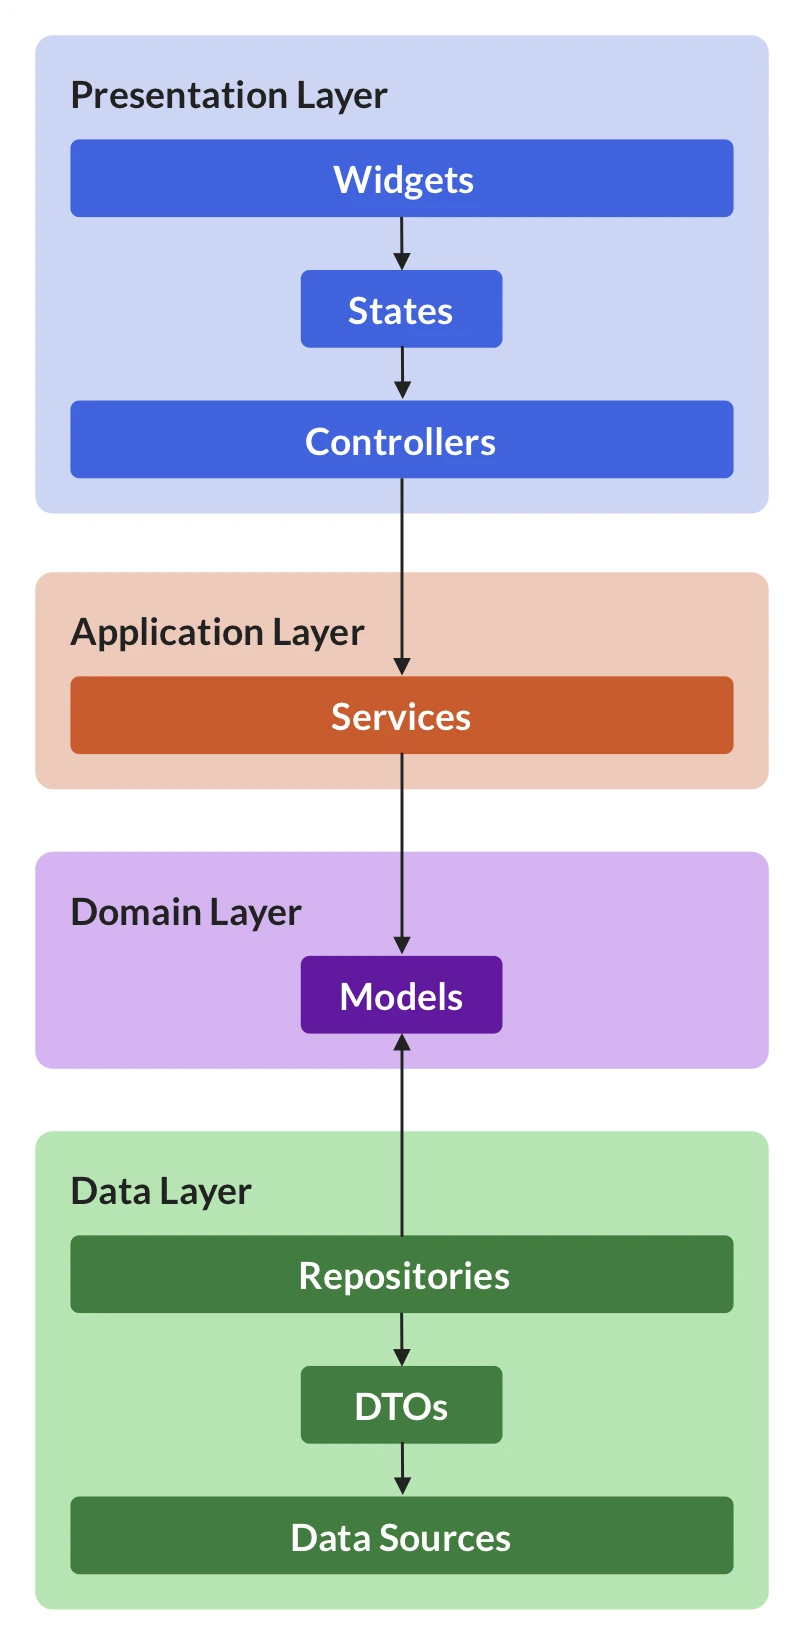
\includegraphics[height=10cm]{images/Flutter2.png}
    \caption{Cheyyan System Diagram depicting the connections between components.}
    \label{fig:cheyyan_system_diagram}
\end{figure}

\subsection{System Diagram}

Figure \ref{fig:cheyyan_system_diagram} illustrates the complex interconnections between all of the components in the Cheyyan System. This graphic acts as a point of reference for comprehending the interactions and information flow inside the system.

% Insert System Diagram


\section{Design Process Overview}
For Cheyyan, a system aimed at gamifying Time Management, the design process was pivotal, focusing on intuitiveness and user-friendliness.

\subsection{Wire Frame}
Iterative development utilising Figma, a design tool that enabled a visual depiction of the application's layout and functionality, was part of the wireframing process for Cheyyan. Students' informal input was used to create wireframes.

\begin{figure}
\centering
\begin{minipage}{.5\textwidth}
  \centering
  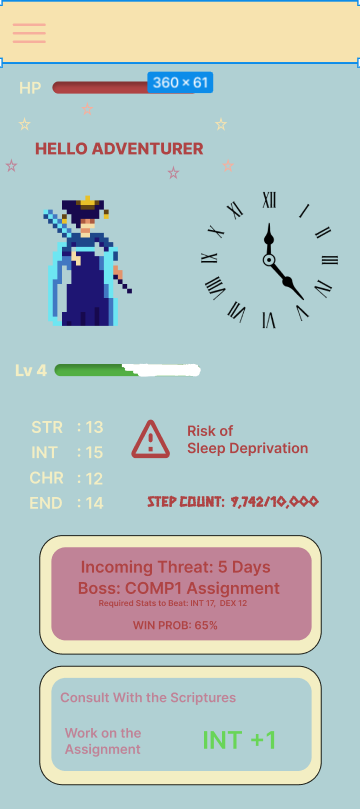
\includegraphics[width=.6\linewidth]{images/homepageWireFrame.png}
  \captionof{figure}{Homepage Wireframe}
  \label{fig:homepage_wireframe}
\end{minipage}%
\begin{minipage}{.5\textwidth}
  \centering
  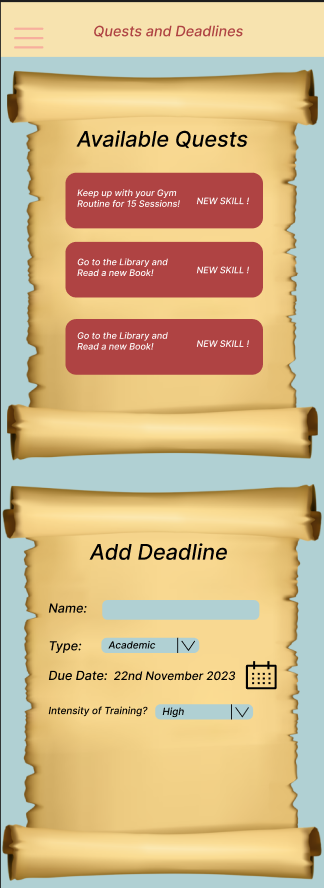
\includegraphics[width=.6\linewidth]{images/questsWireFrame.png}

  \caption{Quests Wireframe}
    \label{fig:Quests_wireframe}
\end{minipage}
\end{figure}

\begin{figure}[h]
    \centering
    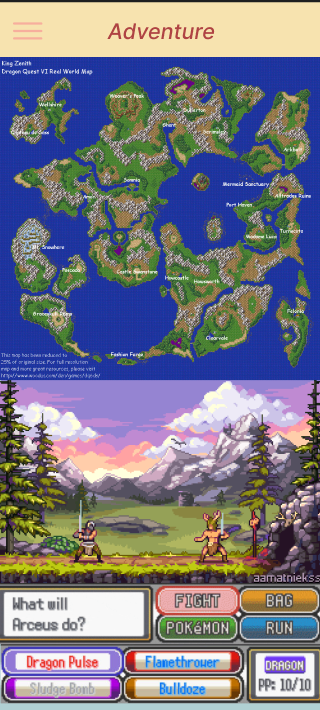
\includegraphics[height=10cm]{images/adventureWireframe.png}
    \caption{Proposed Adventure Screen Wireframe}
    \label{fig:adventure_wireframe}
\end{figure}



\subsection{
Exploring Design Evolution}
In Cheyyan, the evolution from wireframes to the finished product exposes fascinating subtleties that provide insights into the original conception and later changes. Interestingly, the wireframes display aspects of fantastical aesthetics that are different from the final iteration's simplified, practical style.

Imaginative elements that were discarded for the final product are seen in the wireframes. The 'Adventure Screen' (Fig \ref{fig:adventure_wireframe}), which was originally intended to be a gamified component of the application, serves as an example. This imagined minigame was intended to function as a kind of role-playing game, whereby players would be rewarded with abilities upon completing tasks, which would in turn influence interactions inside the application. This theoretical gamification component, meanwhile, was absent from the finished product.

In addition, the wireframes hint at a grandiose yet unfulfilled concept, a "Sleep Tracker" in the original Homepage, (Fig \ref{fig:homepage_wireframe}). The original idea was to incorporate a gamification element connected to health. If sleep is disturbed, users might face health consequences on the Adventure Screen. The idea was to establish a link between the virtual obstacles and physical health. However, this complex connection was dropped as the requirements for getting sleep data would have been something out of scope for such a small feature instead I opted in favour of a simpler strategy, which led to the addition of a "Reward Page." (Fig \ref{fig:Rewards}) This page increases the satisfaction that comes from finishing chores by acting as a positive reinforcement mechanism.

The design's transition from intricate fantasy details to a more sophisticated and practical style illustrates how the development process is iterative. It emphasises how the project may be adjusted to meet user demands and how features are prioritised to create a seamless and user-friendly experience. For example, you can see fantasy elements only in the naming conventions in the final product (Fig \ref{fig:Quests}) but in the Wireframe it is much more fantastical in design(Fig \ref{fig:Quests_wireframe}.  The academic exploration of these design decisions provides valuable insights into the dynamic interplay between conceptualization, user feedback, and the ultimate realization of a digital tool tailored for enhanced productivity and well-being.

Cheyyan's final version has undergone major improvements to improve user experience and highlight the app's essential features. The sign-up/login page (Fig \ref{fig:SignUp}), which provides users with the ease of Google authentication, is one noteworthy innovation. With this feature, users may access the app using their Google credentials, which not only makes the onboarding process easier but also increases security and trust.

Additionally, time management is given more of a focus across the Application, which is most noticeable on the updated calendar tab. Users may efficiently schedule and arrange their assignments, appointments, and events by using the calendar page as a primary hub. Users may easily browse, change, and manage their calendars with the help of user-friendly UI features and straightforward navigation, encouraging greater efficiency and productivity.

The calendar page also works well with other essential Cheyyan features like goal-setting and task management (Fig \ref{fig:Calendar}). Better coordination and planning of everyday activities are made possible by the ease with which tasks may be linked to certain dates and times. With the help of this integrated strategy, users may manage their time more effectively by prioritising their work, creating attainable objectives, and monitoring their advancement over time.

Moreover, the completed version of Cheyyan refocused on motivating and engaging users. Users are encouraged to stick to their time management objectives by use of gamified components and positive reinforcement systems. The implementation of daily challenges, incentives for task completion, and progress monitoring tools fosters a dynamic and engaging user experience that promotes habit-building and continued usage.



\begin{figure}
\centering
\begin{minipage}{.5\textwidth}
  \centering
  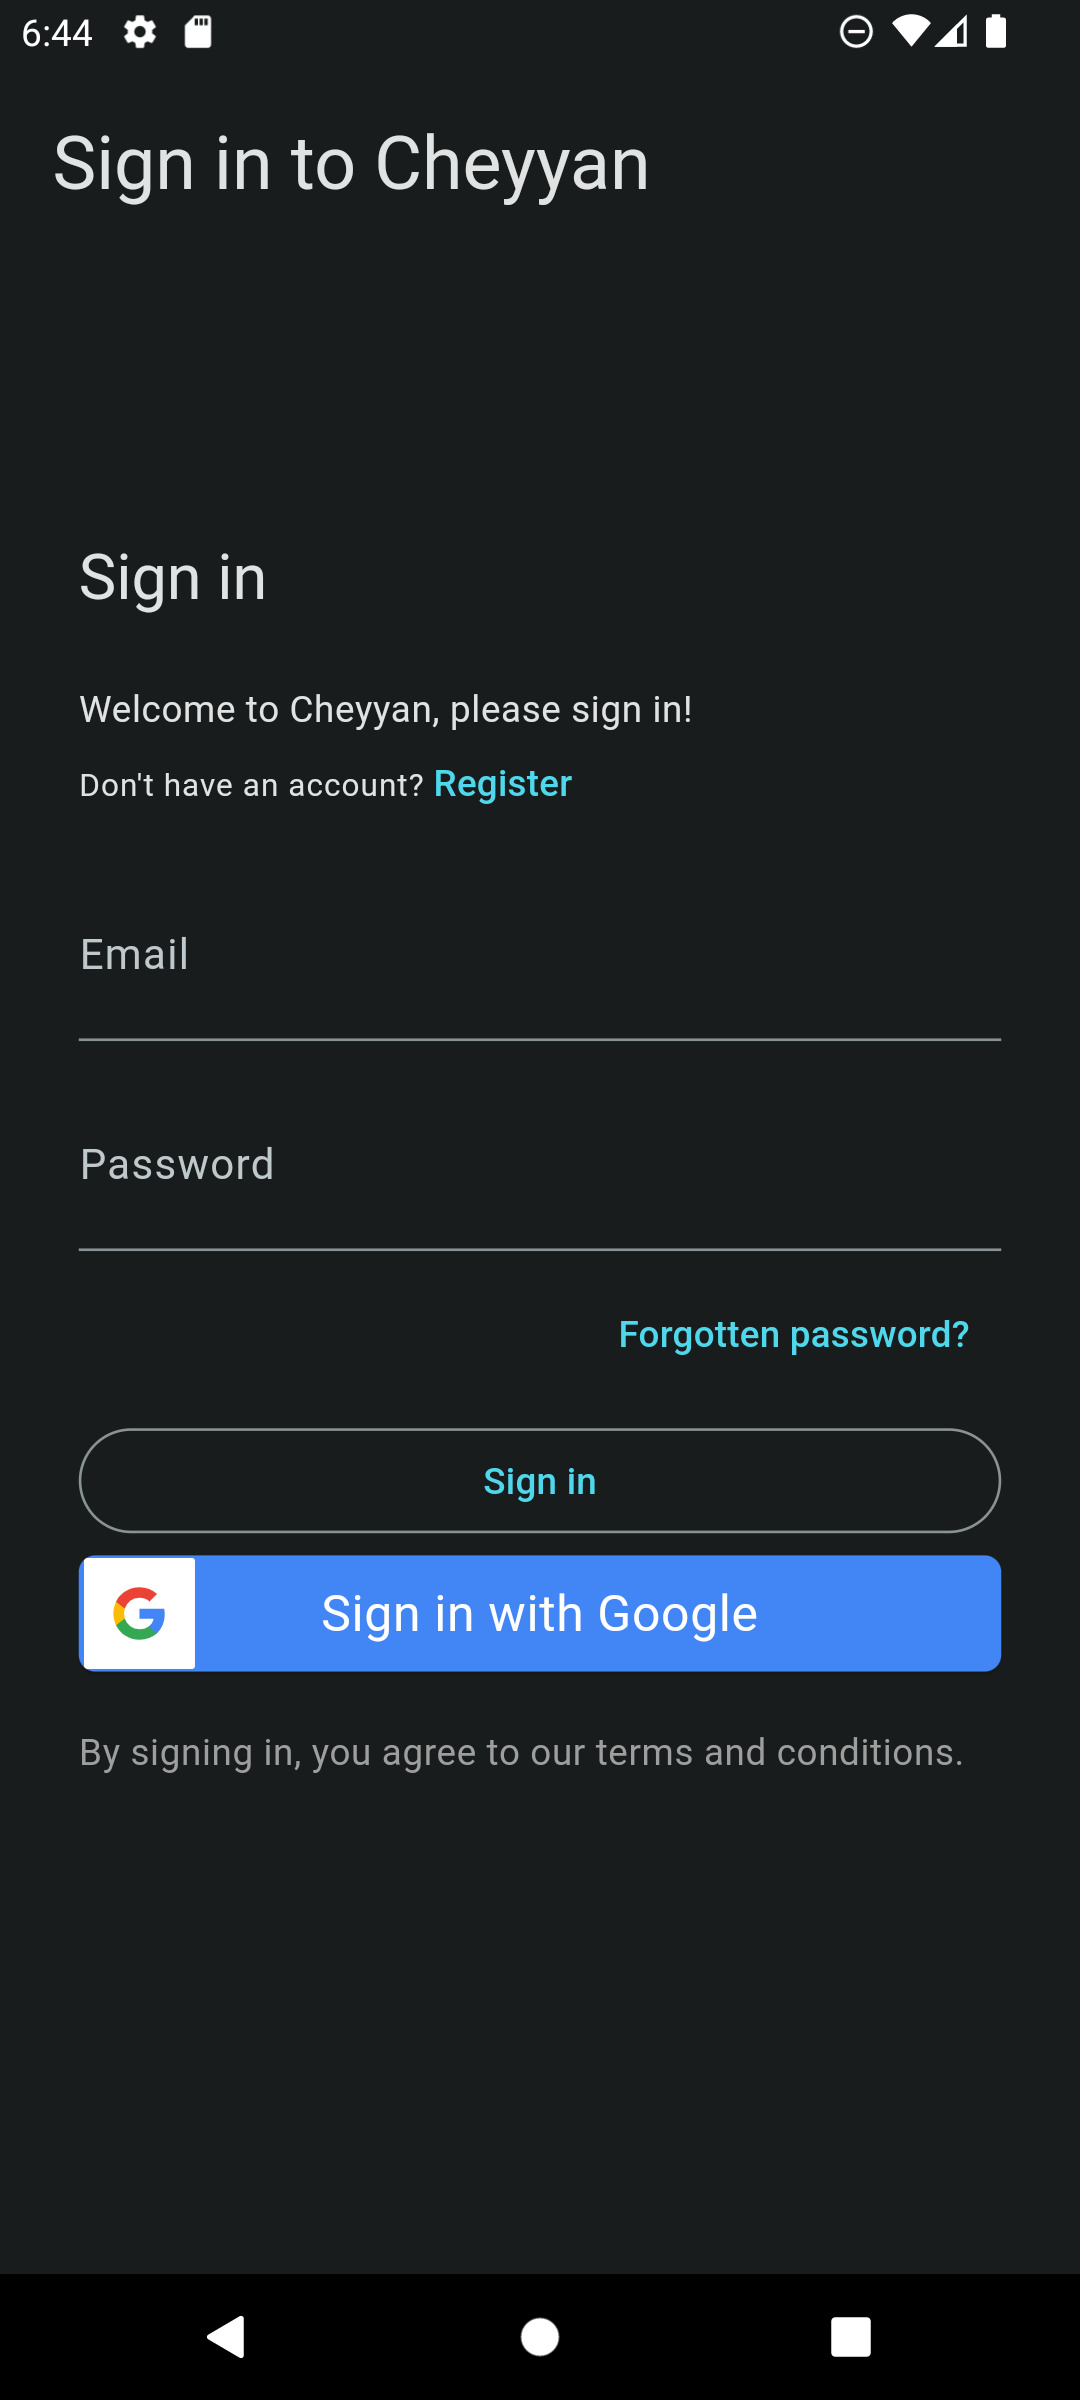
\includegraphics[width=.6\linewidth]{images/SignUp.png}
  \captionof{figure}{Sign Up and Log-In Page}
  \label{fig:SignUp}
\end{minipage}%
\begin{minipage}{.5\textwidth}
  \centering
  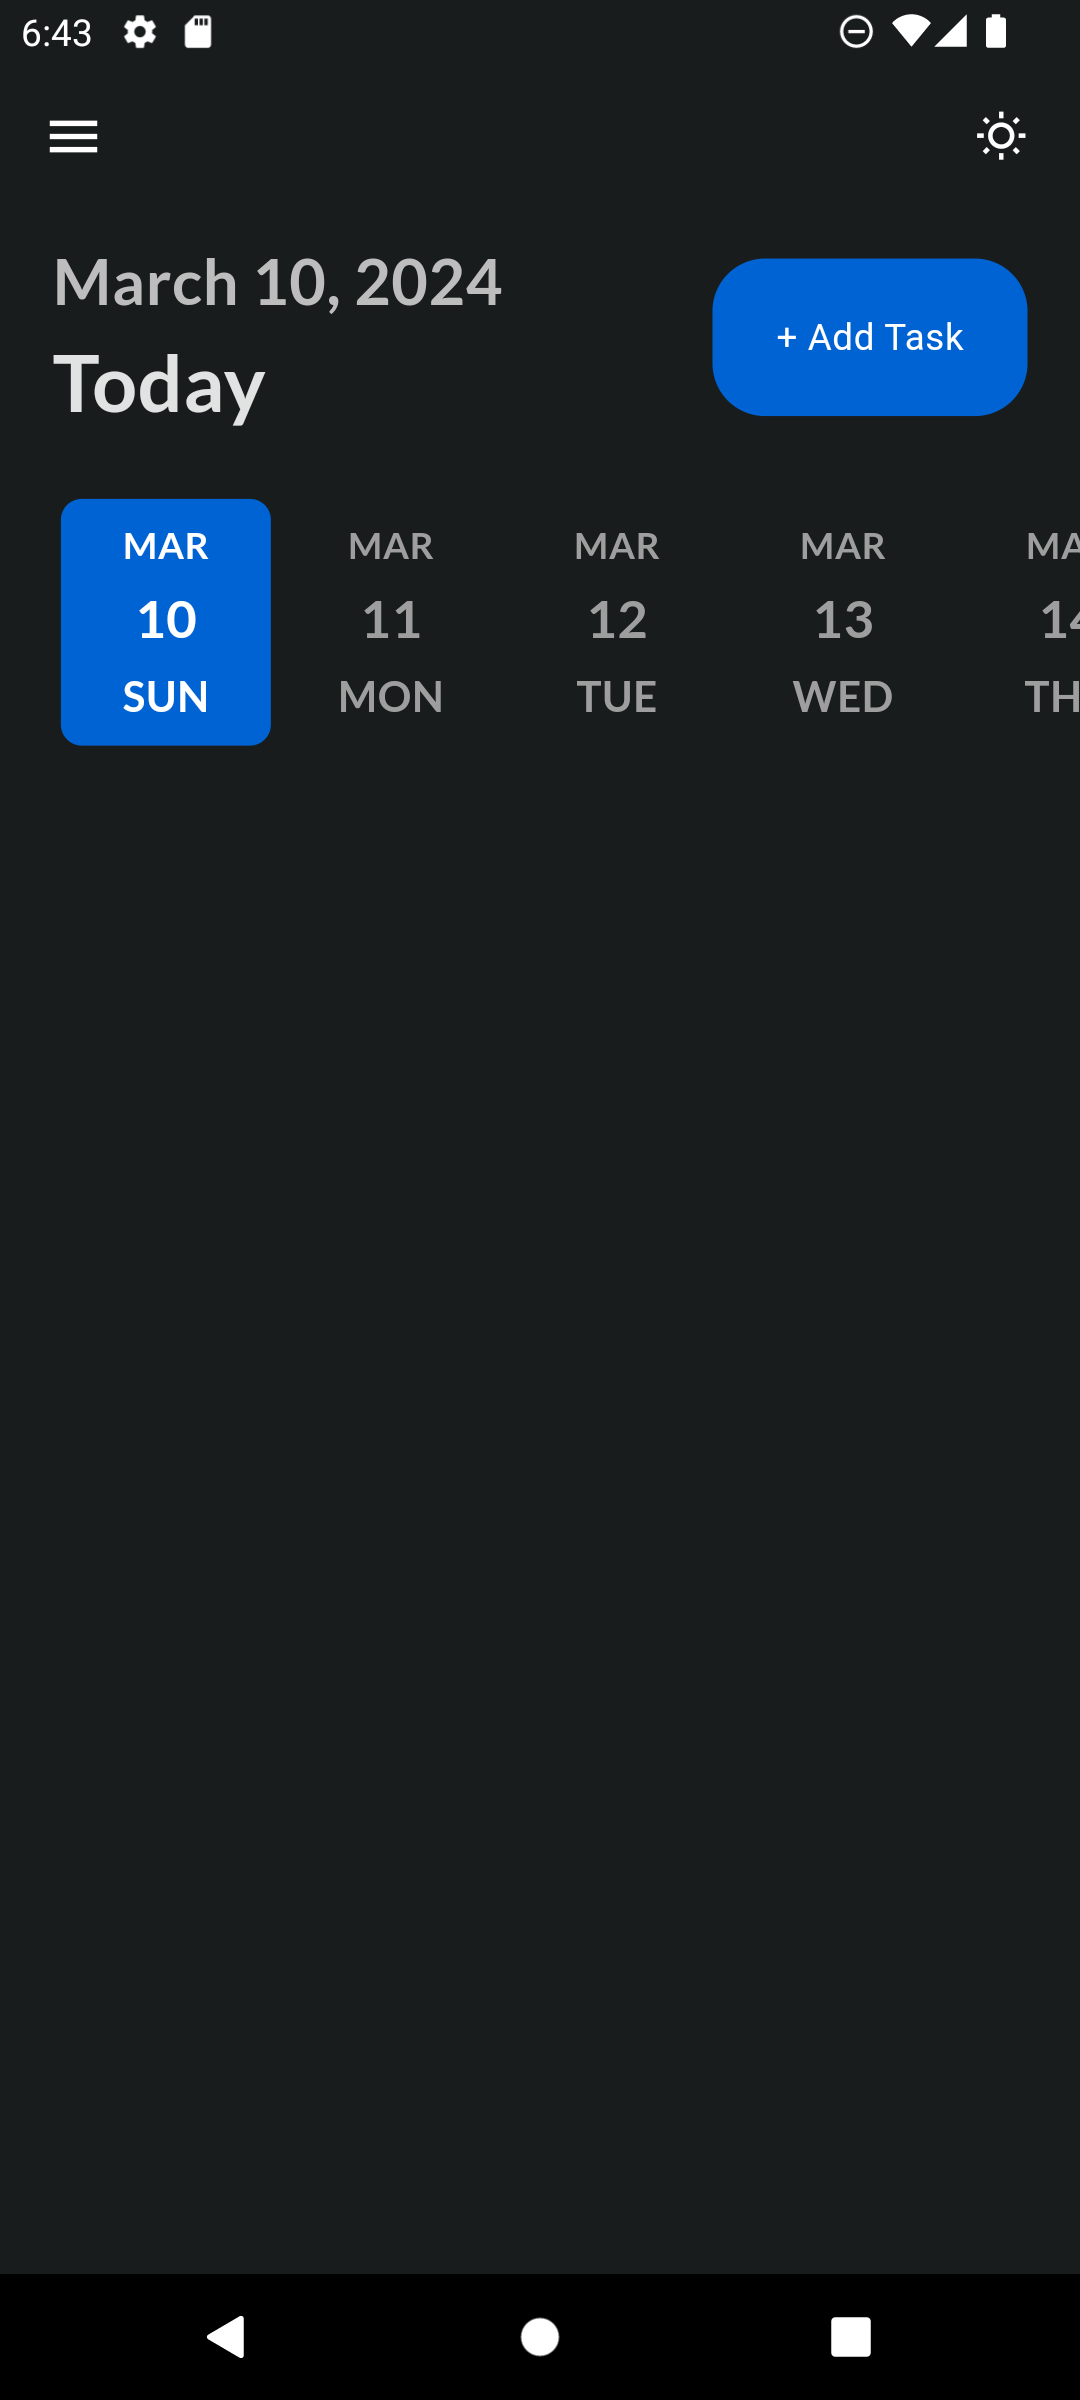
\includegraphics[width=.6\linewidth]{images/Calander.png}

  \caption{Calendar}
    \label{fig:Calendar}
\end{minipage}
\end{figure}

\begin{figure}
\centering
\begin{minipage}{.5\textwidth}
  \centering
  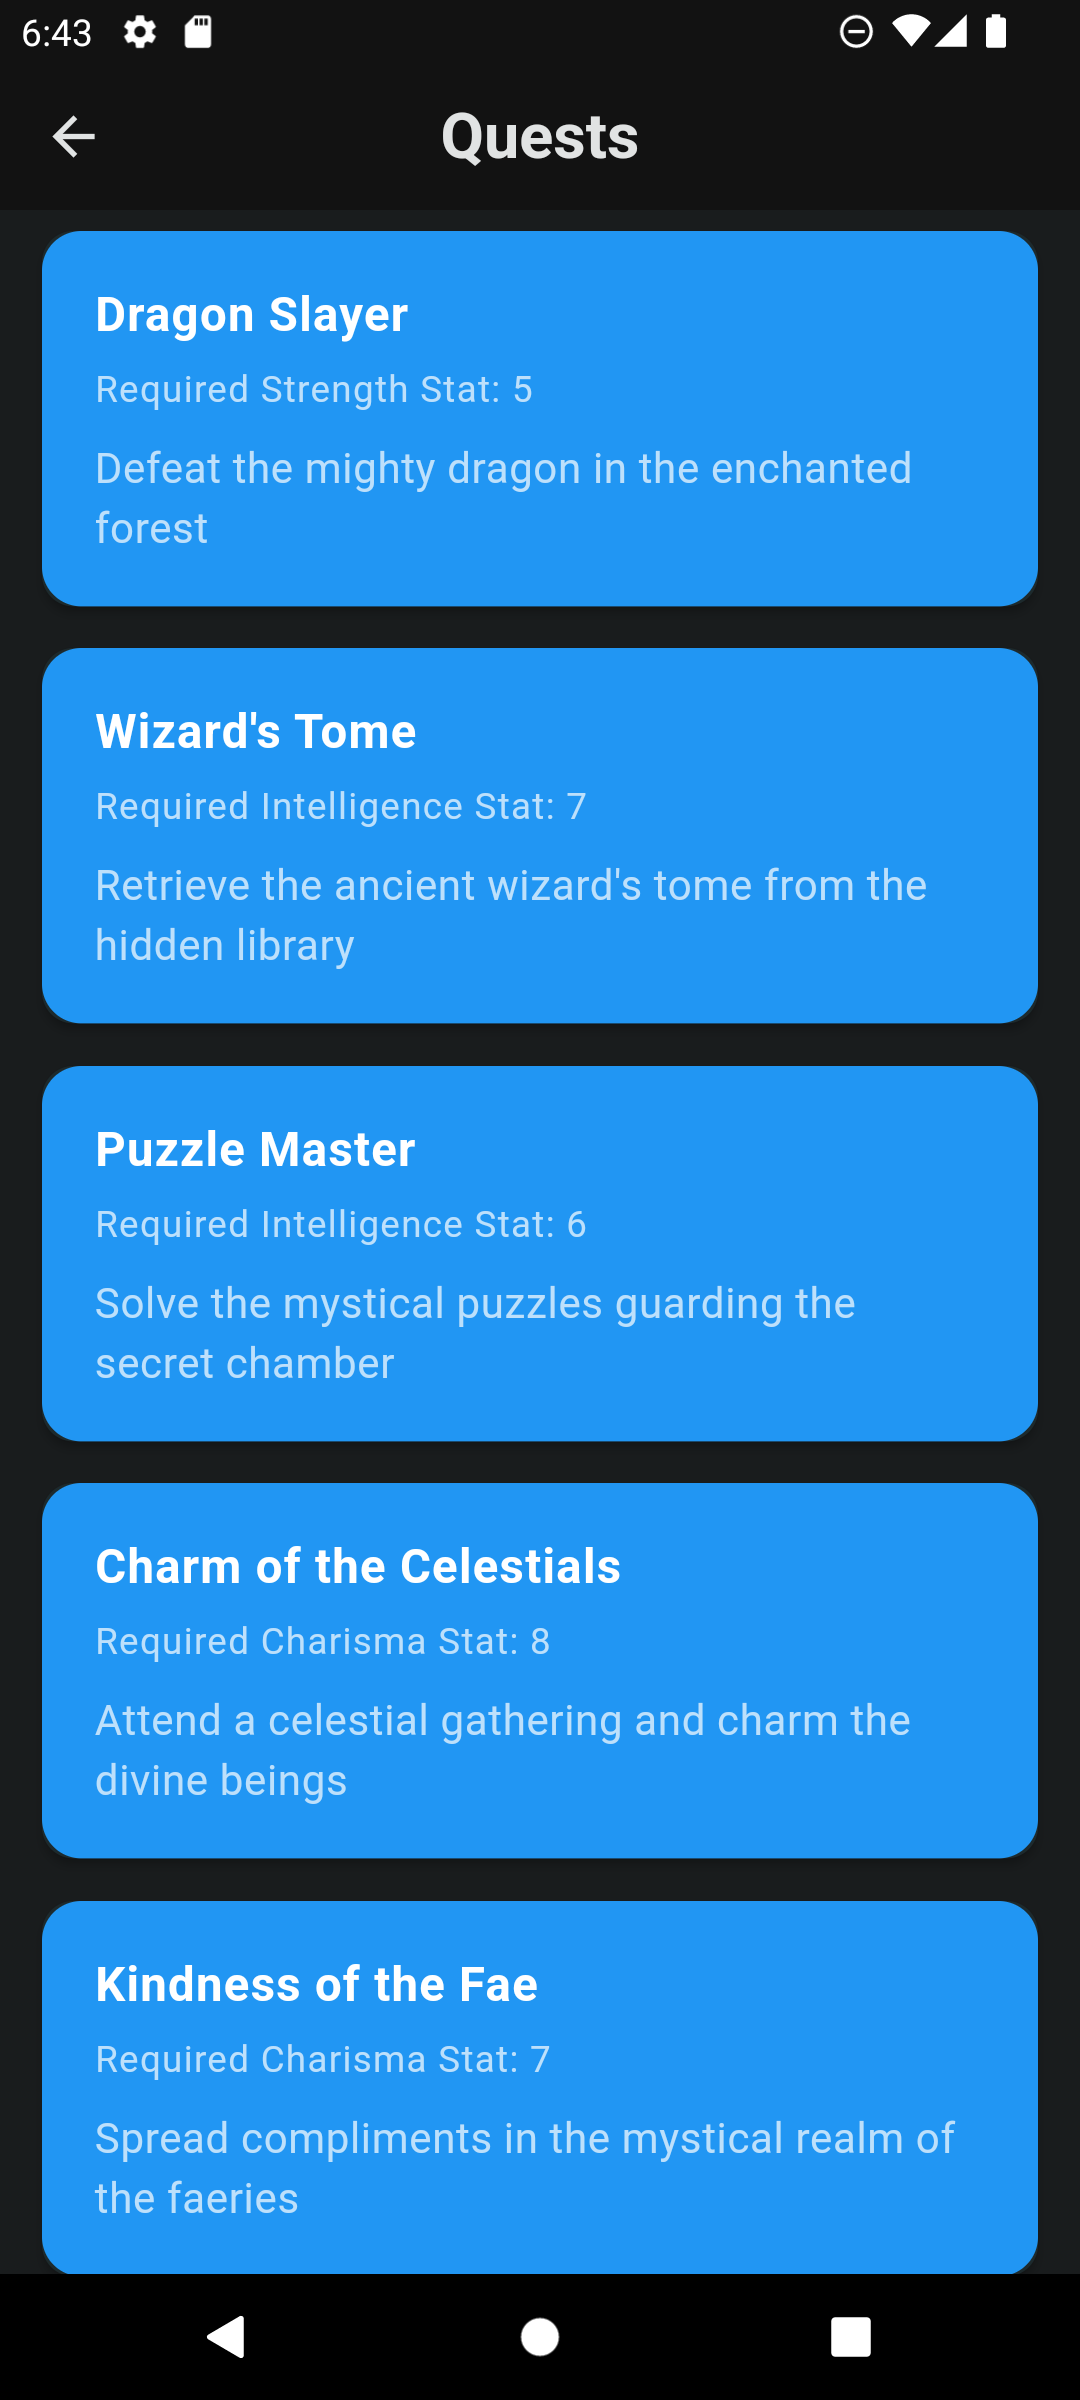
\includegraphics[width=.6\linewidth]{images/Quests.png}
  \captionof{figure}{Quests Page}
  \label{fig:Quests}
\end{minipage}%
\begin{minipage}{.5\textwidth}
  \centering
  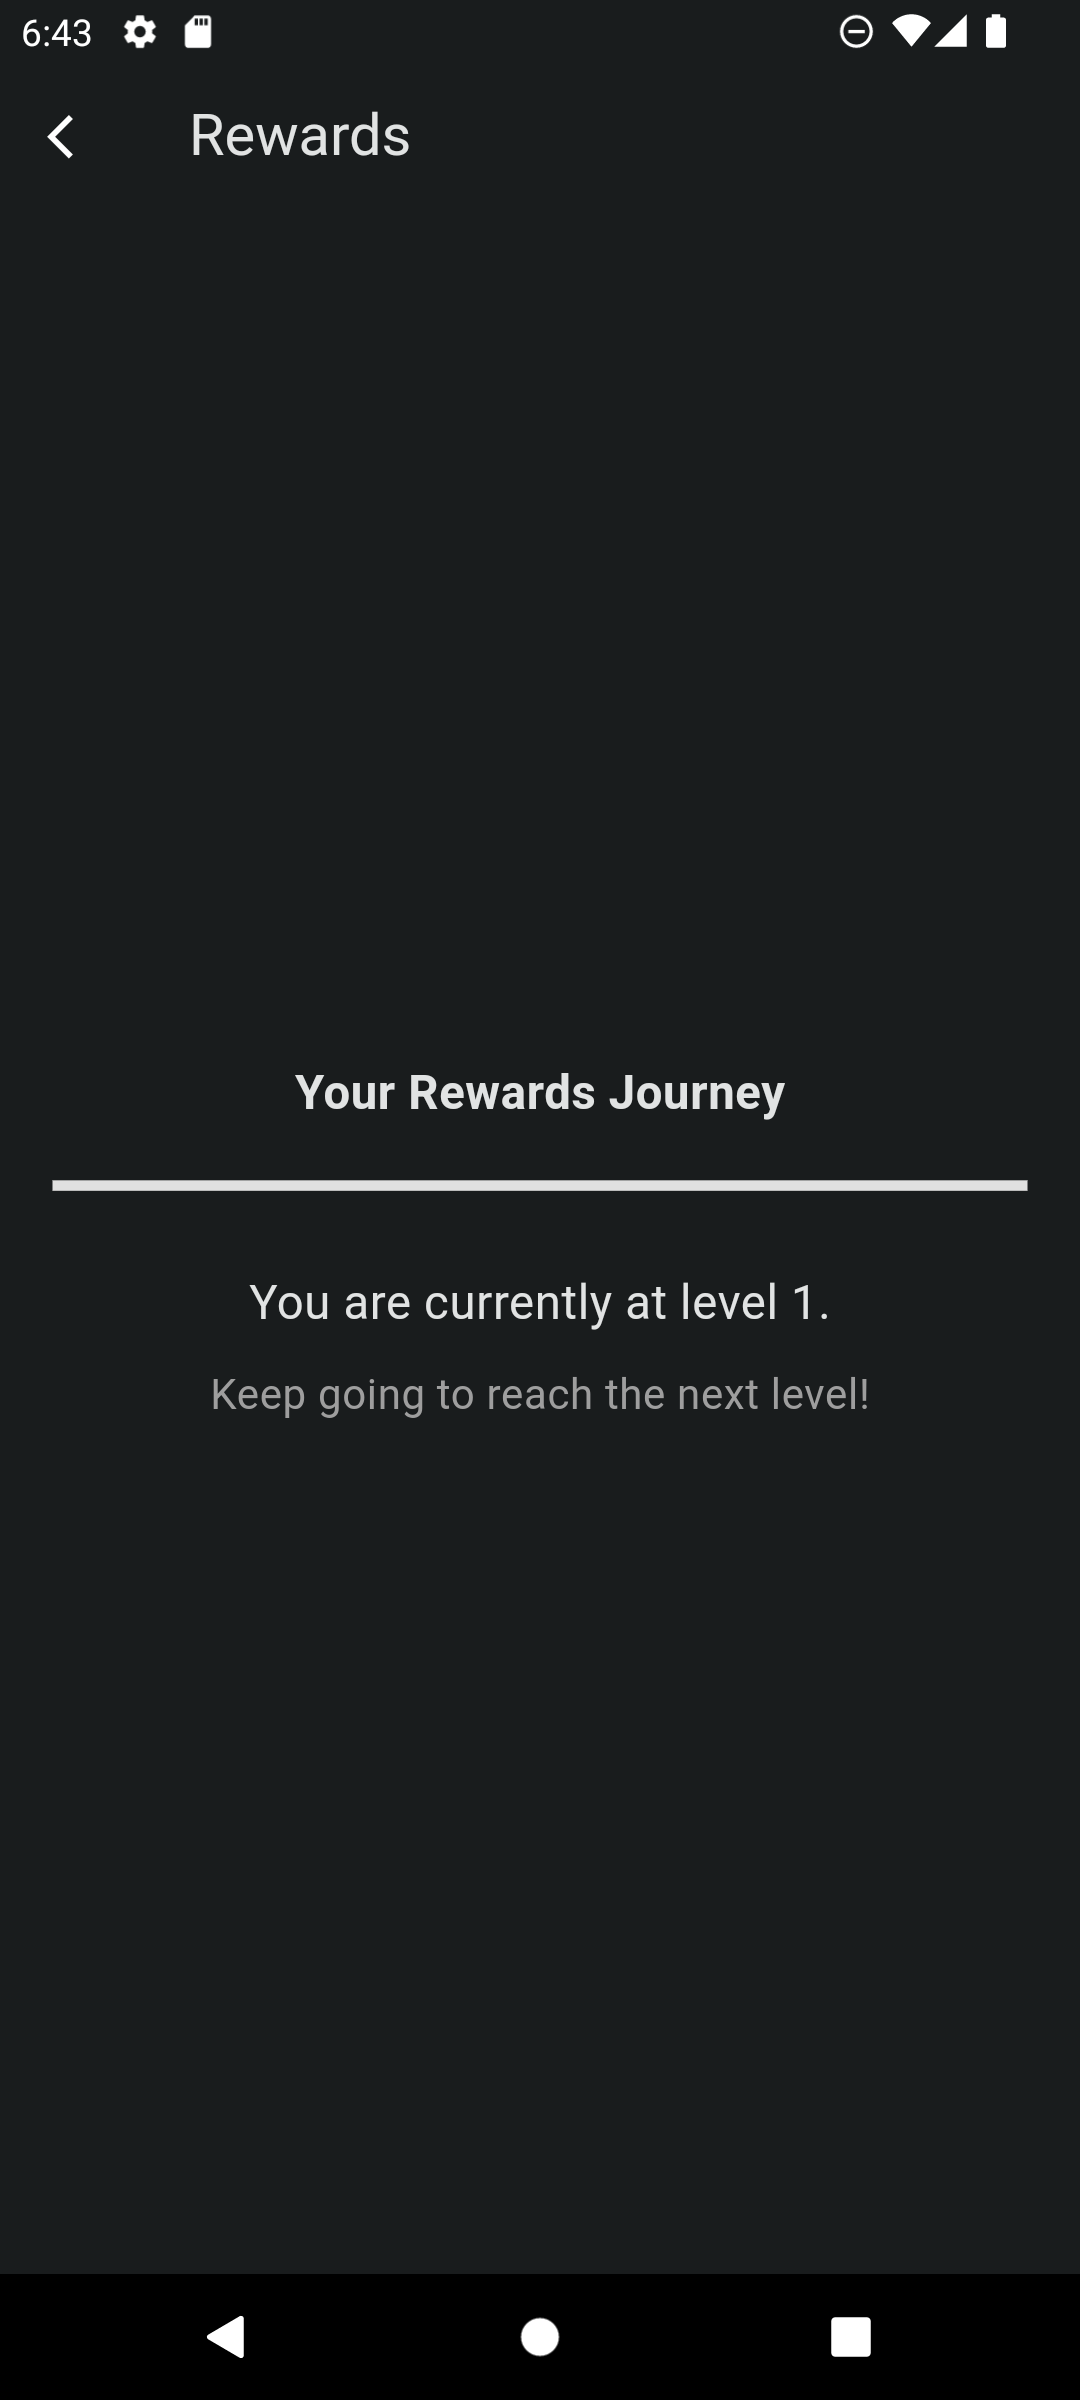
\includegraphics[width=.6\linewidth]{images/Rewards1.png}

  \caption{Rewards Page}
    \label{fig:Rewards}
\end{minipage}
\end{figure}

% \begin{figure}
% \centering
% \begin{minipage}{.5\textwidth}
%   \centering
%   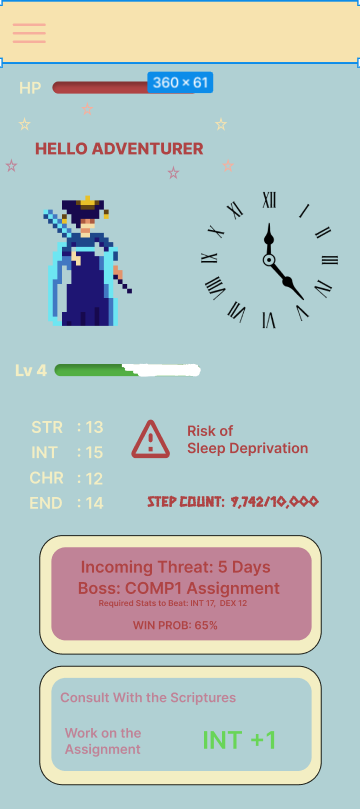
\includegraphics[width=.6\linewidth]{images/homepageWireFrame.png}
%   \captionof{figure}{Homepage Wireframe}
%   \label{fig:homepage_wireframe}
% \end{minipage}%
% \begin{minipage}{.5\textwidth}
%   \centering
%   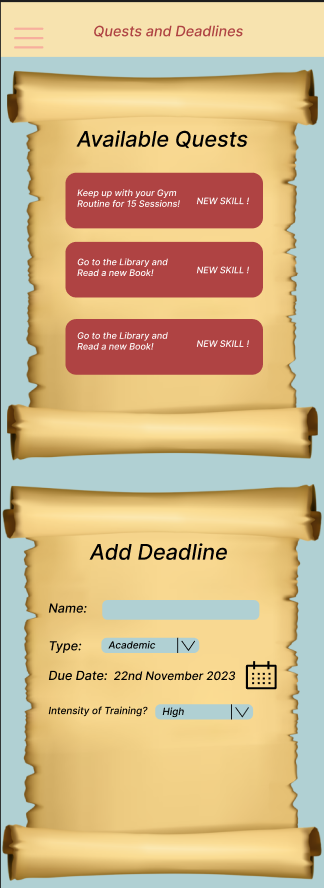
\includegraphics[width=.6\linewidth]{images/questsWireFrame.png}

%   \caption{Quests Wireframe}
%     \label{fig:Quests_wireframe}
% \end{minipage}
% \end{figure}






% \section{Design Ethics and Reasoning}
% A user-friendly interface is pivotal for Cheyyan to fulfill its functional requirements. The design encompasses features such as gamified elements, goal-setting, self-efficacy principles, positive reinforcement, intrinsic motivation, and accountability.


% \subsection{Gamified Elements}
% The inclusion of gamified elements introduces a fun and engaging experience for users. Cheyyan employs a comprehensive quest system where users embark on various challenges related to time management. Character development, tied to attributes such as strength (STR), intelligence (INT), charisma (CHR), and constitution (CON), adds a role-playing dimension to the user experience. Rewards earned through completing quests contribute to making time management a captivating endeavor, providing users with both tangible and intangible incentives to stay engaged.

% \subsection{Goal-Setting and Self-Efficacy}
% Cheyyan incorporates principles of goal-setting and self-efficacy, essential for effective time management. Users are encouraged to set SMART goals (Specific, Measurable, Achievable, Relevant, and Time-bound) through the system. The platform assists users in tracking their progress toward these goals, providing visual representations of achievements. This approach fosters a sense of accomplishment and self-efficacy, empowering users to take control of their time management practices.

% \subsection{Positive Reinforcement and Intrinsic Motivation}
% The focus on intrinsic motivation is central to Cheyyan's design philosophy. Positive reinforcement mechanisms are embedded in the system, rewarding users for completing quests and advancing in character development. By tapping into intrinsic motivation, Cheyyan aims to instill a lasting drive for behavioral change in time management practices. Users find satisfaction in the progress of their character, creating a positive feedback loop that promotes continuous engagement.

% \subsection{Accountability and Social Features}
% Cheyyan recognizes the importance of accountability in fostering positive behavioral change. The platform includes social features that enable users to connect with peers, parents, and teachers. This interconnectedness fosters a sense of accountability, as users can share their goals and progress with others. Parents and teachers, in particular, play a supportive role, providing encouragement and motivation. The social aspect enhances the overall user experience, transforming time management into a collaborative and rewarding journey.















% How is this problem to be approached, without reference to specific implementation details? 
% \section{Guidance}
% Design should cover the abstract design in such a way that someone else might be able to do what you did, but with a different language or library or tool.

%==================================================================================================================================
\chapter{Implementation}
Using different software engineering techniques, integrating backend services, and resolving
important implementation concerns and obstacles were all part of the Cheyyan implementation
stage. This synopsis sheds light on the development process while emphasising key elements of
Cheyyan’s architecture.

\section{Software Engineering Process}
\subsection{Version Control System}
Cheyyan used a methodical approach to software engineering, carefully selecting techniques that would improve development productivity. GitHub became the mainstay of version control, offering a cooperative code management environment. This protected against any data loss and allowed the development team to collaborate more easily. It also acted as a reliable backup system.

\subsection{Continuous Integration Tactics}
Although the original plan was to use Travis CI for continuous integration, several constraints forced a tactical change to manual inspections. Despite being unorthodox, this diversion was purposefully made to preserve an equilibrium between automation and the particular requirements of the undertaking. Manual checks gave the quality assurance procedure a personalised touch by guaranteeing a thorough examination of tests and linting services.

\begin{figure}[h]
    \centering
    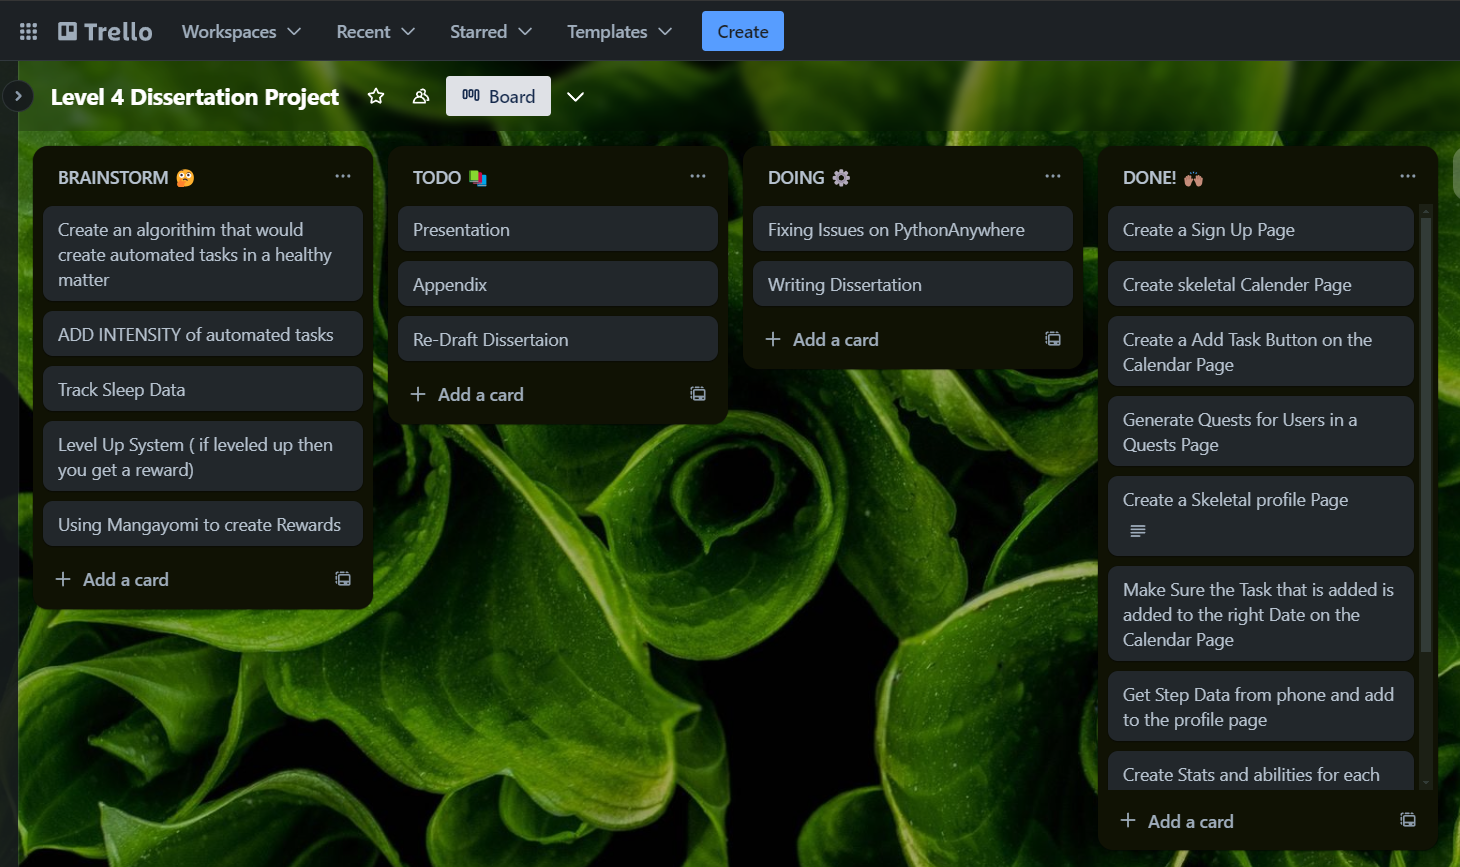
\includegraphics[height=10cm]{images/trello.png}
    \caption{Trello Board}
    \label{fig:Trello}
\end{figure}

\subsection{Agile Methodology Integration}
Cheyyan adopted an agile methodology concurrently, encouraging a flexible and iterative approach to development. This process made it possible to regularly review and modify plans to successfully meet changing requirements. The Trello board (Fig \ref{fig:Trello}), offers a visual depiction of activities at various levels, including "Brainstorm," "ToDo," "Doing" and "Done," was essential in the implementation of agile principles. This board made issue management easier and made time monitoring more efficient, which helped me assess how well tasks were being completed.

\subsection{Testing Practices in Agile Framework}
Cheyyan included unit tests and widget testing in its development process as part of an agile framework. The decision was driven by the need for extensive testing to guarantee the stability and dependability of the codebase. Although Travis CI and other continuous integration solutions may have made this process more efficient; the decision to opt for manual testing reflected a conscious effort to maintain a hands-on approach to quality assurance.

Cheyyan’s software engineering process was essentially a well-balanced combination of agile techniques, version control, and deliberate testing practice selections. The goal of this all-encompassing strategy was to establish a strong basis for the creation of an advanced time management system.

\section{Tools and Technologies in Cheyyan}
Considerations for the backend, frontend, databases, and potential integration with external tools define the technological foundation of Cheyyan.

\subsection{Backend}
The backend of Cheyyan leverages a robust framework, ensuring seamless integration and scalability to accommodate potential enhancements. The chosen backend framework for Cheyyan is SQLite, and it serves as the backbone of the platform’s functionality. SQLite is selected for its remarkable ability to handle complex operations, manage data efficiently, and provide a stable foundation for gamified features and user interactions. 

SQLite is a lightweight, embedded relational database management system that is widely recognised for its simplicity, reliability, and compatibility. Its serverless architecture and self-contained, file-based nature makes it an ideal choice for applications like Cheyyan, where a compact and efficient database solution is paramount. The use of SQLite aligns with Cheyyan’s goal to offer users a seamless and responsive experience while efficiently managing the data associated with quests, character development, and user interactions. 

The advantages of using SQLite extend to its ease of integration, low maintenance overhead, security and compatibility with various platforms. Its support for SQL queries facilitates the implementation of complex database operations, ensuring that Cheyyan can handle the diverse tasks related to time management and gamification. With SQLite as the backend framework, Cheyyan is well-positioned to provide a reliable and efficient platform for users to enhance their time management skills.


\section*{Firebase}
Robust user authentication was made possible in Cheyyan thanks in large part to Firebase, a feature-rich mobile and web application development platform provided by Google. Because of Firebase’s large feature set, scalability, and easy integration, this solution was chosen for user authentication.



\subsection*{Important Firebase Authentication Features:}

\begin{itemize}
  \item \textbf{Secure and Scalable:}Firebase Authentication utilises industry-accepted security protocols to guarantee the privacy and accuracy of user credentials. The platform’s easy scalability allows it to accommodate Cheyyan’s expanding user base without sacrificing security.

  \item \textbf{Email and Password Authentication:} 
 Users may easily and securely establish accounts with Firebase’s simple email and password authentication technique. For productivity software like Cheyyan, this technique is essential to maintaining the privacy of user data.

  \item \textbf{Social Media Integration:}Users may sign in with their current Google, Facebook, or other supported service accounts thanks to Firebase Authentication's seamless integration with major social networking platforms. This promotes wider user acceptance and improves user ease.

  \item \textbf{Multi-Factor Authentication (MFA):} Firebase facilitates multi-factor authentication (MFA) in order to improve security posture. Users of Cheyyan have the choice to activate MFA, which gives their accounts an extra degree of security.
\end{itemize}

\section*{Integration Rationale:}

\begin{itemize}
  \item \textbf{Ease of Implementation:} Firebase offers an intuitive Software Development Kit (SDK) that makes it very easy to include authentication functionality into the Cheyyan application. The development cycle was sped up by the simplicity of implementation.
  
  \item \textbf{Real-time Synchronization:} User authentication status is continuously updated across devices thanks to Firebase's real-time database synchronisation. Functionality like the application's collaborative functionality and real-time data streaming depend on this real-time synchronisation.

  \item \textbf{Scalability:} Cheyyan must take scalability into account in order to attain a large user base. Since Firebase is a cloud-based platform, it can scale easily to meet variations in user traffic without sacrificing functionality.

  \item \textbf{Community and Support:} Firebase has a sizable and vibrant developer community that guarantees continuous assistance, frequent upgrades, and an abundance of tools. This ecosystem contributes to the long-term sustainability and reliability of the authentication system.
\end{itemize}

In conclusion, security, simplicity of integration, scalability, and a feature-rich toolkit were the main factors in Cheyyan's decision to choose Firebase for user authentication. Cheyyan's use of Firebase Authentication not only guarantees a dependable and safe user authentication procedure but also benefits from a flexible platform that adapts to the changing requirements of a dynamic productivity application.



\subsection{Frontend}
A dynamic and responsive front end is crucial for empowering users to interact effortlessly with Cheyyan's gamified features. The frontend is developed using standard Flutter widgets, harnessing the inherent capability of Flutter to create engaging and user-friendly interfaces. This pragmatic choice enables Cheyyan to deliver a visually appealing and intuitive user experience, contributing to the platform's overall effectiveness in supporting users' time management goals.

\subsubsection{Performance}
The use of standard Flutter widgets contributes to Cheyyan's performance optimization. Flutter's framework ensures high rendering speeds by compiling the UI components into native ARM code, eliminating the need for a JavaScript bridge. This approach enhances Cheyyan's responsiveness, providing users with a smooth and seamless experience while navigating through gamified features and interactions.

\subsubsection{Accessibility}
Cheyyan prioritizes accessibility by adhering to Flutter's built-in accessibility features. Flutter widgets inherently support accessibility functionalities, ensuring that users with diverse needs can engage with the platform effectively. Features like screen reader compatibility and customizable text sizes enhance the overall accessibility of Cheyyan.

\subsubsection{Cross-browser Compatibility}
Given that Cheyyan is a mobile application built with Flutter, cross-browser compatibility is not applicable. Flutter primarily focuses on mobile platforms, and the rendering is optimized for iOS and Android. However, this design decision aligns with Cheyyan's mobile-centric approach, ensuring a consistent and optimized experience across supported devices.

\subsubsection{Single Point of Failure (SPoF)}
To mitigate the risk of a single point of failure, Cheyyan incorporates a robust backend architecture and employs redundancy strategies. The backend services are distributed across reliable server environments, reducing the likelihood of a SPoF. Additionally, Cheyyan implements error handling and monitoring mechanisms to detect and address potential issues promptly.

\subsubsection{Scalability}
Flutter's architecture facilitates scalability, allowing Cheyyan to accommodate an increasing user base seamlessly. As user demand grows, the backend infrastructure can be horizontally scaled, distributing the load efficiently. The use of Flutter widgets promotes consistency in UI components, easing the scaling process and ensuring a uniform user experience.

\subsubsection{Security}
Security is a paramount consideration for Cheyyan's design. The backend framework, SQLlite, is chosen for its robust security features, ensuring the safe management of complex operations and user data. Additionally, Cheyyan follows best practices for secure communication, data storage, and user authentication to safeguard user information.

\subsubsection{Data State Consistency}
Maintaining data consistency between the mobile and desktop versions of Cheyyan is achieved through a synchronized backend database. The use of SQLite ensures data integrity, and regular synchronization processes are implemented to update user data seamlessly across devices. This approach guarantees that users experience a coherent and up-to-date state of their progress and goals.

\subsubsection{Flutter: Pros and Cons}
Flutter offers several advantages, including a single codebase for iOS and Android, a rich set of pre-designed widgets, and hot-reload functionality for efficient development. However, potential challenges include a larger app size due to the inclusion of the Flutter engine, limited access to certain platform-specific features, and a learning curve for developers new to the framework. Despite these considerations, the decision to use Flutter aligns with Cheyyan's goal of providing a consistent and engaging user experience across multiple platforms.

\subsection{Integration with External Tools}
Cheyyan is thoughtfully crafted to seamlessly integrate with various external tools, showcasing its commitment to providing users with a comprehensive approach to time management. An exemplary instance of this integration involves leveraging PythonAnywhere to host a Python script interfacing with the Libgen API. This strategic decision enhances Cheyyan's functionality, allowing users to seamlessly import tasks and schedules directly into the platform.\\

\subsubsection{LibGen API}
The Library Genesis API, or LibGen API, is a technological entry point to the extensive collection of academic publications and works that Library Genesis hosts. Developers working on the Cheyyan application, for example, can programmatically get metadata and book and publisher details using the endpoints exposed by this API. The technical details include creating HTTP queries to certain endpoints that, in turn, return structured data. For easy integration into apps, this data usually contains information on book titles, authors, publishing years, and download URLs.

However, using the LibGen API changes the development environment by bringing in ethical issues. As Library Genesis distributes copyrighted content without explicit permission, there has been concern around the platform. Although the API is a neutral mechanism for data access, using it in apps poses ethical concerns about unintentionally aiding in the distribution of copyrighted information.

Cheyyan takes a responsible stance and doesn't give out copyrighted products as prizes in order to negotiate this morally tricky area. The application chooses to reward users with Open Domain literature instead. Books in the open domain are those whose copyright has expired or are by those who have voluntarily entered the public domain. This reduces the possibility of copyright infringement and conforms to moral principles that support the responsible use of intellectual property.

In addition to following legal requirements, the choice to stay away from copyrighted assets highlights Cheyyan's dedication to moral software development methods. Cheyyan finds a compromise between using the priceless resources made available by the LibGen API and respecting moral guidelines for content sharing by selecting Open Domain books as prizes. By taking this strategy, the application may continue to be a responsible member of the digital ecosystem, providing users with worthwhile incentives while adhering to copyright regulations. \\


\subsubsection{Flutter Packages}
The integration process involves the utilization of popular Flutter packages such as \\flutter\_local\_notifications, http, url\_launcher, and others. These Flutter packages play a crucial role in facilitating smooth communication between Cheyyan and the external Python script hosted on PythonAnywhere. Notably, this integration extends beyond conventional mobile application practices, incorporating server-side scripting to fetch reward download links from the Libgen API.

A key component of Cheyyan's development has been the integration of Firebase-related packages, such as Firebase Authentication and Firebase Realtime Database. Strong and secure user authentication techniques are provided by Firebase Authentication, a crucial component. Ensuring the confidentiality and integrity of user credentials is crucial in order to protect user data and comply with modern security requirements. On the other hand, smooth real-time synchronisation of user data across devices is made possible via the Firebase Realtime Database. Supporting capabilities like real-time data streaming and collaborative Cheyyan functions are made possible by this technology. These Firebase-related packages were chosen for integration because of their simplicity of use, ability to synchronise in real-time, and strong security features—all of which are essential for preserving a dependable and intuitive application.

Simultaneously, the addition of Flutter's Health package highlights Cheyyan's dedication to encouraging its consumers' overall well-being. Cheyyan goes beyond conventional work management by using health-related features, such as step counting via Google Fit and iOS Health APIs. The application gains a comprehensive dimension with the inclusion of health-related aspects, which recognise the connection between well-being and productivity. The Health package, which emphasises the value of incorporating wellness into technological solutions, is in line with current trends by encouraging consumers to maintain an active lifestyle and to be attentive to their health. This choice promotes Cheyyan as a holistic tool that addresses several aspects of users' lives in addition to broadening the application's usefulness.\\

\subsubsection{PythonAnywhere}
The adoption of PythonAnywhere as the hosting platform ensures the reliable and continuous availability of the Libgen API interfacing script. This approach aligns with Cheyyan's user-centric philosophy, providing users with enhanced flexibility and convenience in managing their time effectively. Users can seamlessly access and import tasks, schedules, and associated rewards, fostering a unified and synchronized experience across the Cheyyan platform.

The deliberate choice to host the Libgen API interface script on PythonAnywhere makes a substantial contribution to the consistent and dependable availability of this essential part of the Cheyyan ecosystem. This decision is based on the user-centric concept of Cheyyan, which seeks to provide consumers more freedom and ease in efficiently managing their time. Users may easily access and import tasks, schedules, and related incentives by utilising PythonAnywhere, which promotes a consistent and synchronised experience throughout the Cheyyan platform.

It is significant to note that obtaining a premium edition of PythonAnywhere was necessary for the execution of this solution. The free edition's restrictions on accessing the Libgen API and making it difficult to retrieve crucial data led to the need for the premium version. With its enhanced features, the paid version allowed for unrestricted communication with the Libgen API, circumventing the limitations of the free version. It's also important to note that the Libgen API works mainly with a list of carefully selected open-domain websites, which emphasises the necessity of a premium version to guarantee smooth data retrieval and Cheyyan platform integration. Cheyyan's dedication to providing consumers with a seamless and enhanced experience while using the Libgen API interface script is demonstrated by this strategic investment.

\subsection{Fitness API}
The smooth integration of the Google Fit and iOS Health App APIs allowed for the implementation of health and fitness tracking functions in Cheyyan. This calculated move was made with the intention of increasing user engagement by giving the application a complete, automatic step counter.

A safe and uniform method for allowing third-party apps restricted access to user data without disclosing private login credentials is made possible by OAuth 2.0. Users were requested to allow the Application to access their personal information in relation to Cheyyan's fitness monitoring. This authorization process adhered to industry best practices, prioritizing user privacy and data security.

Cheyyan was able to automatically measure users' daily steps thanks to the step counter feature obtained from these fitness APIs, which gave them important insights into their physical activity. This feature supports Cheyyan's overall well-being while also keeping up with the latest developments in the use of health data to provide individualised productivity tools.


Cheyyan emphasises that by using the Google Fit and iOS Health App APIs, Cheyyan underscores its commitment to user-centric design, fostering a more intuitive and integrated experience for individuals striving to manage their time effectively while prioritizing their health and well-being.

% % What did you do to implement this idea, and what technical achievements did you make?
% \section{Guidance}
% You can't talk about everything. Cover the high level first, then cover important, relevant or impressive details.



% \section{General points}

% These points apply to the whole dissertation, not just this chapter.


% \subsection{Figures}
% \emph{Always} refer to figures included, like Figure \ref{fig:relu}, in the body of the text. Include full, explanatory captions and make sure the figures look good on the page.
% You may include multiple figures in one float, as in Figure \ref{fig:synthetic}, using \texttt{subcaption}, which is enabled in the template.



% % Figures are important. Use them well.
% \begin{figure}
%     \centering
%     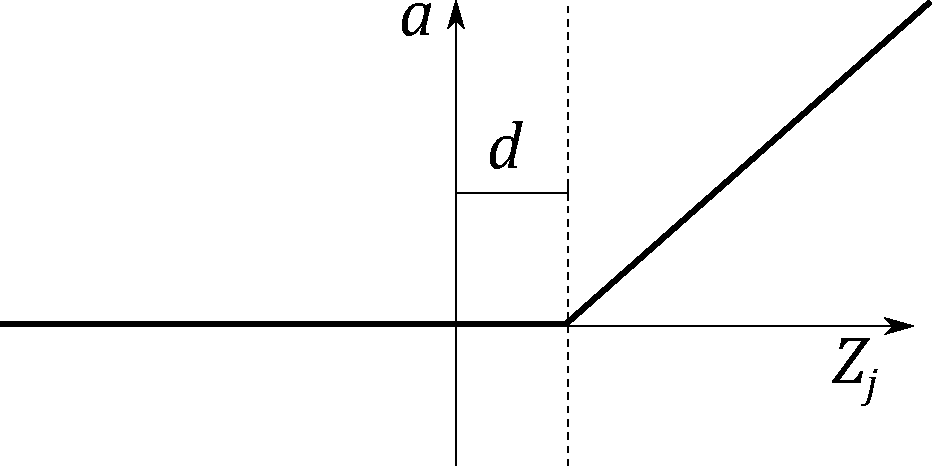
\includegraphics[width=0.5\linewidth]{images/relu.pdf}    

%     \caption{In figure captions, explain what the reader is looking at: ``A schematic of the rectifying linear unit, where $a$ is the output amplitude,
%     $d$ is a configurable dead-zone, and $Z_j$ is the input signal'', as well as why the reader is looking at this: 
%     ``It is notable that there is no activation \emph{at all} below 0, which explains our initial results.'' 
%     \textbf{Use vector image formats (.pdf) where possible}. Size figures appropriately, and do not make them over-large or too small to read.
%     }

%     % use the notation fig:name to cross reference a figure
%     \label{fig:relu} 
% \end{figure}


% \begin{figure}
%     \centering
%     \begin{subfigure}[b]{0.45\textwidth}
%         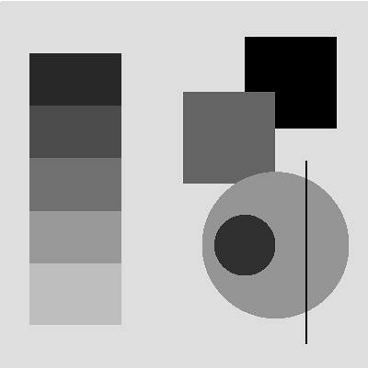
\includegraphics[width=\textwidth]{images/synthetic.png}
%         \caption{Synthetic image, black on white.}
%         \label{fig:syn1}
%     \end{subfigure}
%     ~ %add desired spacing between images, e. g. ~, \quad, \qquad, \hfill etc. 
%       %(or a blank line to force the subfigure onto a new line)
%     \begin{subfigure}[b]{0.45\textwidth}
%         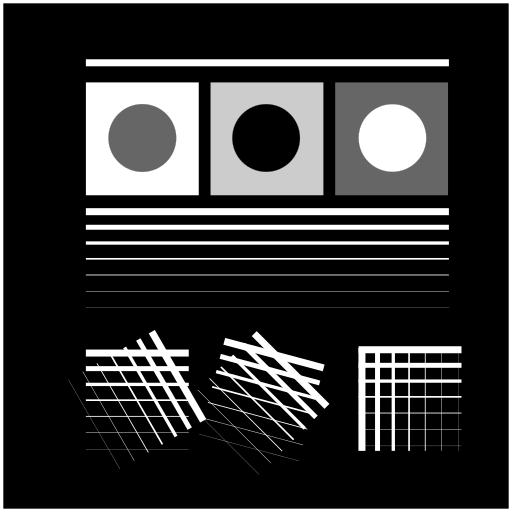
\includegraphics[width=\textwidth]{images/synthetic_2.png}
%         \caption{Synthetic image, white on black.}
%         \label{fig:syn2}
%     \end{subfigure}
%     ~ %add desired spacing between images, e. g. ~, \quad, \qquad, \hfill etc. 
%     %(or a blank line to force the subfigure onto a new line)    
%     \caption{Synthetic test images for edge detection algorithms. \subref{fig:syn1} shows various gray levels that require an adaptive algorithm. \subref{fig:syn2}
%     shows more challenging edge detection tests that have crossing lines. Fusing these into full segments typically requires algorithms like the Hough transform.
%     This is an example of using subfigures, with \texttt{subref}s in the caption.
%     }\label{fig:synthetic}
% \end{figure}

% \clearpage

% \subsection{Equations}

% Equations should be typeset correctly and precisely. Make sure you get parenthesis sizing correct, and punctuate equations correctly 
% (the comma is important and goes \textit{inside} the equation block). Explain any symbols used clearly if not defined earlier. 

% For example, we might define:
% \begin{equation}
%     \hat{f}(\xi) = \frac{1}{2}\left[ \int_{-\infty}^{\infty} f(x) e^{2\pi i x \xi} \right],
% \end{equation}    
% where $\hat{f}(\xi)$ is the Fourier transform of the time domain signal $f(x)$.

% \subsection{Algorithms}
% Algorithms can be set using \texttt{algorithm2e}, as in Algorithm \ref{alg:metropolis}.

% % NOTE: line ends are denoted by \; in algorithm2e
% \begin{algorithm}
%     \DontPrintSemicolon
%     \KwData{$f_X(x)$, a probability density function returing the density at $x$.\; $\sigma$ a standard deviation specifying the spread of the proposal distribution.\;
%     $x_0$, an initial starting condition.}
%     \KwResult{$s=[x_1, x_2, \dots, x_n]$, $n$ samples approximately drawn from a distribution with PDF $f_X(x)$.}
%     \Begin{
%         $s \longleftarrow []$\;
%         $p \longleftarrow f_X(x)$\;
%         $i \longleftarrow 0$\;
%         \While{$i < n$}
%         {
%             $x^\prime \longleftarrow \mathcal{N}(x, \sigma^2)$\;
%             $p^\prime \longleftarrow f_X(x^\prime)$\;
%             $a \longleftarrow \frac{p^\prime}{p}$\;
%             $r \longleftarrow U(0,1)$\;
%             \If{$r<a$}
%             {
%                 $x \longleftarrow x^\prime$\;
%                 $p \longleftarrow f_X(x)$\;
%                 $i \longleftarrow i+1$\;
%                 append $x$ to $s$\;
%             }
%         }
%     }
    
% \caption{The Metropolis-Hastings MCMC algorithm for drawing samples from arbitrary probability distributions, 
% specialised for normal proposal distributions $q(x^\prime|x) = \mathcal{N}(x, \sigma^2)$. The symmetry of the normal distribution means the acceptance rule takes the simplified form.}\label{alg:metropolis}
% \end{algorithm}

% \subsection{Tables}

% If you need to include tables, like Table \ref{tab:operators}, use a tool like https://www.tablesgenerator.com/ to generate the table as it is
% extremely tedious otherwise. 

% \begin{table}[]
%     \caption{The standard table of operators in Python, along with their functional equivalents from the \texttt{operator} package. Note that table
%     captions go above the table, not below. Do not add additional rules/lines to tables. }\label{tab:operators}
%     %\tt 
%     \rowcolors{2}{}{gray!3}
%     \begin{tabular}{@{}lll@{}}
%     %\toprule
%     \textbf{Operation}    & \textbf{Syntax}                & \textbf{Function}                            \\ %\midrule % optional rule for header
%     Addition              & \texttt{a + b}                          & \texttt{add(a, b)}                                    \\
%     Concatenation         & \texttt{seq1 + seq2}                    & \texttt{concat(seq1, seq2)}                           \\
%     Containment Test      & \texttt{obj in seq}                     & \texttt{contains(seq, obj)}                           \\
%     Division              & \texttt{a / b}                          & \texttt{div(a, b) }  \\
%     Division              & \texttt{a / b}                          & \texttt{truediv(a, b) } \\
%     Division              & \texttt{a // b}                         & \texttt{floordiv(a, b)}                               \\
%     Bitwise And           & \texttt{a \& b}                         & \texttt{and\_(a, b)}                                  \\
%     Bitwise Exclusive Or  & \texttt{a \textasciicircum b}           & \texttt{xor(a, b)}                                    \\
%     Bitwise Inversion     & \texttt{$\sim$a}                        & \texttt{invert(a)}                                    \\
%     Bitwise Or            & \texttt{a | b}                          & \texttt{or\_(a, b)}                                   \\
%     Exponentiation        & \texttt{a ** b}                         & \texttt{pow(a, b)}                                    \\
%     Identity              & \texttt{a is b}                         & \texttt{is\_(a, b)}                                   \\
%     Identity              & \texttt{a is not b}                     & \texttt{is\_not(a, b)}                                \\
%     Indexed Assignment    & \texttt{obj{[}k{]} = v}                 & \texttt{setitem(obj, k, v)}                           \\
%     Indexed Deletion      & \texttt{del obj{[}k{]}}                 & \texttt{delitem(obj, k)}                              \\
%     Indexing              & \texttt{obj{[}k{]}}                     & \texttt{getitem(obj, k)}                              \\
%     Left Shift            & \texttt{a \textless{}\textless b}       & \texttt{lshift(a, b)}                                 \\
%     Modulo                & \texttt{a \% b}                         & \texttt{mod(a, b)}                                    \\
%     Multiplication        & \texttt{a * b}                          & \texttt{mul(a, b)}                                    \\
%     Negation (Arithmetic) & \texttt{- a}                            & \texttt{neg(a)}                                       \\
%     Negation (Logical)    & \texttt{not a}                          & \texttt{not\_(a)}                                     \\
%     Positive              & \texttt{+ a}                            & \texttt{pos(a)}                                       \\
%     Right Shift           & \texttt{a \textgreater{}\textgreater b} & \texttt{rshift(a, b)}                                 \\
%     Sequence Repetition   & \texttt{seq * i}                        & \texttt{repeat(seq, i)}                               \\
%     Slice Assignment      & \texttt{seq{[}i:j{]} = values}          & \texttt{setitem(seq, slice(i, j), values)}            \\
%     Slice Deletion        & \texttt{del seq{[}i:j{]}}               & \texttt{delitem(seq, slice(i, j))}                    \\
%     Slicing               & \texttt{seq{[}i:j{]}}                   & \texttt{getitem(seq, slice(i, j))}                    \\
%     String Formatting     & \texttt{s \% obj}                       & \texttt{mod(s, obj)}                                  \\
%     Subtraction           & \texttt{a - b}                          & \texttt{sub(a, b)}                                    \\
%     Truth Test            & \texttt{obj}                            & \texttt{truth(obj)}                                   \\
%     Ordering              & \texttt{a \textless b}                  & \texttt{lt(a, b)}                                     \\
%     Ordering              & \texttt{a \textless{}= b}               & \texttt{le(a, b)}                                     \\
%     % \bottomrule
%     \end{tabular}
%     \end{table}
% \subsection{Code}

% Avoid putting large blocks of code in the report (more than a page in one block, for example). Use syntax highlighting if possible, as in Listing \ref{lst:callahan}.

% \begin{lstlisting}[language=python, float, caption={The algorithm for packing the $3\times 3$ outer-totalistic binary CA successor rule into a 
%     $16\times 16\times 16\times 16$ 4 bit lookup table, running an equivalent, notionally 16-state $2\times 2$ CA.}, label=lst:callahan]
%     def create_callahan_table(rule="b3s23"):
%         """Generate the lookup table for the cells."""        
%         s_table = np.zeros((16, 16, 16, 16), dtype=np.uint8)
%         birth, survive = parse_rule(rule)

%         # generate all 16 bit strings
%         for iv in range(65536):
%             bv = [(iv >> z) & 1 for z in range(16)]
%             a, b, c, d, e, f, g, h, i, j, k, l, m, n, o, p = bv

%             # compute next state of the inner 2x2
%             nw = apply_rule(f, a, b, c, e, g, i, j, k)
%             ne = apply_rule(g, b, c, d, f, h, j, k, l)
%             sw = apply_rule(j, e, f, g, i, k, m, n, o)
%             se = apply_rule(k, f, g, h, j, l, n, o, p)

%             # compute the index of this 4x4
%             nw_code = a | (b << 1) | (e << 2) | (f << 3)
%             ne_code = c | (d << 1) | (g << 2) | (h << 3)
%             sw_code = i | (j << 1) | (m << 2) | (n << 3)
%             se_code = k | (l << 1) | (o << 2) | (p << 3)

%             # compute the state for the 2x2
%             next_code = nw | (ne << 1) | (sw << 2) | (se << 3)

%             # get the 4x4 index, and write into the table
%             s_table[nw_code, ne_code, sw_code, se_code] = next_code

%         return s_table

% \end{lstlisting}

%==================================================================================================================================
\chapter{Evaluation} 
This chapter contains our review of Cheyyan, with an emphasis on how well it works to help students manage stress and maintain a work-life balance. The goal of the assessment method was to ascertain how much the deployed features help users manage their stress and tasks. The aim is to critically evaluate Cheyyan's effectiveness in enhancing time management skills through gamification elements.

\section{Evaluation Methodology}

Our evaluation process sought to evaluate users' experiences with the time management software Cheyyan—which has gamification components—in its entirety. To do this, we created a structured survey that included a wide range of features related to user interaction and the operation of the app. The survey was carefully designed to gather information on several important topics, such as task management, quest fulfilment, app performance, incentive system, and overall satisfaction and was supervised by me.

The survey was navigated by the participants and had discrete parts that corresponded to various facets of their interactions with Cheyyan. A comprehensive picture of users' perspectives and experiences was made possible by the careful crafting of each component to elicit particular comments. We intended to gather a wide range of insights by designing the survey in this way, making sure no crucial component of the app's operation was overlooked.

The sections of the survey were as follows:

\begin{enumerate}
    \item \textbf{App Navigation}: The purpose of this section was to evaluate how simple it was to navigate Cheyyan's UI. Participants were asked to rate how easily accessible the main functions were and how intuitive the app's interface was.
    
    \item \textbf{Task Management}: Participants were asked to discuss their Cheyyan task addition and management experiences. The purpose of this part was to evaluate how well the software helped users prioritise their tasks and organise their responsibilities.
    
    \item \textbf{Quest Completion}: Here, users were asked to provide their opinions about how they interacted with Cheyyan's quest completion system. This involved rating the quest interface's ease of use, the quest instructions' clarity, and overall satisfaction with the quest-based work management method.
    
    \item \textbf{Reward System}: Questions on the participants' experiences with Cheyyan's reward system, which provides incentives for users to finish activities, were asked. We asked for feedback on the incentives' applicability, how simple it was to redeem them, and how satisfied people were overall with the reward system.
    
    \item \textbf{App Performance}: The technical performance of Cheyyan, including any latency, crashes, or other bugs, was assessed in this area. When using the app, participants were asked to report any problems they had with performance.
    
    \item \textbf{Total Contentment}: In the last portion, participants were asked how satisfied they were overall with Cheyyan. This included their overall opinions on the app, whether they planned to use it going forward, and if they would suggest it to others.
\end{enumerate}

The survey's results were gathered anonymously to promote open communication. By remaining anonymous, members would feel free to voice their thoughts without worrying about criticism or negative consequences. To guarantee that the feedback received was authentic and accurately represented consumers' actual experiences with Cheyyan, we placed a high priority on privacy.

\section{Data Collection and Participant Interaction}
Given the limitations and research aims of the study, we decided to employ a survey to gather data for our evaluation of Cheyyan. Numerous variables contributed to this choice.

\begin{enumerate}
  
  \item \textbf{Scalability}: A survey makes it possible to effectively gather information from lots of people at once. Because Cheyyan may have a large user base, this scalability was crucial to obtaining a wide range of perspectives and experiences in a fair amount of time.
  
  \item \textbf{Standardisation}: Surveys make it possible to standardise questionnaire forms and data-gathering techniques. We established consistency in the sorts of data collected by giving participants a structured series of questions, which made it simpler to compare and analyse replies from various people.
  
\item \textbf{Anonymity}: Participants may voice their thoughts freely in surveys without worrying about prejudice or judgment because of the degree of anonymity they provide. Sincerity and openness in comments are encouraged by this anonymity, which results in more trustworthy and sincere feedback on the features and operation of the application.
  
  \item \textbf{Ease of Administration}: Compared to other data-gathering techniques like interviews or observational studies, surveys are comparatively easy to run, needing little in the way of resources and administrative work. Because of its simplicity, the data-collecting procedure was streamlined and a wider pool of possible participants could be reached.
  
  \item \textbf{Accessibility}: Since surveys can be sent and completed remotely, a broad spectrum of people can participate, regardless of time or location restrictions. This accessibility guaranteed participant recruitment inclusiveness and reduced barriers to participation.
  
  \item \textbf{Quantitative and Qualitative Data}: Surveys may be used to gather both qualitative and quantitative data, giving researchers a complete picture of the experiences of their participants. Qualitative replies provide rich contextual information and nuanced insights into users' perspectives and behaviours, while quantitative statistics give numerical insights into trends and patterns.
\end{enumerate}

Overall, we concluded that using a survey methodology was appropriate for our evaluation of Cheyyan because it made it possible to collect data from a wide range of participants in an efficient, standardised, and anonymous manner. This allowed us to learn important details about the usability, functionality, and user satisfaction of the app.

\section{Results}

Our analysis of the survey responses yielded insightful findings regarding Cheyyan's performance and user satisfaction:

\subsection{Navigation and Task Management}
Participants generally found the app easy to navigate, with a majority reporting neutral to positive experiences. Adding tasks was perceived as easy, with most respondents finding it either somewhat or extremely easy. However, some suggested adding fields in the "Add Tasks" section to enhance task customization.

\subsection{Quest Completion and Reward System}
Feedback on the quest completion process varied, with mixed levels of intuitive understanding and satisfaction. While most participants found the reward feature intuitive, there were concerns about the appropriateness of downloaded rewards and occasional issues with redeeming them.

\subsection{App Performance and Bugs}
Overall, participants rated the app's performance positively, although some reported experiencing lag or crashes occasionally. While the majority did not encounter issues or bugs, those who did highlighted specific concerns, such as occasional crashes.

\subsection{Long-term Usage and Productivity Impact}
A significant proportion of participants expressed willingness to use Cheyyan in the long term for personal achievement, indicating perceived value in enhancing productivity. Feedback on productivity impact was generally positive, suggesting Cheyyan's effectiveness in improving time management skills.



\section{Recommendations and Future Enhancements}
Several concrete suggestions have emerged from the qualitative data collected from user input, pointing to possible directions for future development of the Cheyyan application:

\begin{enumerate}
    \item \textbf{Technical Optimization and Issue Resolution}: The results emphasise how crucial it is for Cheyyan to give technical stability and performance optimisation a top priority. It is critical to swiftly resolve reported technical issues, such as latency and crashes, to maintain customer happiness and guarantee flawless app performance.
    
    \item \textbf{Quest Clarity Enhancement}: Based on user feedback, quest clarity and instruction precision need to be improved. Cheyyan may help users navigate and understand the content more easily by going over quest structures again and making instructional materials clearer. This will increase user happiness and engagement.
    
    \item \textbf{Refinement of Reward Mechanisms}: The feedback highlights how important it is to keep improving the incentive system to keep users motivated and satisfied. To improve user experience and encourage continuous app usage, this means reviewing the value and appropriateness of the prizes being presented and expediting the redemption procedure.
    
    \item \textbf{Including Extra Task Management Functionality}: According to the statistics, there is a need for more task management features to meet the demands of a wider range of users. Adding features like personalised suggestions and job prioritisation choices complies with user preferences and can increase the application's usefulness and ease of use.
\end{enumerate}

By putting these suggestions into practice, Cheyyan's ability to help its user base manage their time and increase productivity will be strengthened, which will eventually help the app stay relevant and satisfy users in the cutthroat world of mobile applications.

\section{Summary}
The outcomes from the user experience testing and feedback analysis offer valuable insights into Cheyyan's strengths, weaknesses, and potential areas for enhancement. While the software demonstrates promise in gamifying effective time management, several  Several important factors should be acknowledged for future improvement

First off, the survey's findings emphasised Cheyyan's advantages, namely its intuitive design and simple navigation—both of which are essential for guaranteeing satisfying user experiences. The app's quest completion system and reward elements were also well-liked by participants, suggesting that they may be useful in encouraging users to complete activities and effectively manage their time.

The investigation also allowed the short-comings of Cheyyan to be highlighted. App performance problems, such as sporadic latency or crashes, must be fixed to provide a flawless user experience. Additionally, there were differing opinions on how well-defined the quest instructions were and how suitable the downloaded prizes were, indicating the need for improvement in these areas to improve user happiness.

Cheyyan's success going forward depends on continuous improvement and iteration based on user input. As part of this iterative process, technological difficulties should be rapidly resolved, goal clarity and reward relevance should be improved, and new features should be included to accommodate a variety of user preferences and demands. Through a focus on user input and ongoing development, Cheyyan may further improve the app's usability and efficacy in encouraging time efficiency. 

% \section{Guidance}
% \begin{itemize}
%     \item
%         Ask specific questions that address the general problem.
%     \item
%         Answer them with precise evidence (graphs, numbers, statistical
%         analysis, qualitative analysis).
%     \item
%         Be fair and be scientific.
%     \item
%         The key thing is to show that you know how to evaluate your work, not
%         that your work is the most amazing product ever.
% \end{itemize}

% \section{Evidence}
% Make sure you present your evidence well. Use appropriate visualisations, reporting techniques and statistical analysis, as appropriate.

% If you visualise, follow the basic rules, as illustrated in Figure \ref{fig:boxplot}:
% \begin{itemize}
% \item Label everything correctly (axis, title, units).
% \item Caption thoroughly.
% \item Reference in text.
% \item \textbf{Include appropriate display of uncertainty (e.g. error bars, Box plot)}
% \item Minimize clutter.
% \end{itemize}

% See the file \texttt{guide\_to\_visualising.pdf} for further information and guidance.

% \begin{figure}
%     \centering
%     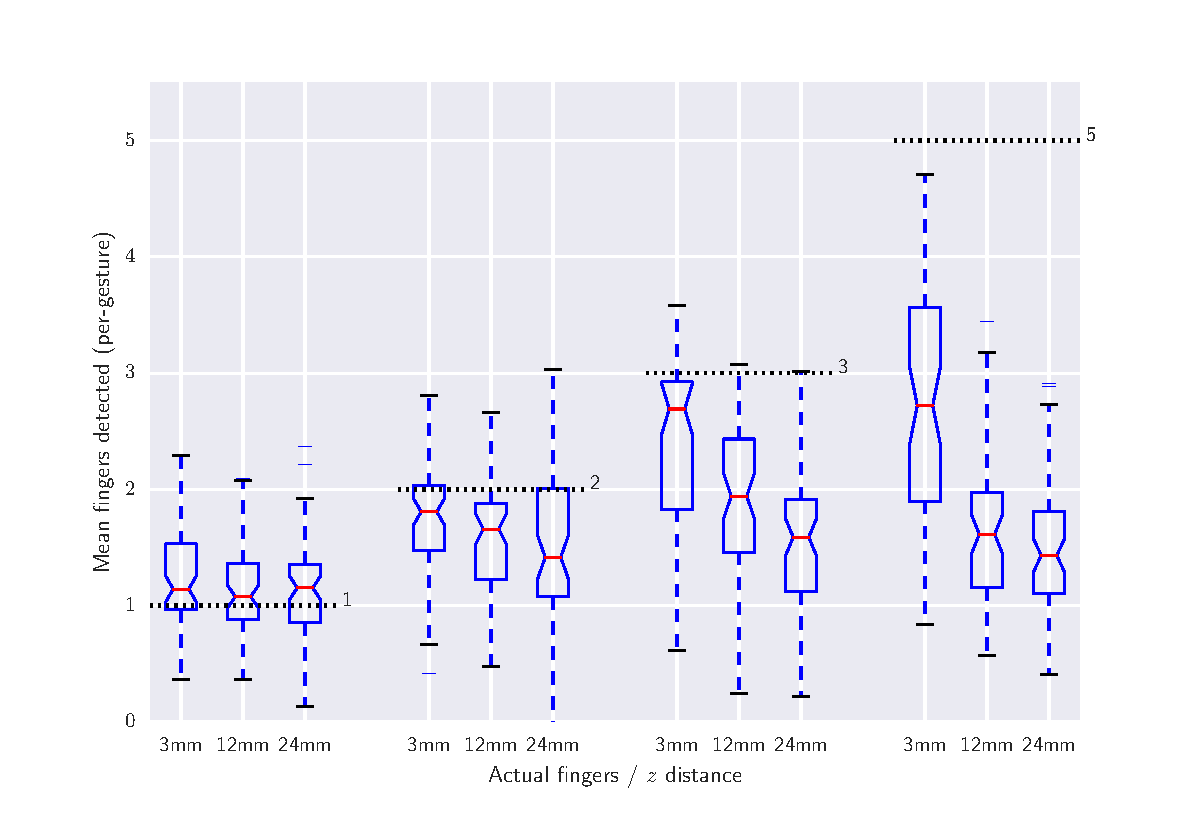
\includegraphics[width=1.0\linewidth]{images/boxplot_finger_distance.pdf}    

%     \caption{Average number of fingers detected by the touch sensor at different heights above the surface, averaged over all gestures. Dashed lines indicate
%     the true number of fingers present. The Box plots include bootstrapped uncertainty notches for the median. It is clear that the device is biased toward 
%     undercounting fingers, particularly at higher $z$ distances.
%     }

%     % use the notation fig:name to cross reference a figure
%     \label{fig:boxplot} 
% \end{figure}


%==================================================================================================================================
\chapter{Conclusion}

\section{Summary}

Cheyyan's development process has been a meticulous one, combining a variety of software engineering approaches and utilising state-of-the-art technology to provide a reliable and user-friendly time management tool. Cheyyan made sure that software development was approached in a balanced way by implementing agile approaches, version control systems like GitHub, and intentional testing practices. They placed a strong emphasis on quality assurance, cooperation, and flexibility in response to changing requirements.

Cheyyan's interface, backend, and integration with third-party tools are all designed with scalability, security, and user experience in mind. SQLite's selection as the backend framework offers a solid basis for handling intricate tasks, while Firebase Authentication improves user authentication and security. The dynamic and fluid front end made possible by the Flutter framework encourages accessibility and performance optimisation.

Additionally, Cheyyan's connection with third-party technologies such as PythonAnywhere for hosting scripts and fitness APIs like Google Fit and iOS Health App demonstrates a forward-thinking approach to enhancing user engagement and functionality. Cheyyan preserves moral values while offering beneficial incentives to users by addressing ethical issues including avoiding copyrighted content in prize prizes via the LibGen API in an ethical manner.

Insightful results were obtained from the assessment of Cheyyan's efficiency in improving time management abilities using gamification components. Overall, users like the task management aspects of the app and found it to be straightforward to utilise. To improve the user experience, there were recommendations made for increasing task customisation and quest clarity. Although the rewards programme was usually easy to understand, questions were brought up regarding the suitability of the prizes and sporadic problems with redemption. Participants indicated a desire to utilise Cheyyan in the long run, despite some reported technical difficulties, showing their perception of Cheyyan's worth in increasing productivity. These findings highlight the need for continued technological improvement, improved goal clarity, improved incentive systems, and the addition of more task management features to further strengthen Cheyyan's capacity to assist users in time management. This supports the objectives of gamification, as it emphasizes the importance of user engagement and motivation in achieving productivity goals, highlighting Cheyyan as a valuable tool for time management in today's competitive mobile application landscape.

To sum up, Cheyyan offers a complete solution for people who want to prioritise their health and well-being above time management abilities. Cheyyan provides a smooth and user-friendly experience by utilising the most recent developments in software engineering and technology integration, enabling users to successfully meet their productivity objectives.

\section{Future Work}
The development of Cheyyan has laid a solid foundation for its role as a reliable and user-friendly time management tool. However, there are several areas where future work could further enhance its functionality and user experience.

\subsection{Enhanced Task Customization}
One area for improvement is the customization of tasks within Cheyyan. By allowing users to personalize task attributes such as priority levels, deadlines, and reminders, the app can better align with individual preferences and workflow management styles. Implementing advanced task management features could significantly enhance user satisfaction and productivity.

\subsection{Improved Quest Clarity}
Feedback from users highlighted the importance of clear instructions and objectives in quest completion. Future iterations of Cheyyan could focus on refining quest structures and providing more detailed guidance to users. Enhancing quest clarity will facilitate smoother user interactions and increase engagement with gamified elements.

\subsection{Optimized Reward System}
While the reward system in Cheyyan was generally well-received, there were concerns raised about the suitability of rewards and occasional issues with redemption. Future work could involve refining the reward mechanism to offer more relevant and enticing incentives for users. Additionally, streamlining the redemption process will contribute to a more seamless user experience.

\subsection{Technical Stability and Performance Optimization}
Addressing reported technical issues, such as latency, crashes, and bugs, is essential for maintaining user satisfaction and app reliability. Continued efforts in technical stability and performance optimization will ensure a smooth and uninterrupted user experience. Regular updates and bug fixes will contribute to the long-term success of Cheyyan.

\subsection{Integration of Additional Features}
Expanding Cheyyan's feature set to include functionalities such as goal tracking, habit formation, and collaborative task management could further enhance its utility for users. Integration with emerging technologies and platforms, as well as partnerships with relevant service providers, can enrich Cheyyan's capabilities and provide users with a comprehensive time management solution.

\subsection{Ethical Considerations and Content Moderation}
Given the ethical considerations surrounding content access and usage, Cheyyan must continue to prioritize ethical content sourcing and moderation practices. Ensuring compliance with copyright regulations and promoting responsible content sharing will uphold Cheyyan's moral values and foster trust among users.

In conclusion, ongoing development efforts should focus on refining existing features, addressing user feedback, and incorporating innovative functionalities to elevate Cheyyan as a leading solution for time management and productivity enhancement. By staying responsive to user needs and technological advancements, Cheyyan can continue to evolve as a valuable tool for individuals striving to achieve their goals while prioritizing health and well-being.

% Summarise the whole project for a lazy reader who didn't read the rest (e.g. a prize-awarding committee).
% \section{Guidance}
% \begin{itemize}
%     \item
%         Summarise briefly and fairly.
%     \item
%         You should be addressing the general problem you introduced in the
%         Introduction.        
%     \item
%         Include summary of concrete results (``the new compiler ran 2x
%         faster'')
%     \item
%         Indicate what future work could be done, but remember: \textbf{you
%         won't get credit for things you haven't done}.
% \end{itemize}

%==================================================================================================================================
%
% 
%==================================================================================================================================
%  APPENDICES  

\begin{appendices}

\chapter{Appendices}

\begin{figure}[h]
    \centering
    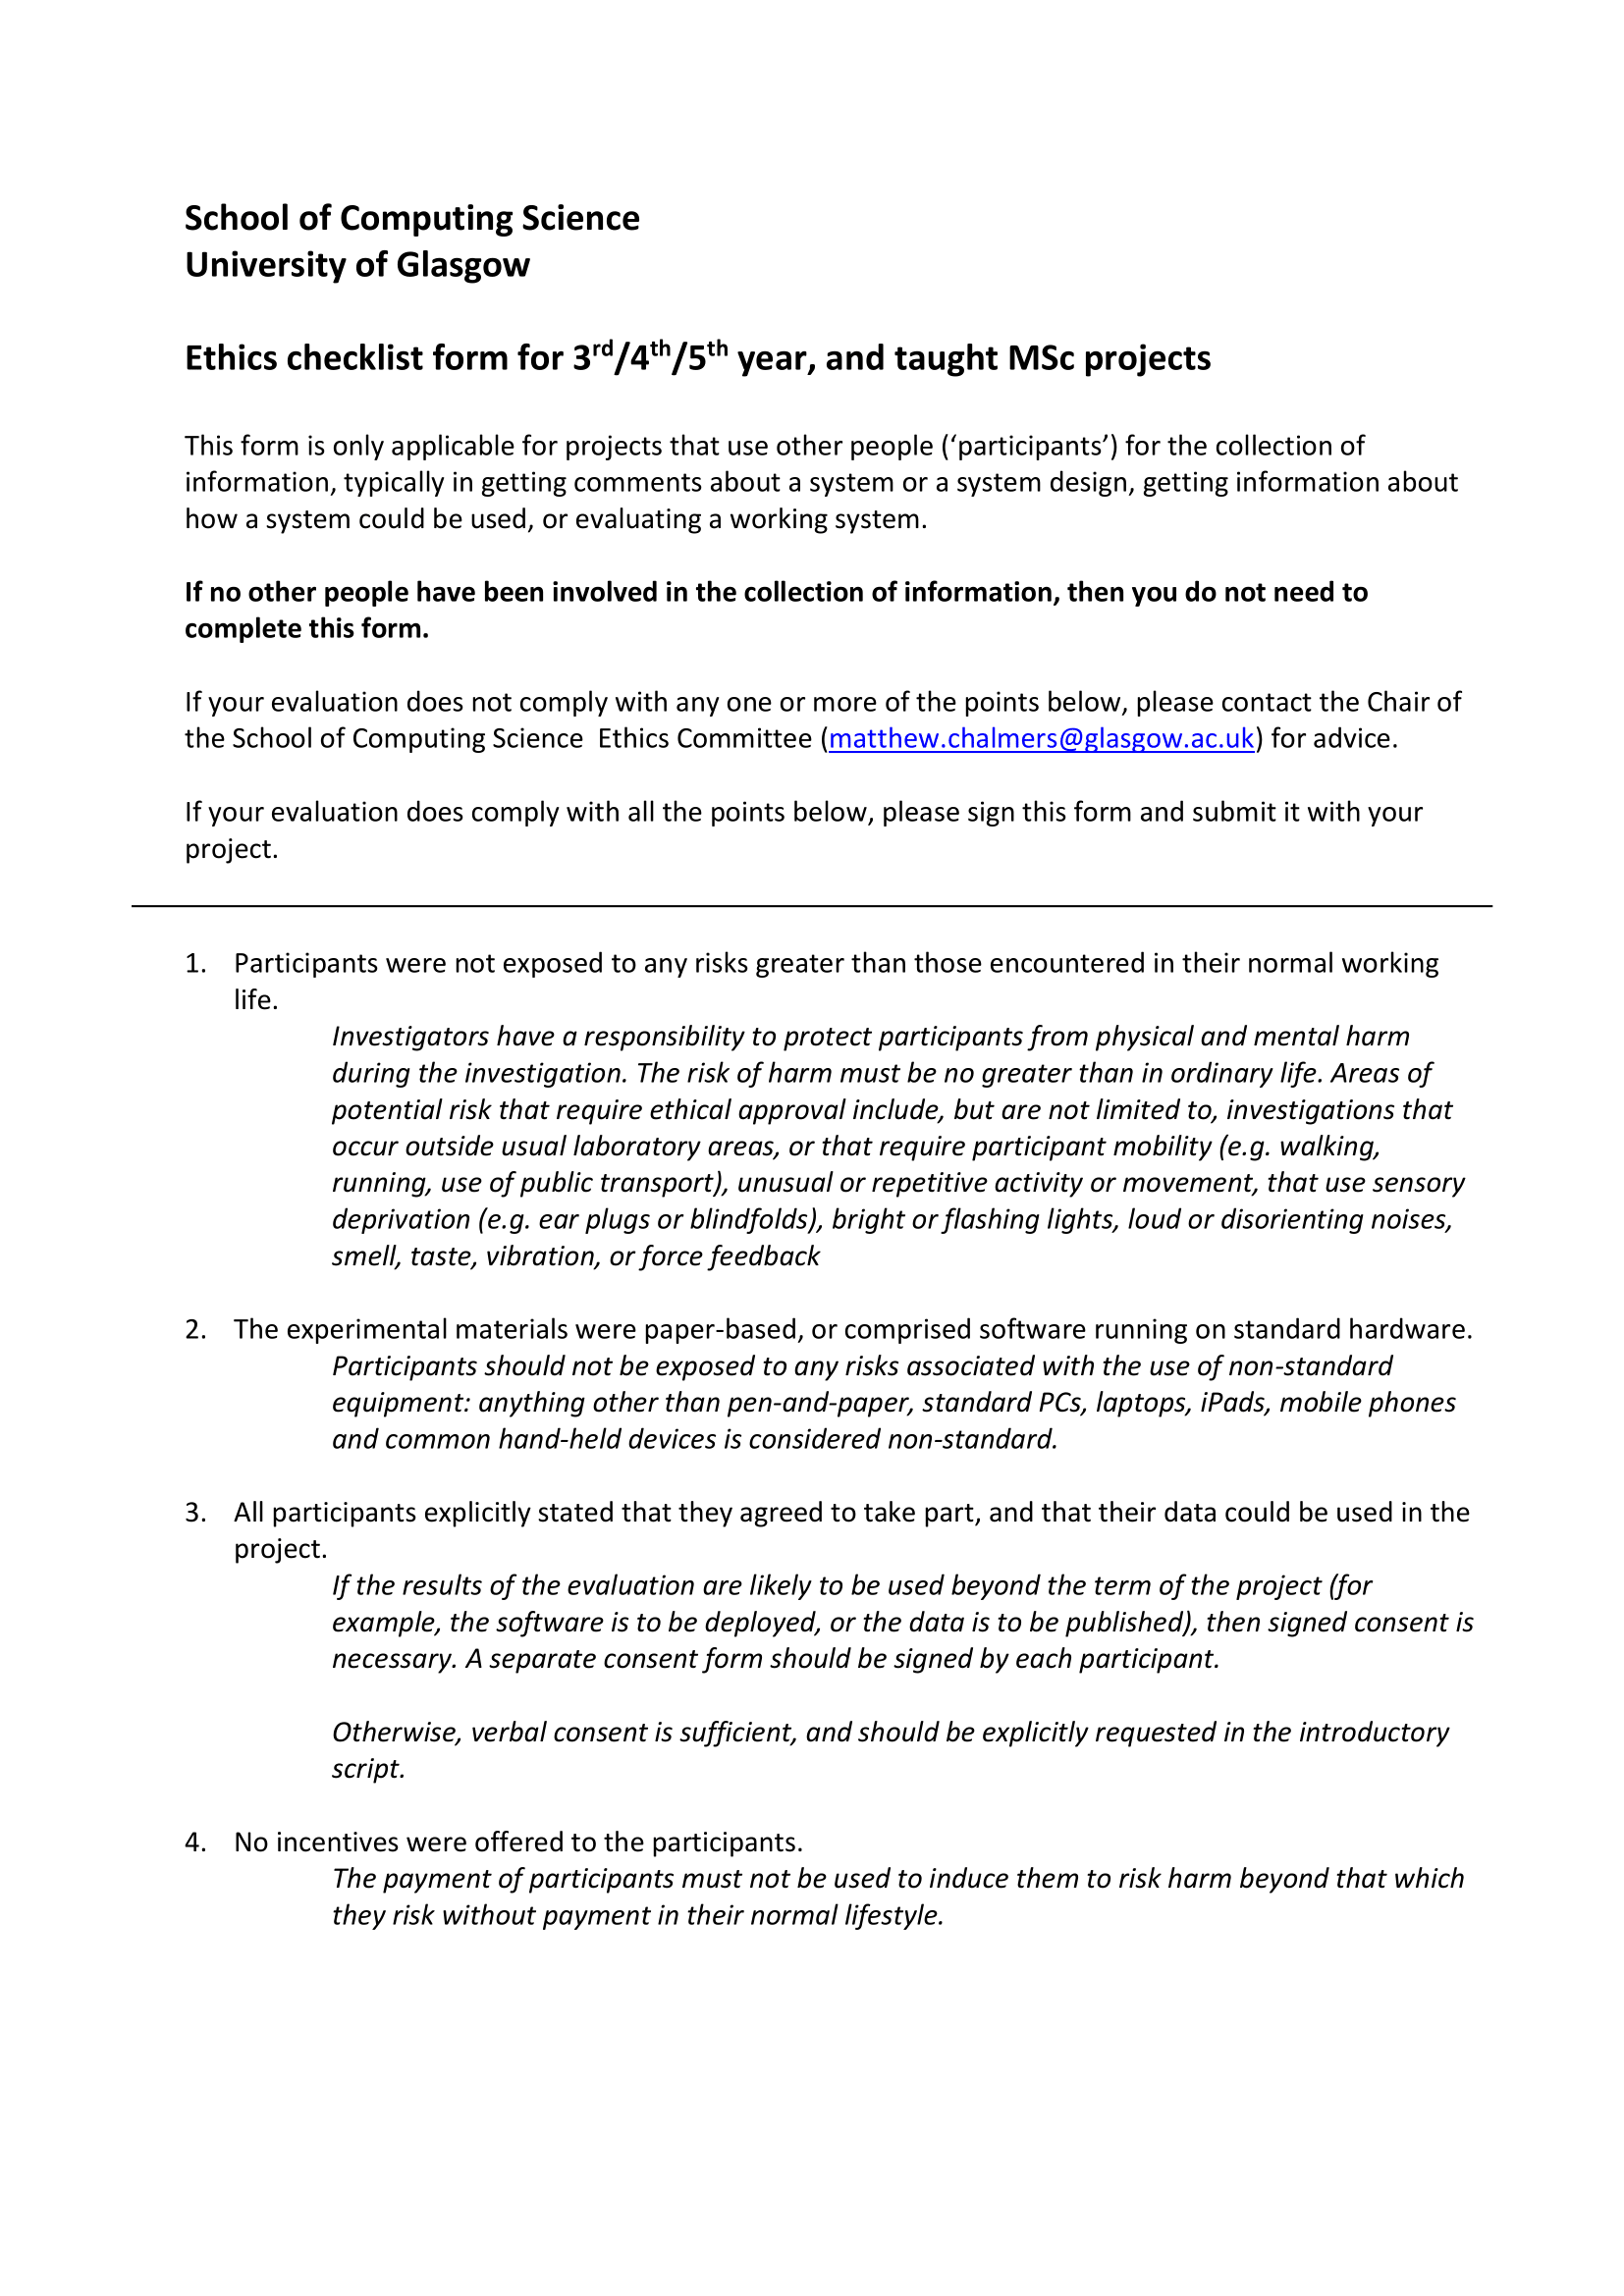
\includegraphics[height=20cm]{images/Media_515048_smxx-1.png}
\end{figure}

\begin{figure}[h]
    \centering
    
\includegraphics[height=20cm]{images/34a2091fe24cc99d9a76a9e1640fc37a-1[1].png}
    \caption{Ethics Checklist}

\end{figure}

\begin{figure}[h]
    \centering
    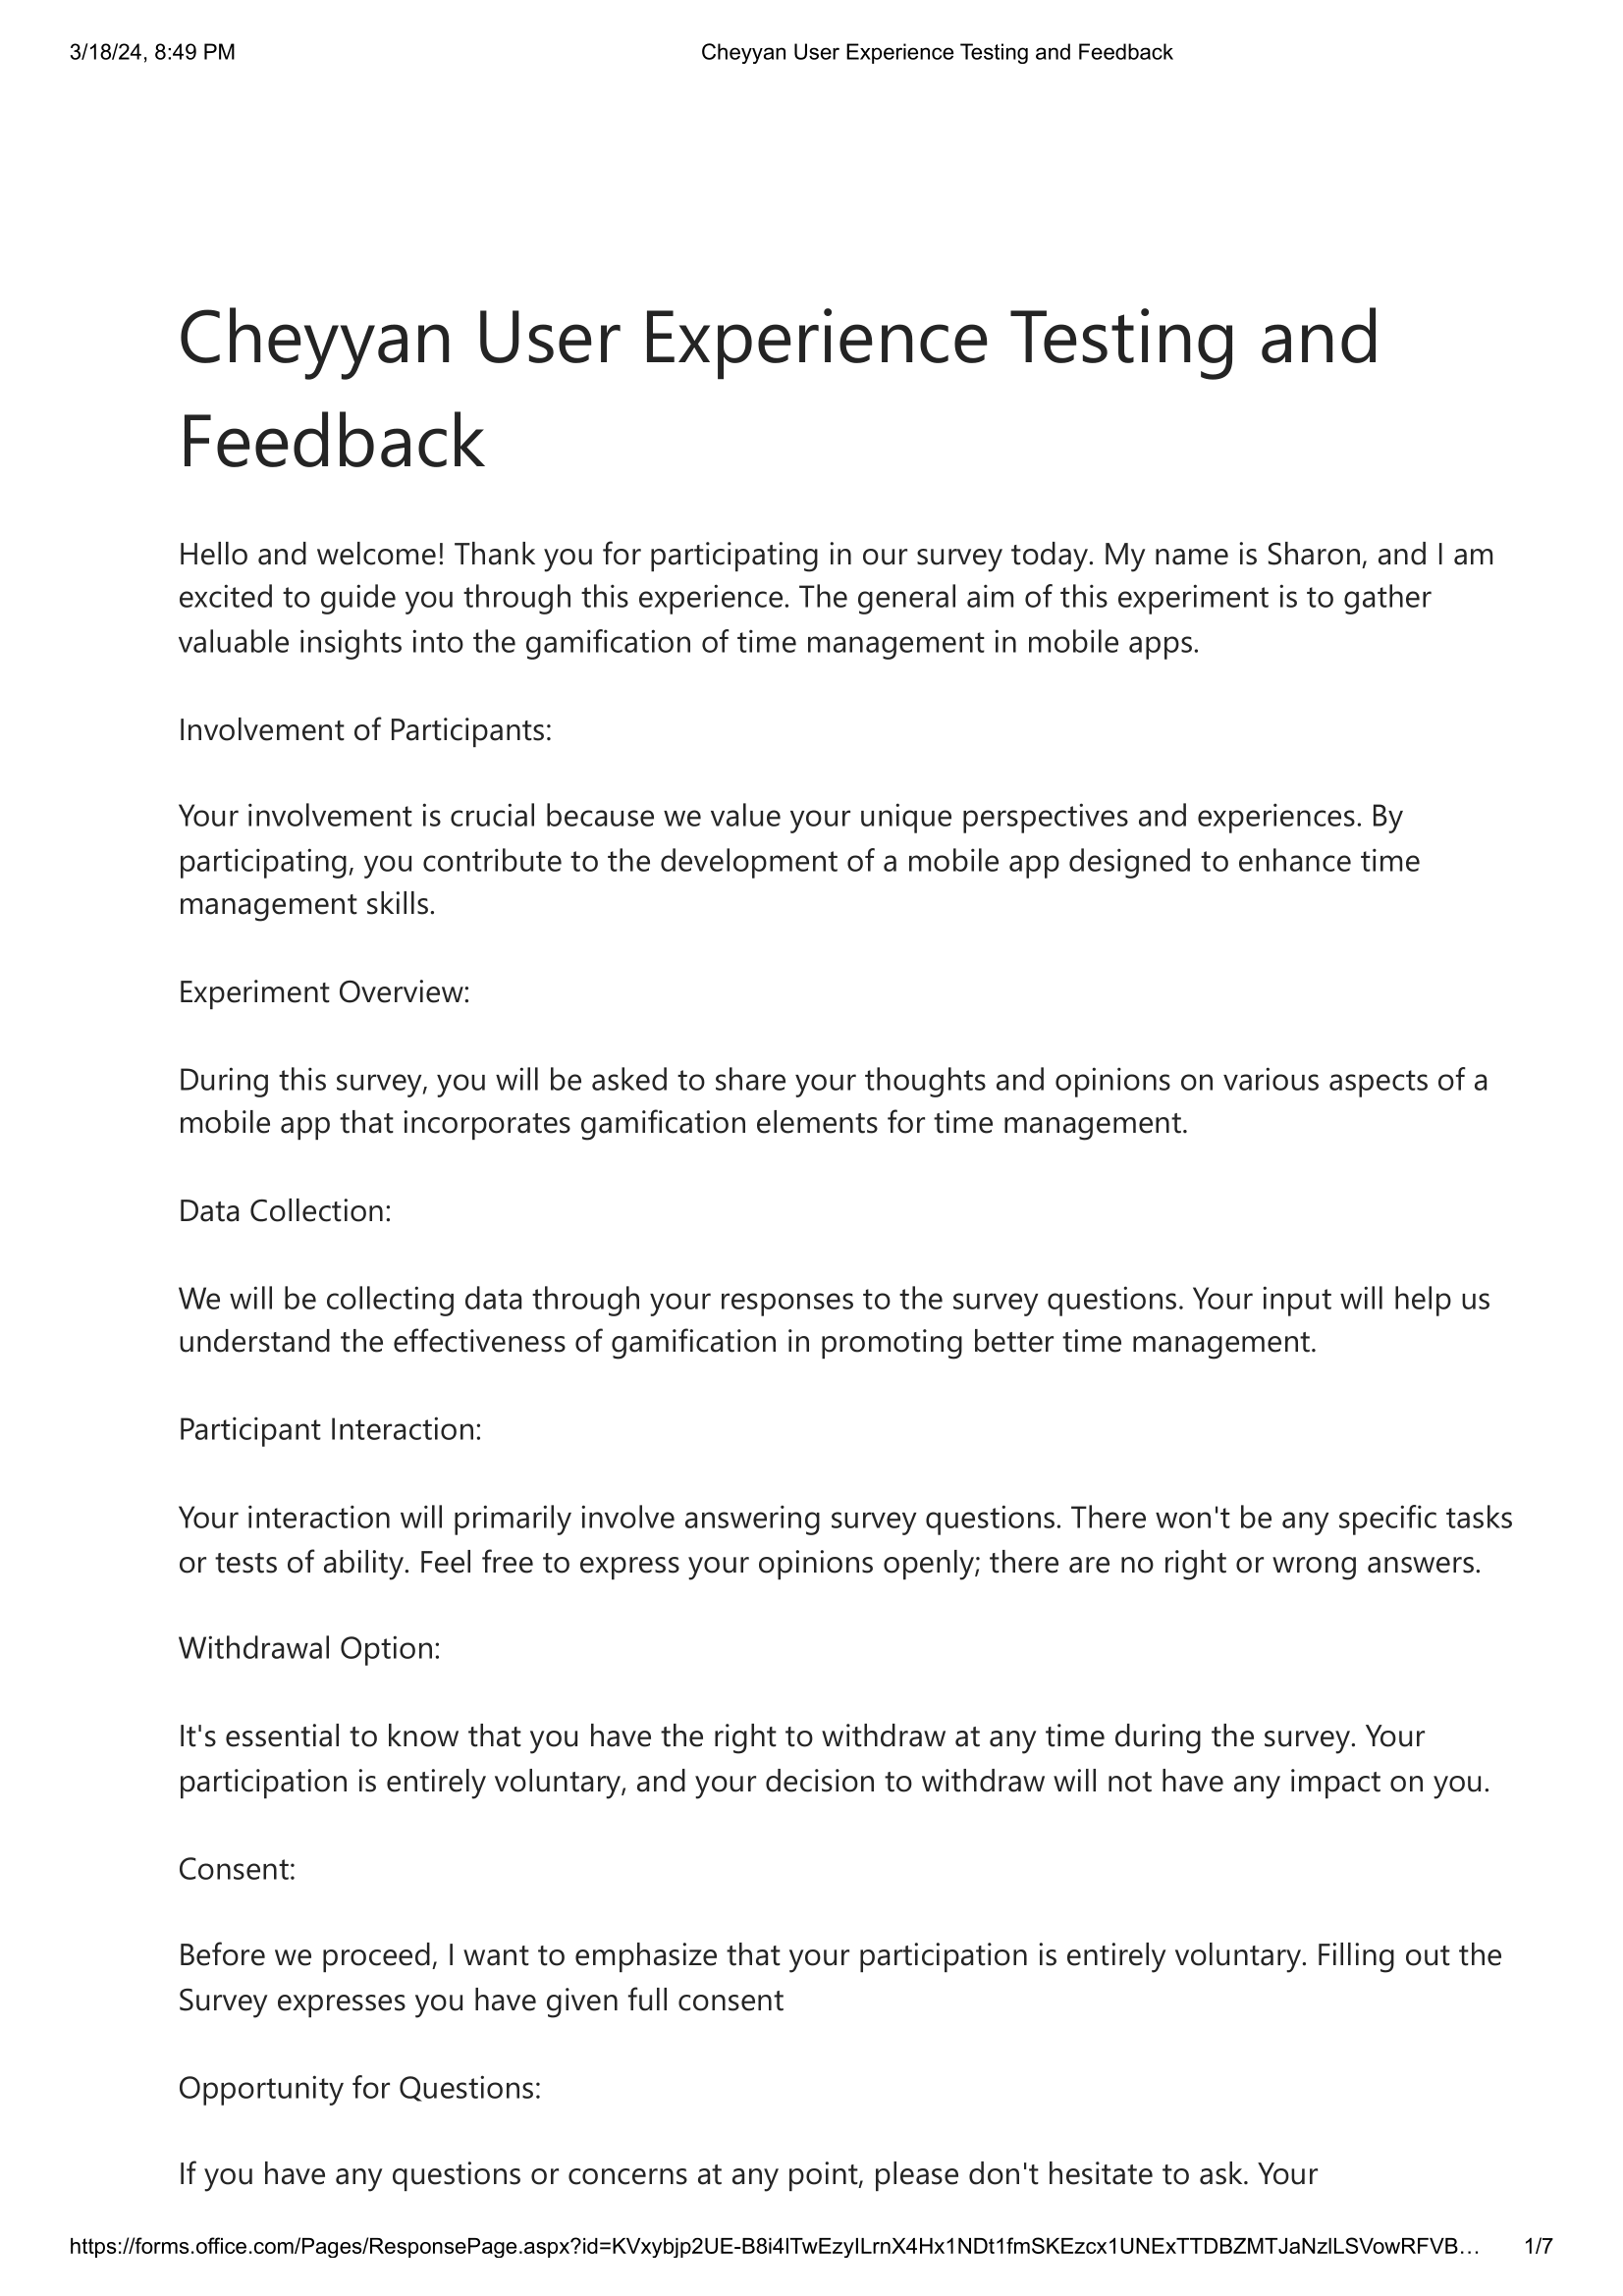
\includegraphics[height=20cm]{images/Cheyyan User Experience Testing and Feedback-1.png}
\end{figure}

\begin{figure}[h]
    \centering
    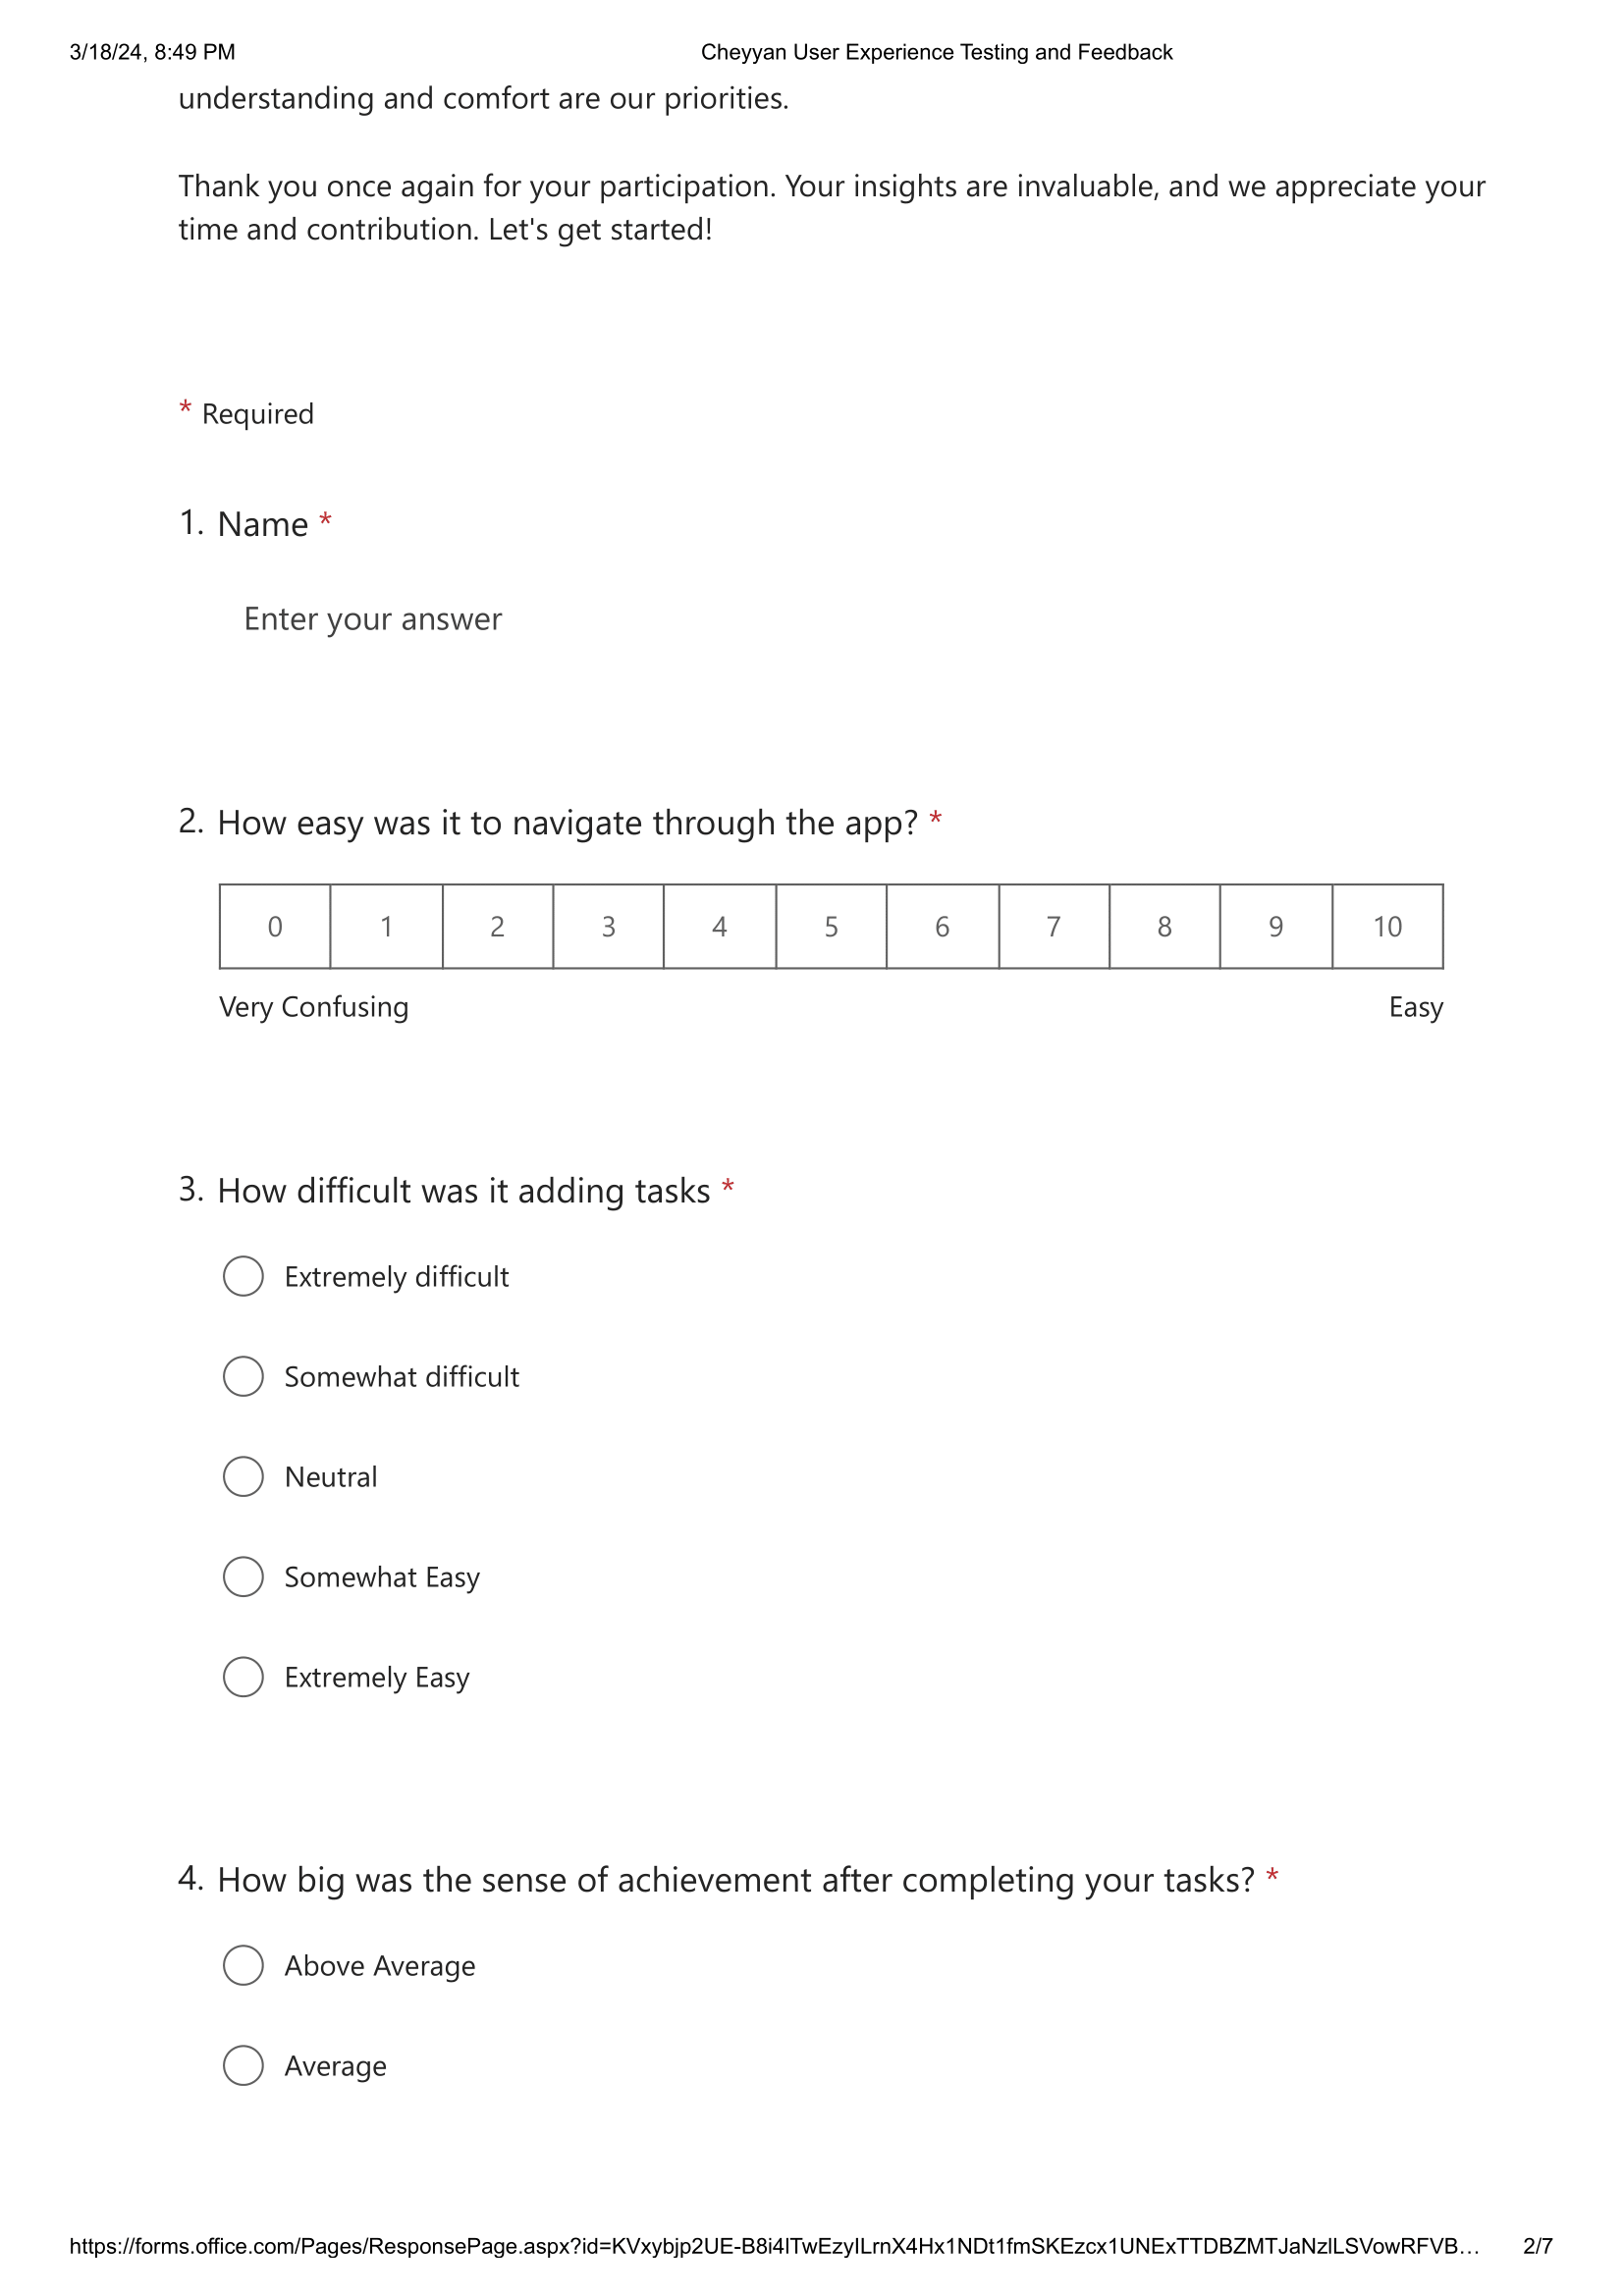
\includegraphics[height=20cm]{images/Cheyyan User Experience Testing and Feedback-2.png}
\end{figure}

\begin{figure}[h]
    \centering
    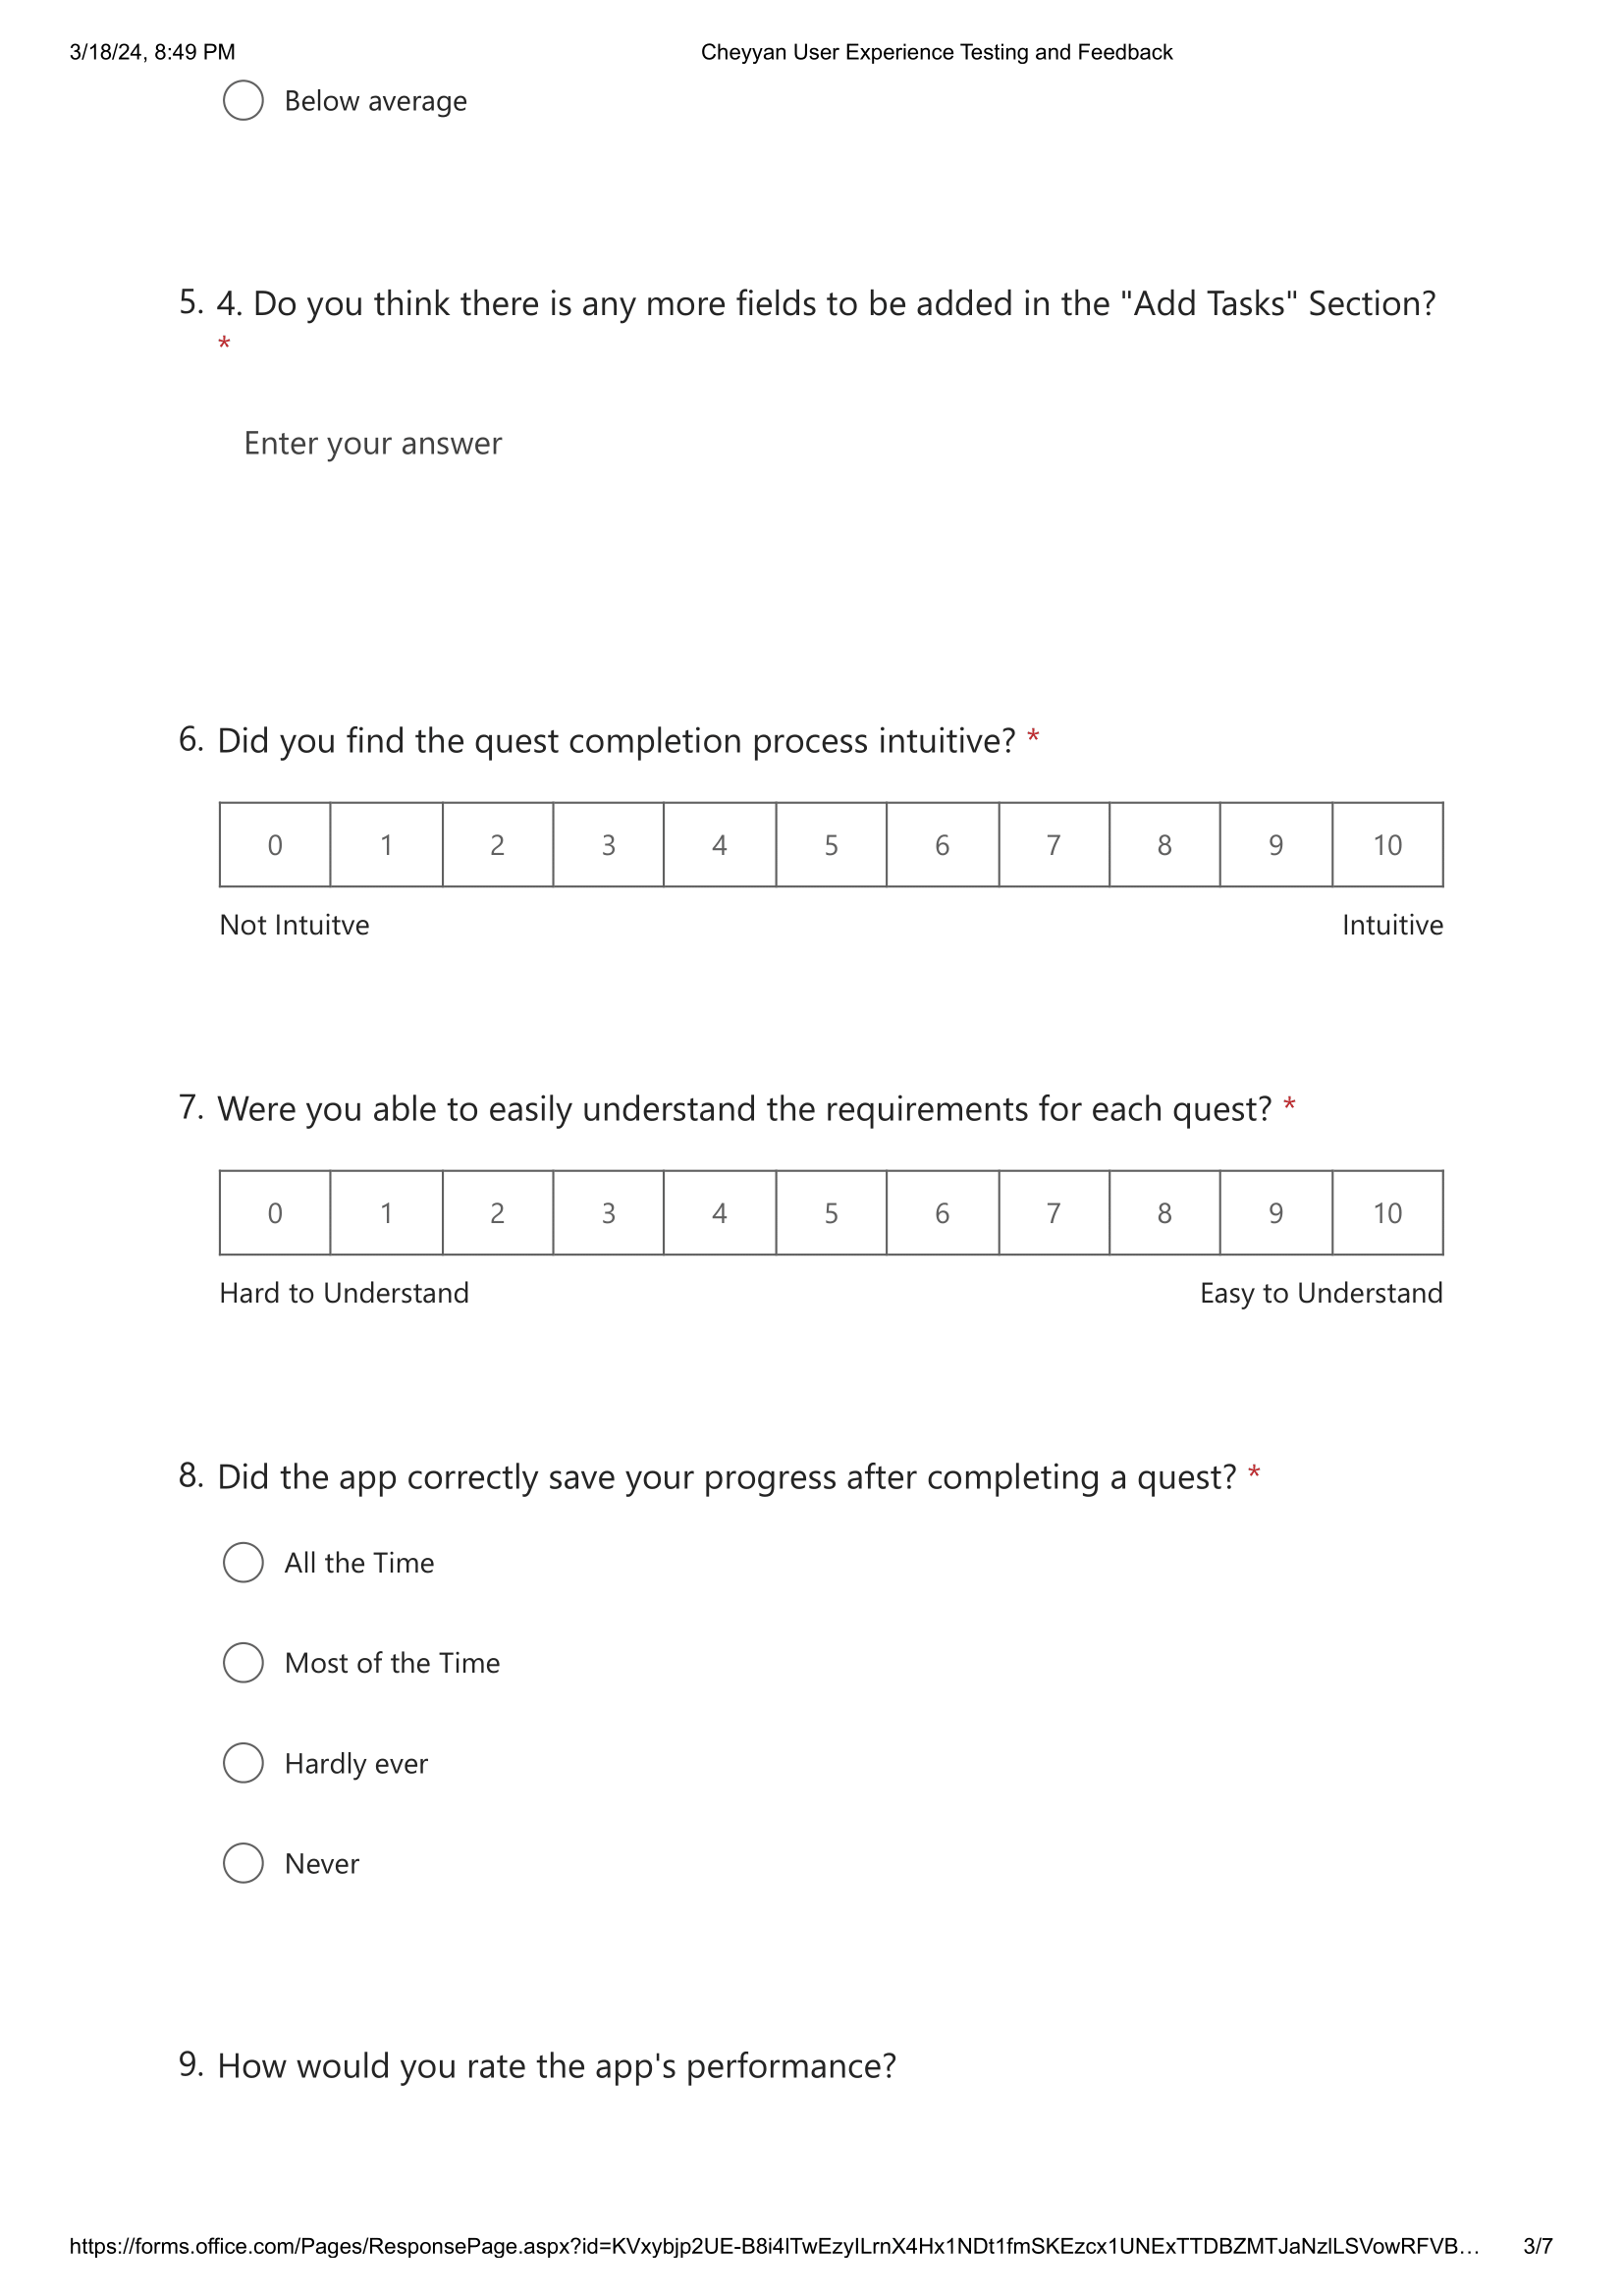
\includegraphics[height=20cm]{images/Cheyyan User Experience Testing and Feedback-3.png}
\end{figure}

\begin{figure}[h]
    \centering
    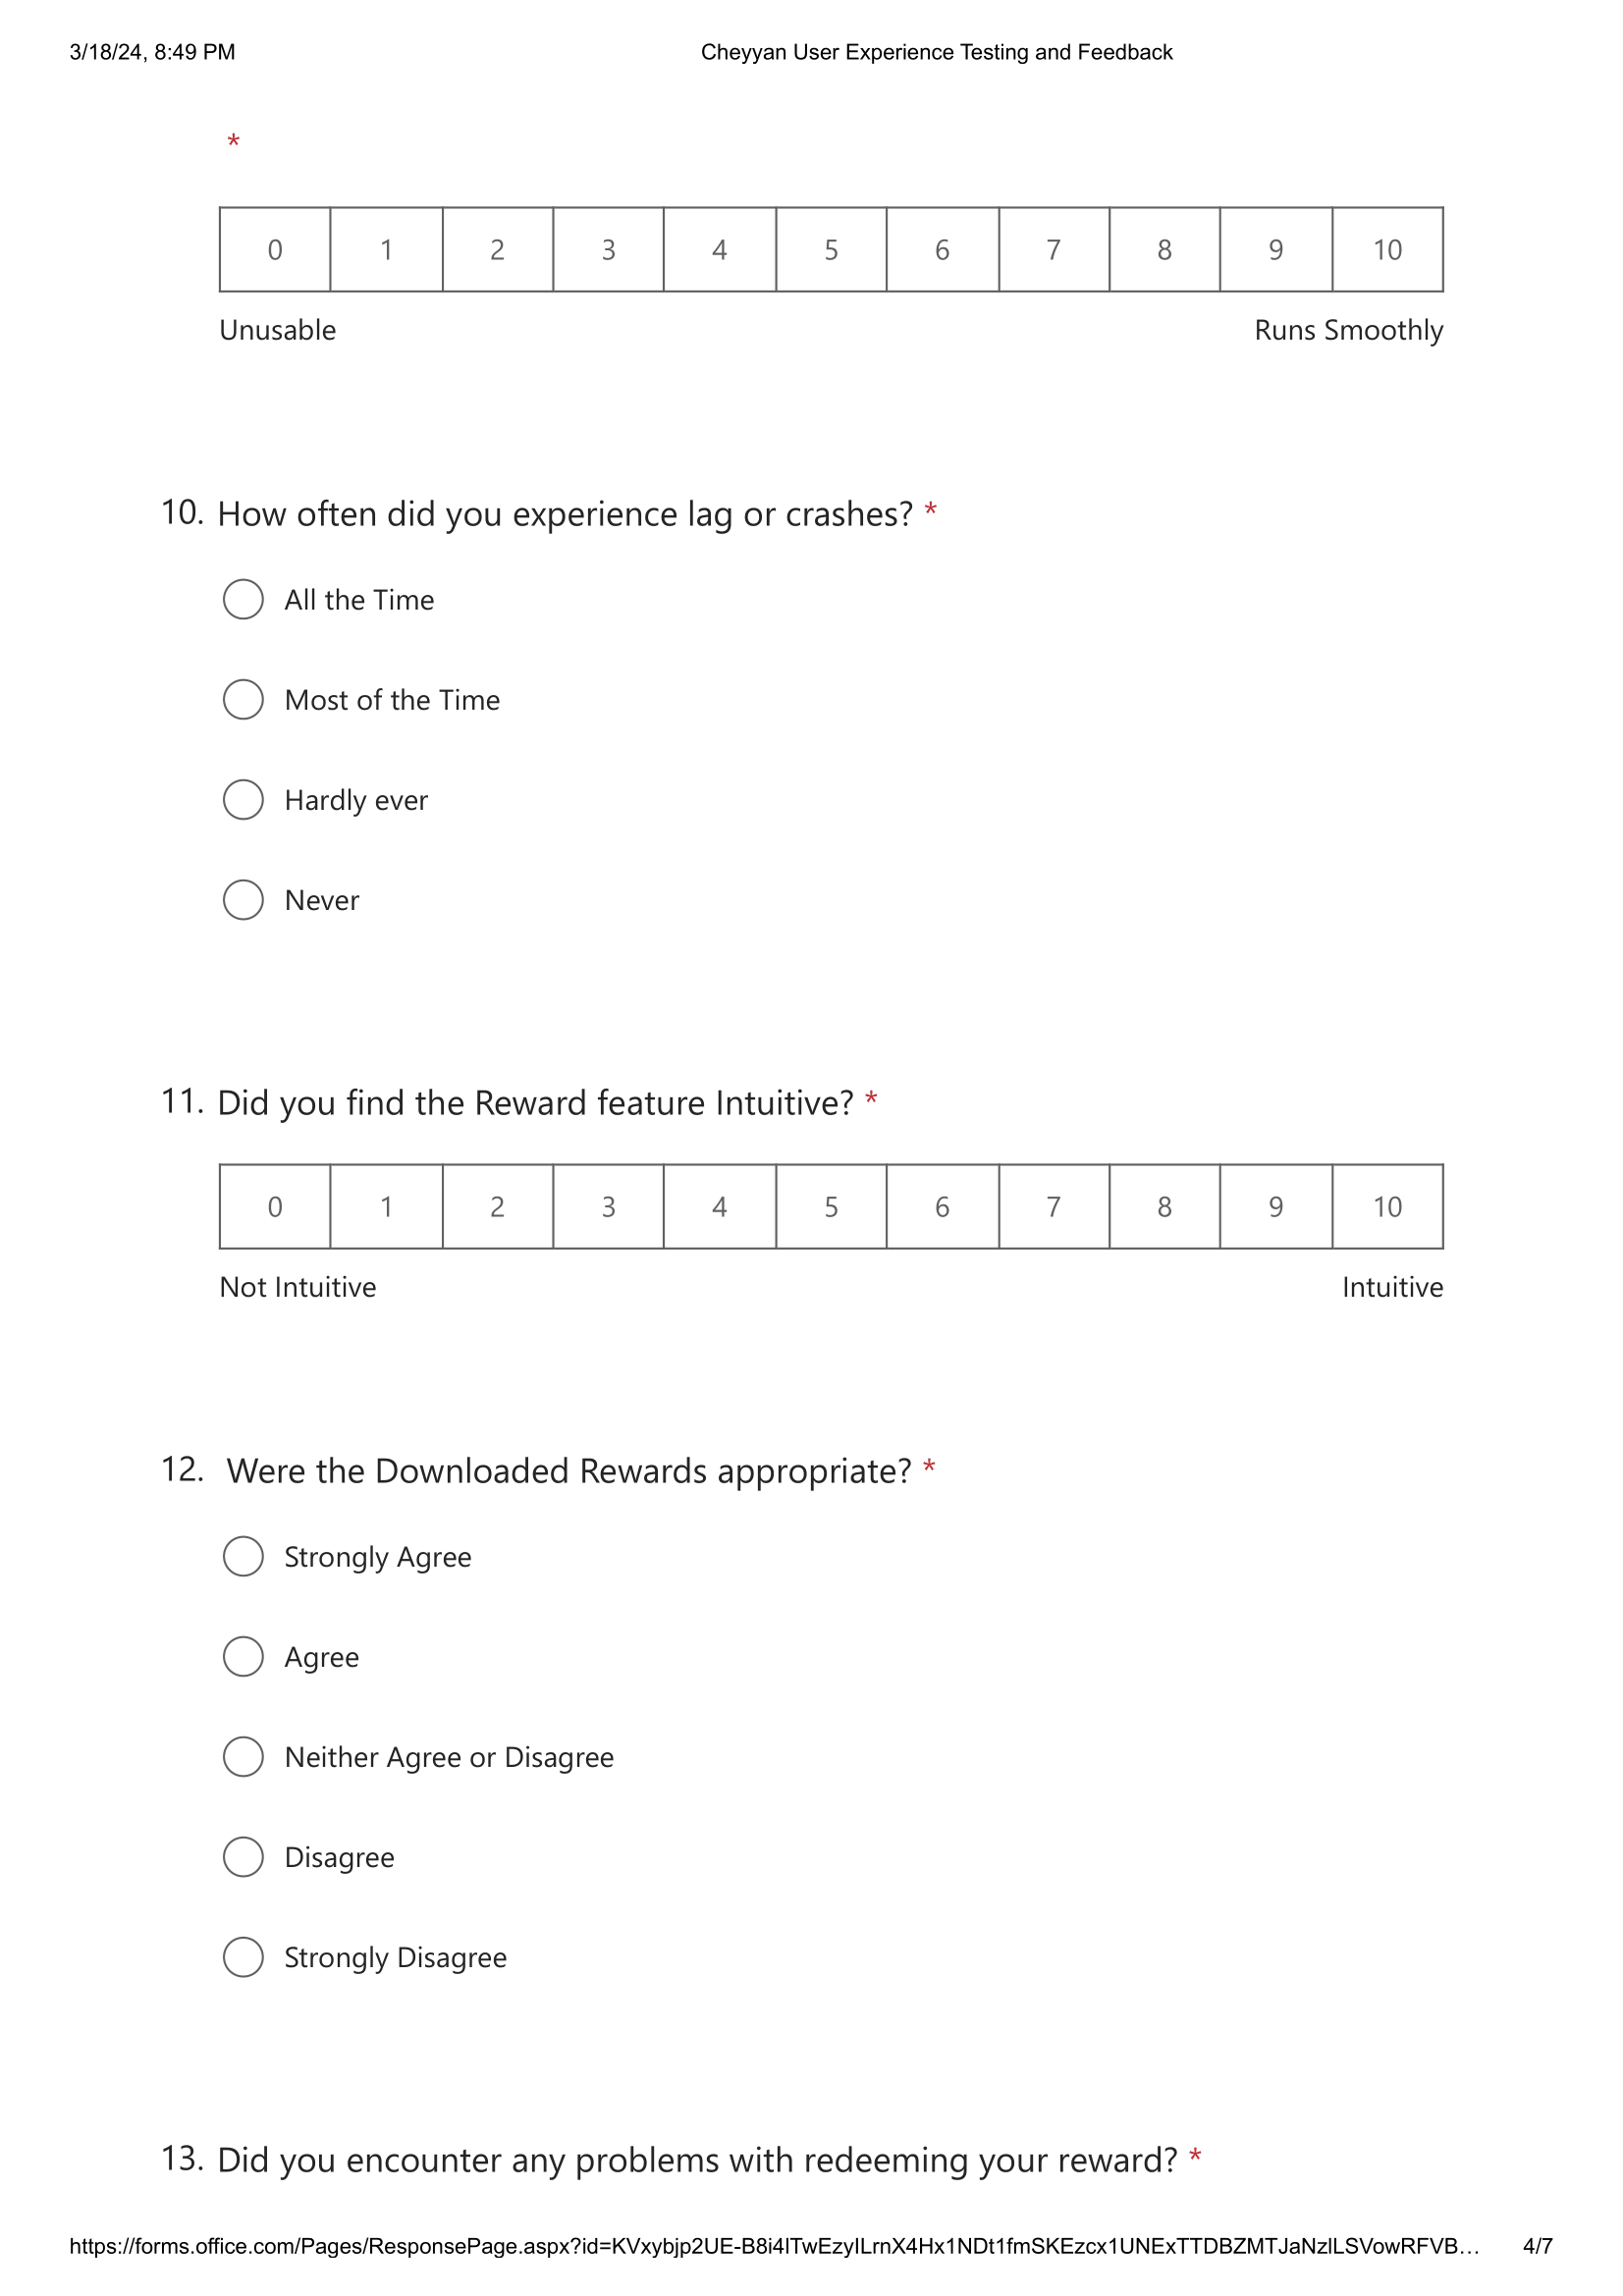
\includegraphics[height=20cm]{images/Cheyyan User Experience Testing and Feedback-4.png}
\end{figure}

\begin{figure}[h]
    \centering
    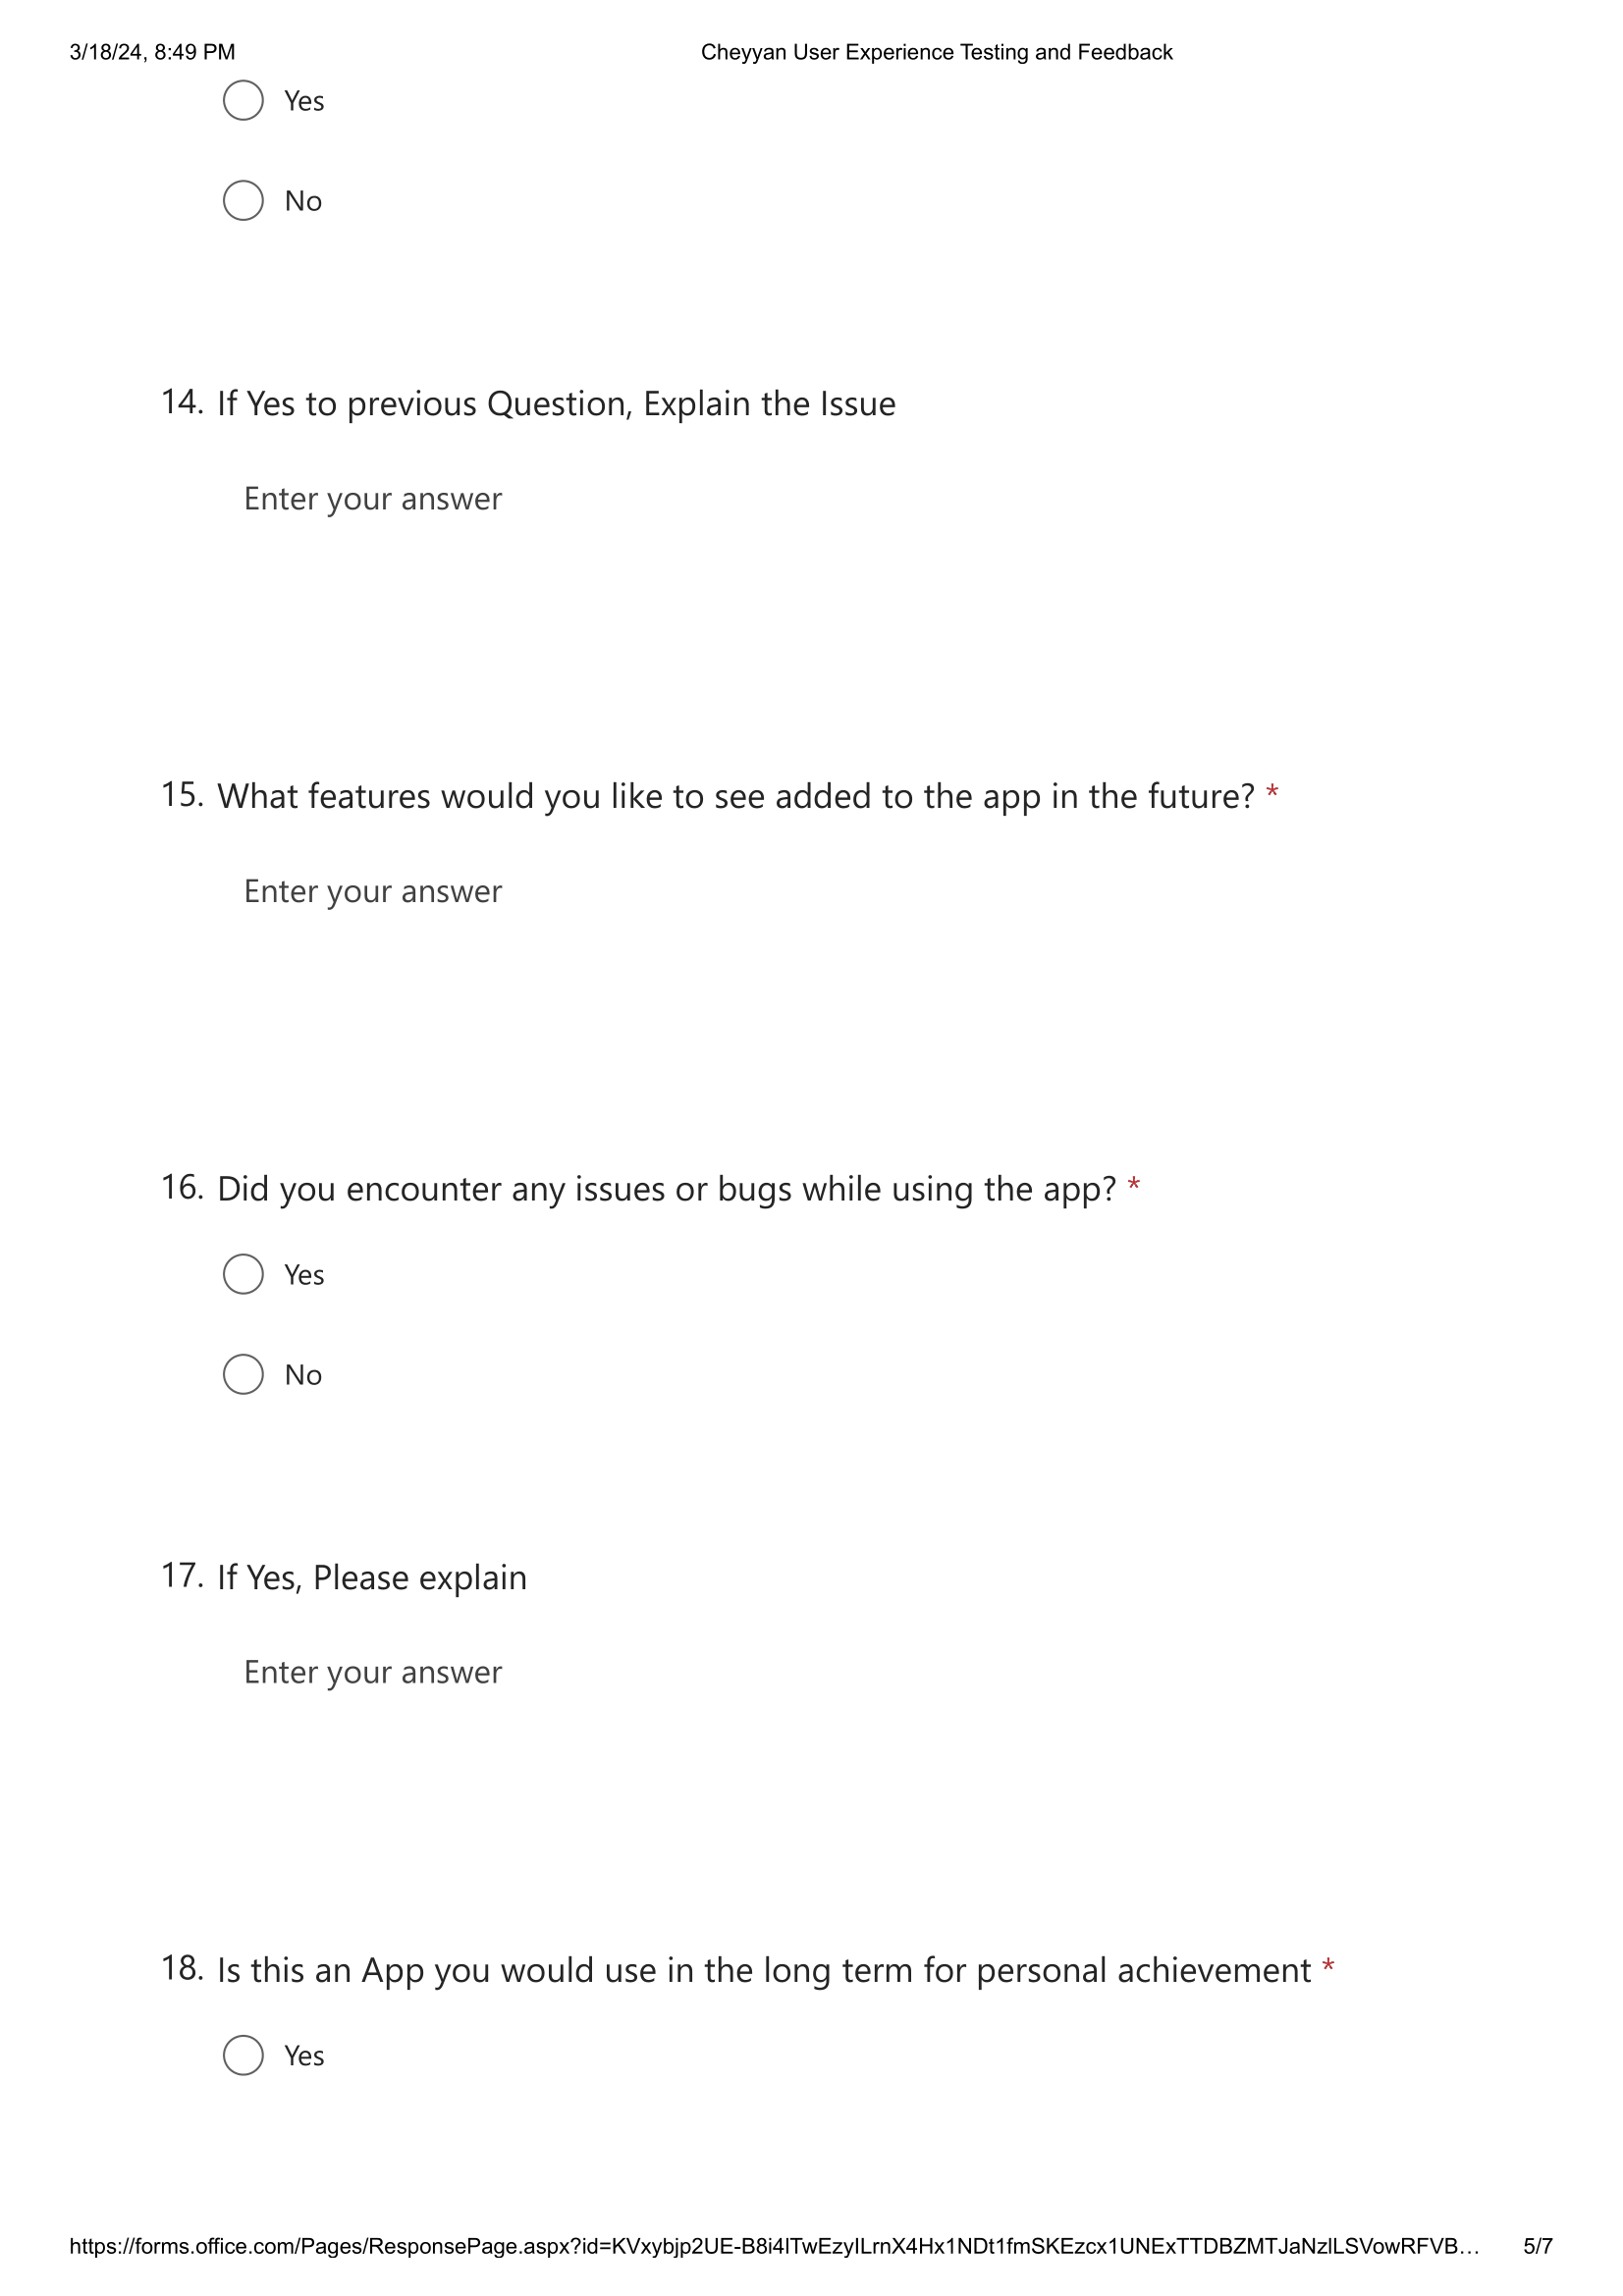
\includegraphics[height=20cm]{images/Cheyyan User Experience Testing and Feedback-5.png}
\end{figure}

\begin{figure}[h]
    \centering
    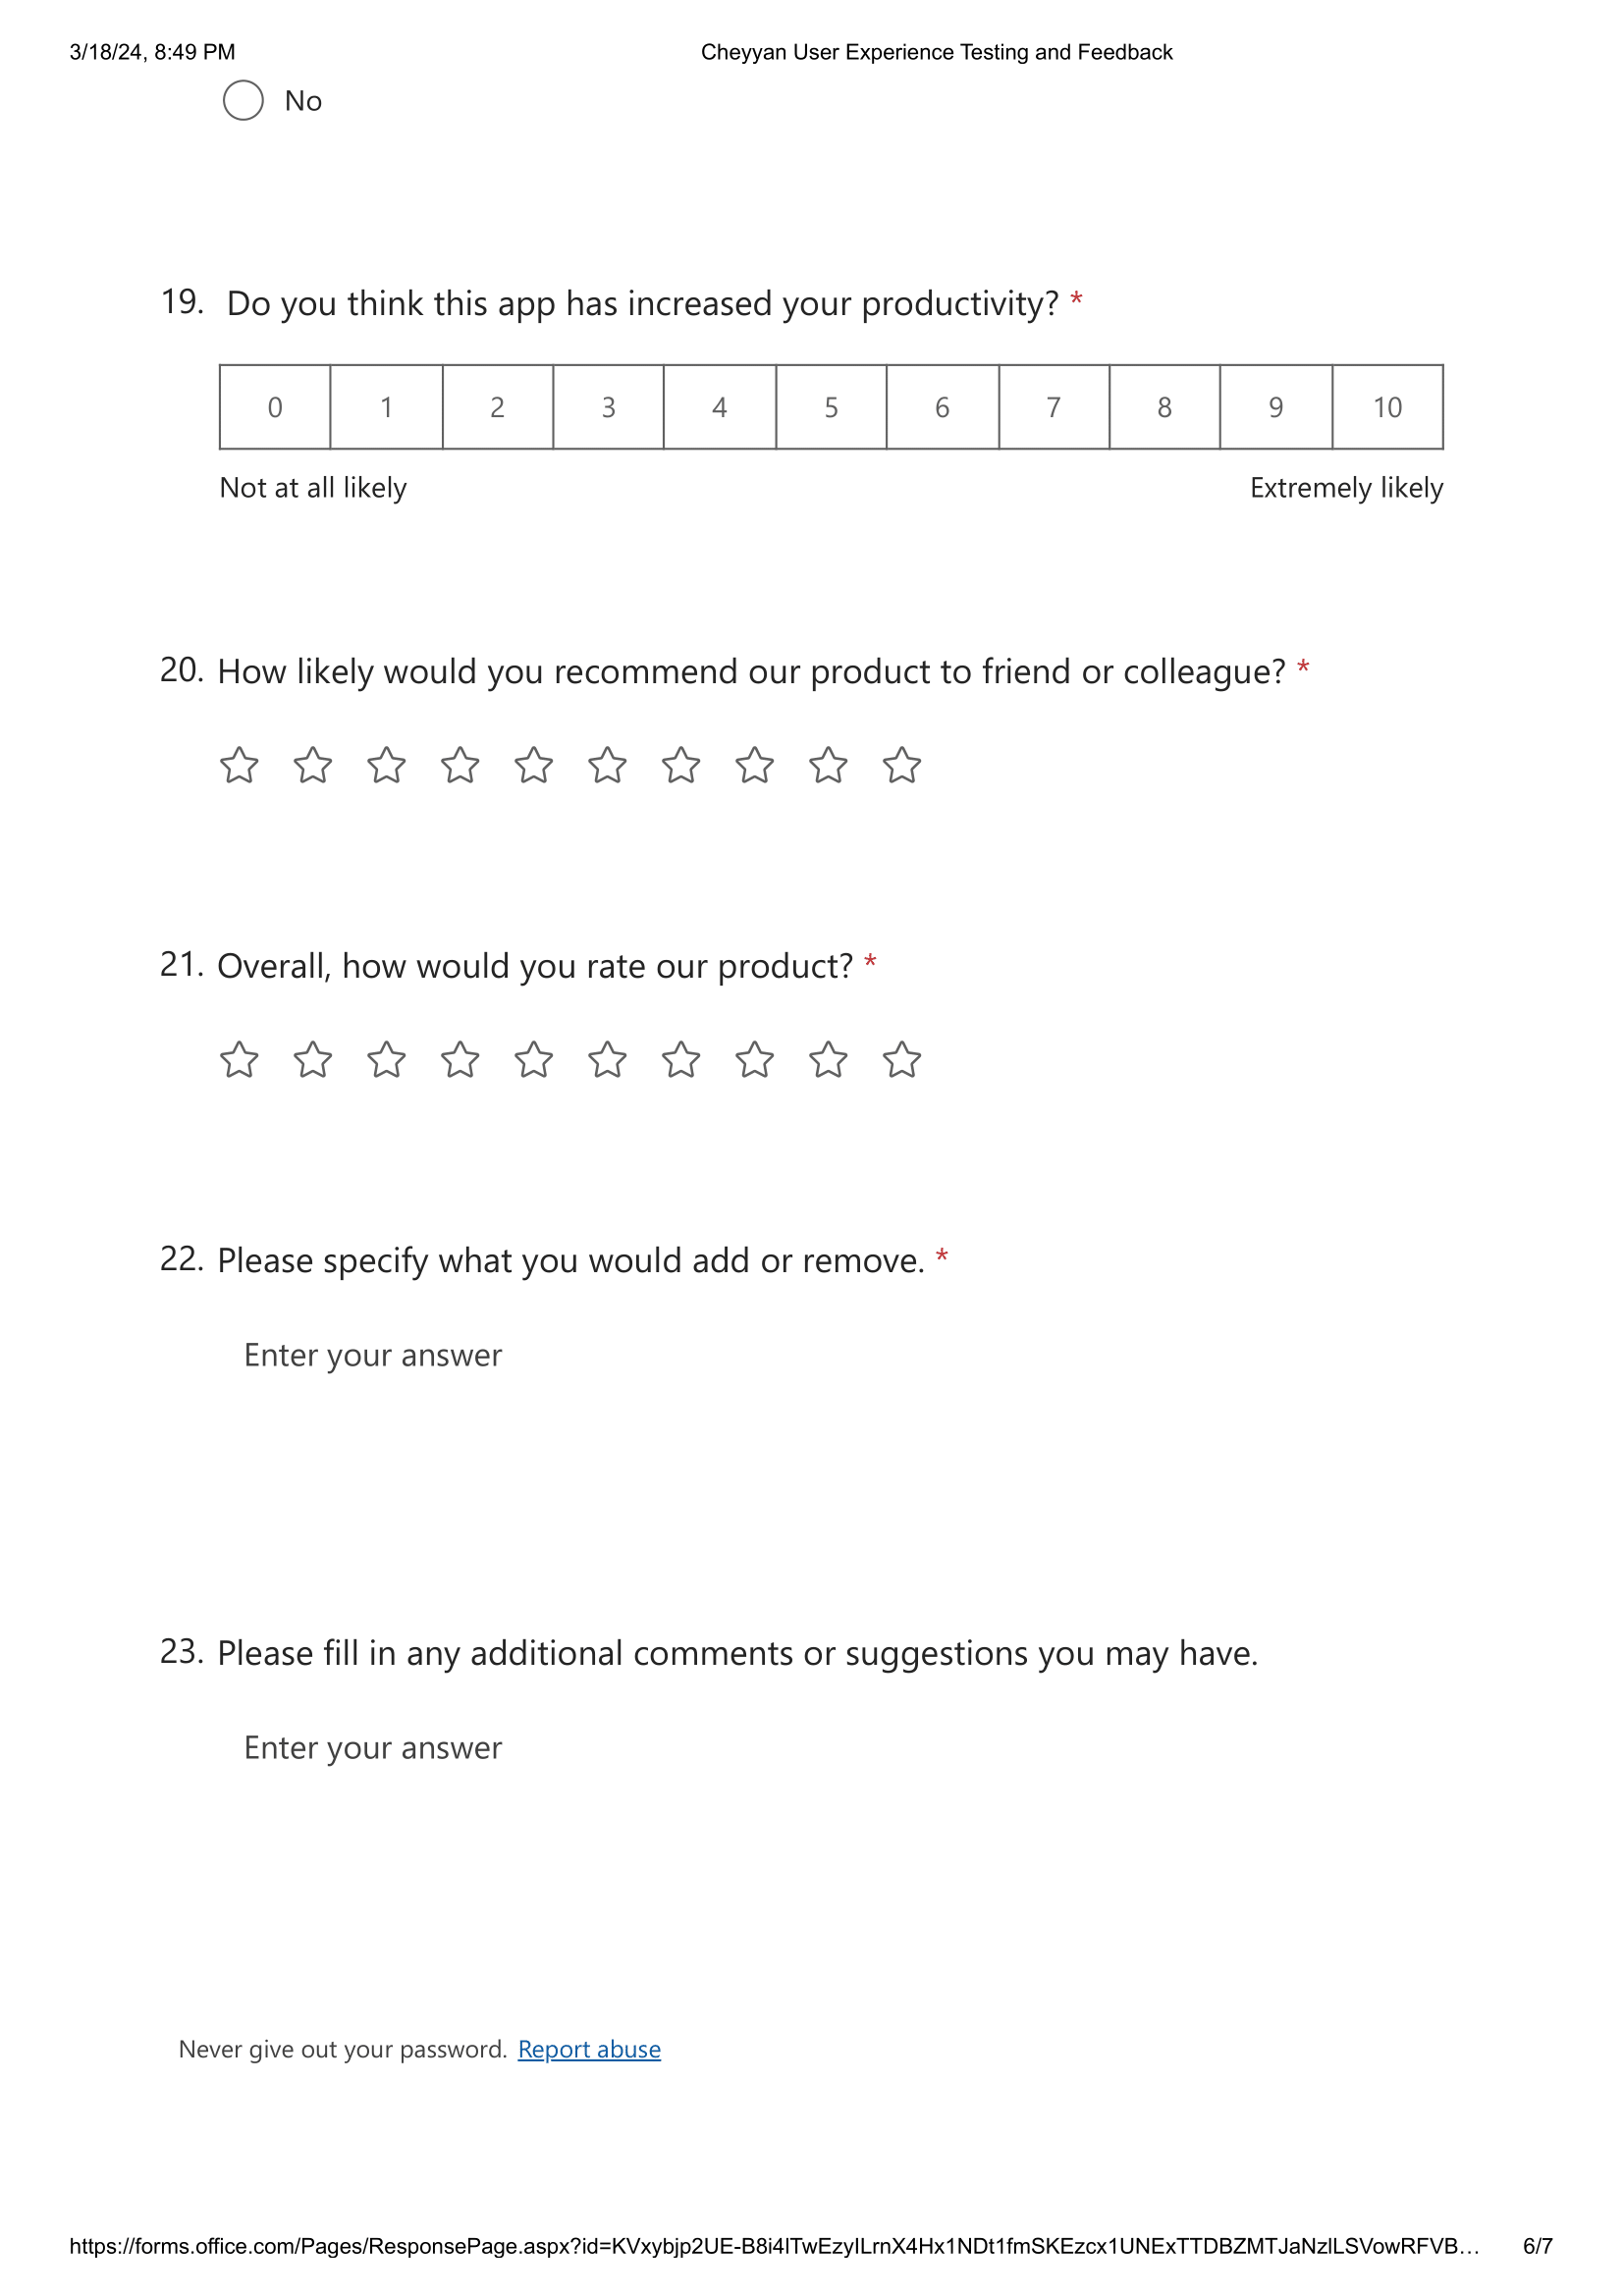
\includegraphics[height=20cm]{images/Cheyyan User Experience Testing and Feedback-6.png}
\end{figure}




% Typical inclusions in the appendices are:

% \begin{itemize}
% \item
%   Copies of ethics approvals (required if obtained)
% \item
%   Copies of questionnaires etc. used to gather data from subjects.
% \item
%   Extensive tables or figures that are too bulky to fit in the main body of
%   the report, particularly ones that are repetitive and summarised in the body.

% \item Outline of the source code (e.g. directory structure), or other architecture documentation like class diagrams.

% \item User manuals, and any guides to starting/running the software.

% \end{itemize}

% \textbf{Don't include your source code in the appendices}. It will be
% submitted separately.

\end{appendices}

%==================================================================================================================================
%   BIBLIOGRAPHY   

% The bibliography style is abbrvnat
% The bibliography always appears last, after the appendices.

\bibliographystyle{abbrvnat}

\bibliography{l4proj}

\end{document}
